\documentclass[12pt, letter paper]{report}
\usepackage{amsmath}
\usepackage{amssymb}
\usepackage[spanish,activeacute]{babel}
\usepackage{csquotes}
\usepackage{diagbox}
\usepackage{float}
\usepackage[letterpaper, margin = 2cm]{geometry}
\usepackage{graphicx}
\usepackage{icomma}
\usepackage[utf8]{inputenc}
\usepackage{listings}
\usepackage{multirow}
\usepackage{pdflscape}
\usepackage{siunitx}
\usepackage{threeparttable}
\usepackage{tikz}
\usepackage{upquote} % Esto hace que las comillas sean rectas
\usepackage{CJKutf8}

\setlength{\intextsep}{12pt plus 2pt minus 2pt}

\sisetup{
  output-decimal-marker = {,}, % Coma para decimales
  exponent-product = \times,    % 'x' para notación científica
  separate-uncertainty = false, % Por si usas errores (2,5 +/- 0,1)
  per-mode = symbol            % Para usar km/h en lugar de km h^{-1}
}

\usetikzlibrary{er}
\tikzset{multi attribute/.style={attribute,double distance=1.5pt}}
\tikzset{derived attribute/.style={attribute,dashed}}
\tikzset{total/.style={double distance=1.5pt}}
\tikzset{every entity/.style={draw=orange,fill=orange!20}}
\tikzset{every attribute/.style={draw=red,fill=red!20}}
\tikzset{every relationship/.style={draw=blue,fill=blue!20}}

\makeatletter
\def\@makechapterhead#1{%
  \vspace*{50\p@}% Espacio inicial arriba
  {\parindent \z@ \raggedright \normalfont
    \ifnum \c@secnumdepth >\m@ne
      % Aquí unimos "Capítulo" + "Número" + "Título" en una sola línea
      \huge\bfseries \@chapapp\ \thechapter. \ #1\par
    \fi
    \interlinepenalty\@M
    \vskip 40\p@ % Espacio después del título
  }}
\makeatother

\newcommand{\key}[1]{\underline{#1}}
\renewcommand{\thechapter}{\Roman{chapter}}
\renewcommand{\thesection}{\arabic{chapter}.\arabic{section}}
\renewcommand{\thetable}{\arabic{chapter}.\arabic{table}}
\renewcommand{\thefigure}{\arabic{chapter}.\arabic{figure}}
\renewcommand{\theequation}{\arabic{equation}}

\usepackage{xcolor}

\definecolor{codegreen}{rgb}{0,0.6,0}
\definecolor{codegray}{rgb}{0.5,0.5,0.5}
\definecolor{codepurple}{rgb}{0.58,0,0.82}
\definecolor{backcolour}{rgb}{0.95,0.95,0.92}

\lstdefinestyle{yamlstyle}{
    language=yaml,
    basicstyle=\ttfamily\small,
    commentstyle=\color{gray}\ttfamily\small,
    keywordstyle=\color{blue}\bfseries,
    stringstyle=\color{red},
    numberstyle=\color{purple},
    breaklines=true,
    frame=single,
    framerule=0.5pt,
    rulesepcolor=\color{gray},
    backgroundcolor=\color{lightgray!10},
    captionpos=b,
    numbers=left,
    numberstyle=\tiny\color{gray},
    showstringspaces=false,
    tabsize=2,
    morekeywords={key,value,map,list,element1,element2} % Add specific YAML keywords if needed
}

\lstdefinestyle{mystyle}{
  backgroundcolor=\color{backcolour},
  commentstyle=\color{codegreen},
  keywordstyle=\color{magenta},
  numberstyle=\tiny\color{codegray},
  stringstyle=\color{codepurple},
  basicstyle=\ttfamily\footnotesize,
  breakatwhitespace=false,
  breaklines=true,
  captionpos=b,
  keepspaces=true,
  numbers=left,
  numbersep=5pt,
  showspaces=false,
  showstringspaces=false,
  showtabs=false,
  tabsize=2
}

\lstset{style=mystyle}

\title{
  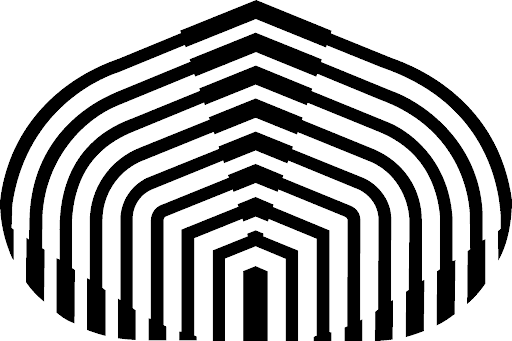
\includegraphics[height = 2cm]{images/logo.png}\\
  \small UNIVERSIDAD SIMÓN BOLÍVAR\\
  DECANATO DE ESTUDIOS PROFESIONALES\\
  COORDINACIÓN DE INGENIERÍA DE COMPUTACIÓN\vspace{3cm}\\
  \LARGE EVALUACIÓN EMPÍRICA DEL CONSUMO ENERGÉTICO Y RENDIMIENTO EN UNA BASE
  DE DATOS DISTRIBUIDA
  \vspace{2.5cm}
}

\author{
  Por:\\
  Lic. Francisco Javier Márquez Hernández\vspace{1.5cm}\\
  \textbf{PROYECTO DE GRADO}\\
  Presentado ante la Ilustre Universidad Simón Bolívar\\
  como requisito parcial para optar al título de\\
  Ingeniero de Computación\\\vspace{0.5cm}
}
\date{Valle de Sartenejas, marzo de 2026}

\addto\captionsspanish{%
  \renewcommand{\tablename}{Tabla}%
  \renewcommand{\chaptername}{Capítulo}%
}

\makeatletter
\renewcommand{\l@chapter}{\@dottedtocline{1}{1.5em}{1.5em}}
\makeatother

\begin{document}
  \maketitle
  {
    \centering
    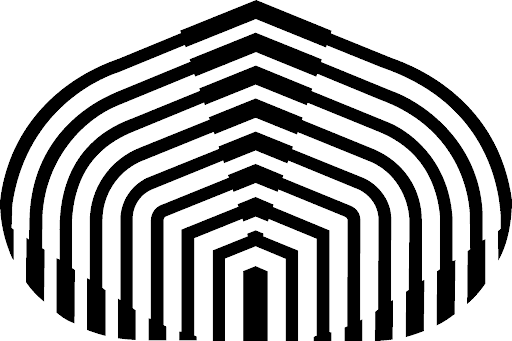
\includegraphics[height = 2cm]{images/logo.png}\\
    UNIVERSIDAD SIMÓN BOLÍVAR\\
    DECANATO DE ESTUDIOS PROFESIONALES\\
    COORDINACIÓN DE INGENIERÍA DE COMPUTACIÓN\vspace{3.5cm}\\
    \LARGE EVALUACIÓN EMPÍRICA DEL CONSUMO ENERGÉTICO Y RENDIMIENTO EN UNA BASE
    DE DATOS DISTRIBUIDA
    \vspace{3.5cm}

    \large Por:\\
    Lic. Francisco Javier Márquez Hernández\vspace{1.5cm}\\
    Realizado con la asesoría de:\\
    Dr. Marlene Goncalves Da Silva\vspace{1.7cm}\\
    \textbf{PROYECTO DE GRADO}\\
    Presentado ante la Ilustre Universidad Simón Bolívar\\
    como requisito parcial para optar al título de\\
    Ingeniero de Computación\\\vspace{1.7cm}

    Valle de Sartenejas, marzo de 2026

    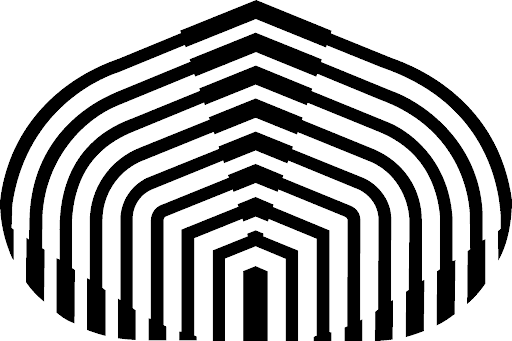
\includegraphics[height = 2cm]{images/logo.png}\\
    \small UNIVERSIDAD SIMÓN BOLÍVAR\\
    DECANATO DE ESTUDIOS PROFESIONALES\\
    COORDINACIÓN DE INGENIERÍA DE COMPUTACIÓN\vspace{2.3cm}\\
    \LARGE EVALUACIÓN EMPÍRICA DEL CONSUMO ENERGÉTICO Y RENDIMIENTO EN UNA BASE
    DE DATOS DISTRIBUIDA
    \vspace{2.3cm}
  
    \large Por:\\
    Lic. Francisco Javier Márquez Hernández\vspace{1.4cm}\\
    Realizado con la asesoría de:\\
    Dr. Marlene Goncalves Da Silva\vspace{1.4cm}\\
    \textbf{RESUMEN}\\
  }
  Aunque la optimización de consultas es crítica, existen escasos estudios que
  evalúen conjuntamente el impacto del diseño físico y el volumen de datos sobre
  el consumo energético en bases de datos relacionales distribuidas. Para
  abordar esta brecha, este trabajo analiza los efectos del uso de índices
  (sugeridos por inteligencia artificial) y la reescritura de consultas sobre el
  gestor PostgreSQL en un entorno distribuido con Citus. La metodología
  contempló la ejecución de consultas del benchmark TPC-H sobre volúmenes de
  datos de entre uno y cincuenta gigabytes. El consumo energético se midió
  mediante Scaphandre, Prometheus e integración numérica, evaluando los planes
  de ejecución a través de correlaciones estadísticas no paramétricas (Kendall y
  Spearman). Los resultados prueban que se puede reducir el consumo energético
  sin dejar de lado una reducción del tiempo de ejecución si se disminuyen las
  operaciones de entrada/salida. Asimismo, los resultados también muestran que
  es posible una degradación del rendimiento y del consumo energético de una
  consulta si no se tiene en consideración las características de la misma al
  momento de hacer el diseño físico.

  \textbf{Palabras clave}: índices, reescritura de consultas, rendimiento,
  TPC-H, consumo energético.

  \newpage
  
  \addcontentsline{toc}{chapter}{\textbf{DEDICATORIA}}
  \begin{center}
    \large \textbf{DEDICATORIA}
  \end{center}

  Dedico este trabajo a:
  Mi madre, quien es incansable en su apoyo durante toda mi carrera.

  Mi pareja, por haberme apoyado en los momentos donde mi propia voluntad
  flaqueaba.

  Mis amigos, Cesar Méndez, Gaby Rodríguez, Andrea Delgado, Jesús Pacheco,
  Samjay Mustafa y Jesus González, quienes insistieron durante años en que
  culminara este proyecto, incluso cuando los múltiples desafíos de Venezuela se
  hacían presentes.

  Mi tutora, Dr. Marlene Goncalves y la profesora Dr. Ana Aguilera, por apoyarme
  en el desarrollo de este proyecto.

  Mi ex-coordinadora de carrera, Dra. Aivlé Cabrera y su asistente, Lic. Gina
  Martínez por tener fe en que iba a culminar mi proyecto.

  Mis estudiantes y exestudiantes Andrea Ceballo, Bárbara Guedes, Franklin
  Camacho, Jean Vásquez, Wismar Pulido, Sofía Gámez, Juan Leandro y Sebastián
  Rodríguez por su apoyo durante momentos difíciles durante este proyecto.

  \newpage
  \addcontentsline{toc}{chapter}{\textbf{AGRADECIMIENTOS}}
  \begin{center}
    \Large \textbf{AGRADECIMIENTOS}
  \end{center}

  Mediante las siguientes líneas quisiera manifestar mi gratitud a:

  Mi madre por su insistencia en mi culminación de este proyecto.

  Mi pareja por su fe en mi éxito.

  Mis profesores por darme la formación que permitió que llevase a cabo este
  proyecto sin más traspiés de los necesarios.

  Mi coordinador por su labor administrativa en el desarrollo de la
  investigación.

  Mi tutora y a la Prof. Ana Aguilera por apoyarme con su experiencia en mis
  experimentos.

  Mis amigos por no permitir que me distrajera de la meta.

  A todos ustedes, en varios idiomas:

  Muchas gracias.

  \textit{Thank you so much.}

  \textit{Merci beaucoup.}

  \begin{CJK}{UTF8}{min}
    \textit{どうもありがとうございます。}
  \end{CJK}

  \tableofcontents
  \addcontentsline{toc}{chapter}{\textbf{Índice general}}

  \newpage
  \addcontentsline{toc}{chapter}{\textbf{Introducción}}
  \begin{center}
    \Large \textbf{Introducción}
  \end{center}

  En los últimos años, con el crecimiento vertiginoso del internet y la
  migración de los sistemas analógicos y físicos hacia sistemas virtuales, se ha
  incrementado el interés por el consumo energético de los centros de datos
  \cite{rongoptimizing2016, maroulisexpress2017}, incluso centrado en las
  técnicas usadas en ellos \cite{florenceenergy2016,
  krzywdapower-performance2018}, y los sistemas gestores de bases de datos
  \cite{bunseenergy2014}. El estudio de la eficiencia de las consultas y su
  consumo energético ha estado presente desde el comienzo, aunque su enfoque ha
  sido más limitado hacia la eficiencia de las consultas sobre bases de datos
  centralizadas \cite{xuexploring2010, langtowards2009, langrethinking2011,
  niemanndoes2013, niemannevaluating2013}. Para los fines de este estudio, el
  término «consulta» trasciende la mera sentencia SQL y se define como el
  proceso holístico e integral que se activa en el sistema: desde la recepción,
  análisis sintáctico y planificación hasta la entrega de los resultados.

  Sin embargo, estos estudios aún requieren mucha más atención a los múltiples
  factores que afectan la eficiencia de las consultas y el consumo energético
  asociado a cada uno: el volumen de datos y el diseño físico. En los estudios
  disponibles, se destaca el efecto energético de las consultas en términos de
  las operaciones elementales de una base de datos (lectura, inserciones,
  eliminaciones y modificaciones). Asimismo, también se estudia cómo operaciones
  de agregación afectan el perfil energético \cite{niemannevaluating2013,
  duarteevaluating2018}. Sobre esa base, se han publicado resultados del consumo
  energético de tales consultas y el efecto que tienen diferentes optimizaciones
  \cite{langrethinking2011, duarteevaluating2018, pisharathreducing2004,
  macdonaldefficient2017, mahajanenergy2017, mahajanimproving2019}. Los trabajos
  consultados coinciden en el estudio de las consultas sin diseño físico y con
  diseño físico, pero restringido sólo al uso de índices. Inclusive, algunos
  \cite{bingleiguosql2015} ponen su enfoque en la manipulacion del planificador
  de consultas ---componente del gestor que se encarga de seleccionar los
  algoritmos y estructuras de ejecución \cite{silberschatz2019database,
  elmasri2016fundamentals, connolly2014database, ramakrishnan2003database}---.
  Por el contrario, la literatura que aborda el impacto de la reescritura de
  consultas es escasa.

  Las investigaciones preliminares reportan un fenómeno contraintuitivo: menores
  tiempos de ejecución pueden generar un mayor consumo energético
  \cite{bingleiguosql2015, guoenergy-efficient2023, bunseexploring2009,
  hopfnertowards2009}. Es contraintuitivo porque la energía consumida por un
  sistema depende de la potencia ---asumida constante--- del mismo y del tiempo
  de trabajo. Así, el incremento del consumo energético por disminución del
  tiempo de ejecución está justificado por la intensificación en el uso del
  hardware y, por tanto, el incremento de la potencia instantánea durante la
  consulta. Al optimizar una consulta, el planificador suele migrar de
  algoritmos de acceso secuencial lentos a mecanismos de procesamiento paralelo
  de alto rendimiento en la CPU. Esta transición suprime los tiempos muertos de
  espera y fuerza a los núcleos del procesador a operar a su máxima frecuencia
  de reloj de forma sostenida. En consecuencia, aunque el intervalo de tiempo
  total ($t$) se reduce, la potencia eléctrica instantánea ($P$) demandada por
  los componentes de la circuitería se incrementa. Como el consumo energético
  ($U$) es la integral de la potencia en el tiempo, si la mejora en rendimiento
  (disminución del tiempo de ejecución) no supera al incremento de la potencia,
  el impacto energético por la mejora no puede ser menor al de la consulta sin
  tal cambio.

  Para cuantificar estos perfiles de consumo, se ha recurrido a herramientas de
  software orientadas a la medición energética de bloques de código en los
  diferentes lenguajes de programación, de los cuales dichas herramientas suelen
  adoptar su nombre (CPPJoules, RJoules, entre otros) \cite{belgaidpyjoules2019,
  chattarajrjoules2023, scppjoules2024, lelladbjoules2023}. No obstante, la
  medición de la eficiencia energética en arquitecturas de datos modernas impone
  el desafío de evaluar entornos distribuidos y coordinados, donde el consumo ya
  no depende de un único hilo de ejecución aislado, sino de la orquestación de
  un clúster de servidores.

  En este sentido, la presente investigación enfoca su marco experimental en un
  ambiente distribuido regido por el gestor de bases de datos PostgreSQL, debido
  a su arquitectura altamente extensible \cite{postgresql_manual} y a su robusto
  ecosistema de extensiones. Como pieza central de esta arquitectura se emplea
  Citus, una extensión que transforma a PostgreSQL en un sistema de bases de
  datos distribuido mediante el particionamiento de tablas (\textit{sharding}) y
  la fragmentación de consultas a través de un clúster de nodos trabajadores y
  un nodo coordinador \cite{citus_paper, citus_docs}. Es debido a la naturaleza
  distribuida del ambiente de trabajo que, la acepción del término <<consulta>>
  de este estudio incluye también planificación en el nodo coordinador de Citus
  incluyendo la fragmentación y ejecución distribuida en los nodos trabajadores,
  hasta la transferencia de red y la consolidación de los resultados en el nodo
  coordinador.

  Para resolver el problema de la medición energética de esta capa distribuida,
  se introduce el uso de Scaphandre como herramienta de monitoreo metrológico de
  bajo nivel basada en el estimador de energía RAPL (\textit{Running Average
  Power Limit}) de Intel y AMD. Scaphandre permite aislar el consumo eléctrico
  ocasionado de forma exclusiva por los identificadores de proceso (PID)
  pertenecientes a PostgreSQL, lo que discrimina el costo energético del gestor
  del resto de procesos del computador \cite{hubblohubblo-orgscaphandre2025}. El
  flujo de estas métricas distribuidas es centralizado en tiempo real por el
  monitor Prometheus, el cual actúa como una base de datos de series temporales
  que recolecta e indexa eficientemente las lecturas de potencia de cada
  instancia de Scaphandre en todos los nodos del clúster de forma síncrona
  \cite{soundcloudoverview2016}.

  La evaluación del comportamiento del clúster ante el estrés computacional se
  realiza mediante las consultas del \textit{benchmark} TPC-H, un estándar de la
  industria compuesto por veintidós consultas de alta complejidad analítica
  diseñadas para apoyo a la toma de decisiones (OLAP). La complejidad de tales
  consultas se pone de manifiesto con operaciones de unión (\texttt{JOIN}) sobre
  varias tablas del esquema TPC-H, subconsultas anidadas correlacionadas,
  agregaciones, ordenamientos y agrupaciones, además de múltiples filtros. TPC-H
  provee un generador de datos aleatorios estandarizado (\texttt{dbgen})
  \cite{transactionprocessingperformancecounciltpctpc2022} para la variación
  controlada del factor de escala del conjunto de datos y la incorporación de la
  escalabilidad vertical en el estudio.

  La investigación se orienta, también, a desentrañar el efecto que poseen las
  estrategias de diseño físico sobre el tiempo de ejecución y consumo de energía
  en arquitecturas distribuidas bajo condiciones de escalamiento vertical.
  Entendidas estas estrategias como la fase culminante del diseño de una base de
  datos dedicada a estructurar el almacenamiento y optimizar los caminos de
  acceso \cite{silberschatz2019database, elmasri2016fundamentals,
  connolly2014database, ramakrishnan2003database}, el estudio se circunscribe
  específicamente a evaluar el uso de índices avanzados y la reescritura de
  consultas SQL. A través de este enfoque empírico, se cuantifica el
  rendimiento ---tiempo de ejecución--- y consumo energético frente a los
  escenarios base (sin diseño físico), y se modela la correlación estadística
  subyacente entre ambas variables, con el fin de determinar si los criterios
  tradicionales de optimización temporal convergen o colisionan con las metas de
  sustentabilidad de la infraestructura. Con este estudio, se desea aportar una
  perspectiva integral sobre cómo las decisiones de diseño físico no solamente
  optimizan el tiempo de respuesta, sino que actúan como un factor determinante
  en la eficiencia energética de los sistemas de bases de datos distribuidas.

  El presente trabajo se estructura de la siguiente manera: en el Capítulo I se
  define el problema de investigación, los antecedentes y los objetivos
  propuestos, cuyas variables operacionales y criterios de evaluación ya han
  sido delimitados conceptualmente en las líneas anteriores. El Capítulo II
  establece el marco teórico y conceptual necesario para el entendimiento del
  hardware y software involucrado, mientras que el Capítulo III describe
  minuciosamente la arquitectura de las herramientas tecnológicas empleadas.
  Posteriormente, el Capítulo IV detalla la metodología, las variables y los
  escenarios experimentales y el Capítulo V expone los resultados obtenidos
  junto con su respectivo análisis. Finalmente, se presentan las conclusiones y
  recomendaciones derivadas de la investigación.

  \chapter{El problema} % (fold)
  \label{cha:el_problema}
    En este capítulo se expondrá el planteamiento del problema de investigación,
    los antecedentes en los que se sustenta esta investigación y los objetivos
    de la misma, los cuales están centrados en el estudio del rendimiento y
    consumo energético del sistema gestor de bases de datos PostgreSQL en un
    entorno distribuido. A tal efecto se emplea el \textit{benchmark} TPC-H
    sobre diversos volúmenes de datos y para los cuales se analizará el tiempo
    de ejecución de las consultas planteadas en él y el consumo energético del
    sistema.

    \section{Planteamiento del problema} % (fold)
    \label{sec:planteamiento_del_problema}
      El consumo energético de los sistemas humanos y la generación de
      alternativas más eficientes ha sido un interés para el mundo desde la
      segunda mitad del siglo XX, cuando aparece la primera gran alerta sobre
      este particular \cite{repashleyhr84441977, horowitzpurchased2014}, y en el
      siglo XXI \cite{murugesangoing2007} se formaliza este interés en los
      procesos informáticos. Los sistemas gestores de bases de datos constituyen
      la columna vertebral de la infraestructura informática actual, impulsada
      por el auge de internet y la virtualización de entornos físicos. Esta
      centralidad ha redirigido el interés hacia la optimización de su
      eficiencia y consumo energético \cite{bunseenergy2014}, un fenómeno
      crítico que impacta tanto a las bases de datos residentes en memoria como
      a las almacenadas en disco.

      Mientras que las bases de datos residentes en memoria (IMDB/MMDB)
      \cite{pisharathreducing2004, nollenergy2017} mitigan el impacto energético
      al operar directamente en la RAM y eliminar la latencia de los cuellos de
      botella de lecturas a disco, las bases de datos en disco ---donde se
      circunscribe esta investigación--- introducen un consumo crítico ligado a
      las operaciones de Entrada/Salida (E/S). Es precisamente en este último
      entorno donde se realizan la mayoría de los estudios disponibles. Dichos
      estudios se realizan bajo el paradigma de optimizar el tiempo de ejecución
      de las consultas, pero algunos trabajos consultados objetan la visión
      sobre el tiempo de ejecución \cite{xuexploring2010, langtowards2009,
      langrethinking2011}.

      El tiempo de ejecución de una consulta en un sistema gestor de bases de
      datos está determinado de forma directa por las decisiones del optimizador
      relacional y la configuración del diseño físico del sistema. El diseño
      físico constituye la fase en la que se definen las estructuras de
      almacenamiento técnico, tales  como los índices avanzados y los mecanismos
      de acceso que permiten al motor localizar los datos sin recurrir a
      costosas lecturas secuenciales de tablas completas
      \cite{silberschatz2019database, elmasri2016fundamentals,
      connolly2014database, ramakrishnan2003database}. A partir de este diseño,
      el optimizador evalúa diferentes planes de ejecución lógicos y selecciona
      los algoritmos que minimicen el costo temporal estimado. Tradicionalmente,
      cualquier alteración en estas estructuras físicas o en la sintaxis de la
      sentencia busca acelerar el procesamiento del motor y se asume que un
      menor tiempo de respuesta equivale a una operación óptima.

      Se han encontrado varios hallazgos como que la disminución del consumo
      energético en las bases de datos al limitar la frecuencia de CPU por
      debajo de su límite máximo \cite{xuexploring2010}. Tales investigaciones
      sugieren que una mejora drástica en tiempo de ejecución de una consulta
      incrementa el consumo energético \cite{langtowards2009} y a su vez, que el
      detrimento en el tiempo de ejecución de una consulta puede conllevar a una
      reducción del consumo energético, lo que contraviene el paradigma
      tradicional de optimización del tiempo de ejecución de las consultas
      \cite{langrethinking2011}.

      Para analizar el comportamiento energético en este ámbito, es imperativo
      descomponer la ejecución de una consulta en sus operaciones constitutivas
      y su contexto transaccional. El procesamiento de una sentencia implica
      tanto operaciones lógicas en la CPU (como filtrados, ordenamientos y
      emparejamientos de datos) como operaciones físicas de E/S para la
      transferencia de páginas desde el almacenamiento. Cuando estas consultas
      forman parte de  un flujo continuo de modificaciones en el estado de la
      base de datos, se agrupan en transacciones ---unidades de trabajo lógico
      que ejecutan operaciones elementales de lectura, inserción, eliminación y
      modificación---. Cada uno de estos subprocesos demanda recursos de
      hardware de manera diferenciada, lo que fragmenta el perfil de potencia
      total del sistema.

      Bajo esta perspectiva operativa, en \cite{langtowards2012} se muestra que
      las operaciones de una consulta pueden estructurarse de forma asimétrica
      en puntos de eficiencia moderada o altamente óptimos, en función de la
      densidad de transacciones concurrentes que saturen el sistema. Sin
      embargo, al mantener una planificación correcta en la asignación de dichas
      operaciones, la potencia demandada se estabiliza en rangos bajos o
      moderados, lo que impacta positivamente en el consumo energético global.

      A su vez, Niemann, en \cite{niemanndoes2013}, encuentra que el consumo
      energético ($U$) y el tiempo de ejecución guardan una correlación lineal
      si y solo si las operaciones de la consulta están atadas puramente al uso
      de la CPU. Por el contrario, cuando intervienen operaciones de E/S
      masivas, esta correlación se rompe, provocando que ejecuciones
      temporalmente más rápidas deriven en una mayor demanda de potencia
      instantánea debido al uso en paralelo de múltiples núcleos de
      procesamiento. Asimismo, en \cite{niemannevaluating2013, 
      duarteevaluating2018} se demuestra que, para lograr una optimización
      energética efectiva, el planificador debe considerar la jerarquía de
      consumo intrínseca  de las operaciones elementales de la transacción,
      donde el gasto energético sigue un orden decreciente bien definido:
      inserciones $\ge$ modificaciones $>$ eliminaciones $\ge$ lecturas.

      Esta escala de consumo se fundamenta en el costo físico y operativo de las
      acciones internas del motor relacional sobre el hardware. Las inserciones
      ocupan la cúspide energética debido a que exigen la asignación de nuevas
      páginas de memoria, la escritura física en el almacenamiento persistente
      y, críticamente, la actualización y rebalanceo en tiempo real de las
      estructuras de indexación \cite{silberschatz2019database,
      elmasri2016fundamentals}, lo que satura de forma simultánea los ciclos de
      CPU y los canales de E/S. Las modificaciones (\textit{updates}) reducen
      levemente este impacto al operar, en ocasiones, sobre registros ya
      asignados, aunque persisten en la exigencia de escritura y reescritura de
      punteros en las páginas de datos \cite{connolly2014database}. Por su
      parte, las eliminaciones suelen ser energéticamente más económicas, ya que
      los gestores frecuentemente ejecutan un borrado lógico mediante el marcado
      de registros  o \textit{tombstones}, postergando la reestructuración
      física del archivo en el disco \cite{ramakrishnan2003database}.
      Finalmente, las lecturas  se ubican en la base de la jerarquía porque
      prescinden por completo de los mecanismos de bloqueo de concurrencia
      pesados y de la costosa persistencia de datos, y se limitan a la
      transferencia de datos que, en entornos optimizados, se resuelve
      directamente a nivel de \textit{buffer cache}
      \cite{silberschatz2019database, elmasri2016fundamentals,
      connolly2014database, ramakrishnan2003database}.

      A pesar del rigor de estos análisis a nivel de operaciones lógicas,
      históricamente el alcance de tales estudios se vio acotado a las bases de
      datos centralizadas, tanto relacionales (MySQL, PostgreSQL, SQLite)
      \cite{xuexploring2010, langtowards2009, langrethinking2011,
      niemanndoes2013, niemannevaluating2013, langtowards2012} como no
      relacionales \cite{duarteevaluating2018, shahcomprehensive2022}. Sin
      embargo, la evolución de las cargas de trabajo impulsó la expansión de
      esta línea de investigación hacia ambientes distribuidos. En
      \cite{foschinisql2023}, se realizan consultas clásicas de bases de datos
      SQL en Cassandra (NoSQL) y se enfrentan problemas propios del cambio de
      paradigma en la arquitectura de los datos. En \cite{gomesenergy2016}, se
      presenta un estudio comparativo entre el consumo energético de bases de
      datos NoSQL con distintos subparadigmas (clave-valor, Redis; documentos,
      MongoDB; columnas, Cassandra). En tal estudio, se encuentra que la
      eficiencia depende, en gran medida, de las condiciones de la carga de
      trabajo. Asimismo, en \cite{gomesnosql-based2023}, se presenta una
      comparación entre los sistemas NoSQL y las implicaciones de cada uno con
      el teorema CAP (\textit{es imposible para un sistema distribuido
      satisfacer simultáneamente consistencia fuerte (C), alta disponibilidad
      (A) y tolerancia a partición (P)} \cite{brewer2000towards,
      gilbert2002brewer}) frente al consumo energético. En
      \cite{songtowards2023}, se caracteriza el consumo con notación asintótica
      para los algoritmos utilizados por los gestores de bases de datos. Estos
      estudios de eficiencia de las consultas y su consumo energético también
      han abarcado el desarrollo de herramientas para apoyar en la medición
      \cite{lellatowards2024, prokhorenkooffloaded2024}.

      En los últimos años, se han empezado estudios sobre los sistemas de bases
      de datos distribuidas \cite{foschinisql2023, gomesnosql-based2023,
      guoenergy2024}. En \cite{subramaniamenergy2015}, se usa Cassandra y el
      tema de la proporcionalidad energética en el aspecto del consumo con
      cargas variables desde la inactividad hasta cargas
      cargas elevadas. Se encontró que, en inactividad, el consumo energético es
      significativo frente al consumo con carga total. También se usa Cassandra
      en \cite{niemanntowards2016}, pero se aborda el tema de la predicción del
      consumo energético y el rendimiento mediante modelos. En
      \cite{roukhenergy-aware2016} se trabaja con PostgreSQL y una herramienta
      propuesta llamada \textit{EnerQuery} y aborda el asunto de la eficiencia
      energética para el caso de una base de datos con un solo nodo con
      múltiples núcleos de CPU. Se encontró que el paralelismo incrementa el
      consumo energético debido al uso de más núcleos a alta frecuencia sin que
      el tiempo de ejecución sea significativamente mayor. Este comportamiento
      fue evaluado en \cite{roukhenergy-aware2016} al implementar una versión
      modificada del optimizador de PostgreSQL en un servidor  con procesador
      Intel Xeon X3430 y 32 GB de RAM; mediante dicha modificación, el gestor
      estimaba analíticamente el costo de potencia basándose en el perfil de los
      operadores SQL y la intensidad de las operaciones de CPU y E/S bajo el
      \textit{benchmark} TPC-H.

      Sin embargo, estos estudios aún requieren mucha más atención a los
      múltiples factores que afectan la eficiencia de las consultas y el consumo
      energético asociado a cada uno \cite{bunseenergy2014}: el volumen de datos
      y el diseño físico. Sobre el volumen de datos, son pocos los estudios que
      dedican poco más de una carga a su base de datos (ver tabla
      \ref{tab:cargas}) y el diseño físico de las bases de datos. Cuando se
      hacen, pueden incluir la reescritura de consultas
      \cite{langrethinking2011, pisharathreducing2004} y el uso de índices
      \cite{duarteevaluating2018, mahajanenergy2017, mahajanimproving2019}.

      \begin{table}[H]
        \centering
        \caption{Volúmenes de datos utilizados frecuentemente}
        \begin{tabular}{| c | c | c | c | c | c | c | c |}
        \hline Volumen (GB) & $<1$ & 1 & 5 & 10 & 25 & 50 & 100 \\ \hline
        Referencias & \cite{pisharathreducing2004, xuexploring2010,
          duarteevaluating2018} & \cite{xuexploring2010, niemanndoes2013} &
          \cite{xuexploring2010, niemanndoes2013} & \cite{xuexploring2010,
          niemanndoes2013, tranenergy2025} & \cite{tranenergy2025} &
          \cite{tranenergy2025}&\cite{mahajanenergy2017, mahajanimproving2019}
                                                                    \\ \hline
        \end{tabular}
        \label{tab:cargas}
      \end{table}

      La literatura actual sobre consumo energético en entornos distribuidos se
      concentra predominantemente en soluciones no relacionales e inherentemente
      distribuidas, como Cassandra y MongoDB \cite{foschinisql2023,
      gomesenergy2016, subramaniamenergy2015}. En contraste, existe una marcada
      escasez de estudios enfocados en sistemas distribuidos relacionales,
      especialmente bajo el efecto de estrategias de diseño físico o ante
      variaciones sistemáticas en el volumen de los datos. Es precisamente esta
      brecha en el estado del arte la que fundamenta la necesidad de ampliar el
      conocimiento disponible sobre este particular, consolidando el espacio de
      estudio de la presente investigación.
    % section planteamiento_del_problema (end)

    \section{Antecedentes} % (fold)
    \label{sec:antecedentes}
      En esta sección se hará una breve descripción de los estudios realizados
      previamente y su relación con la presente investigación. Dichos estudios
      se describirán en dos subsecciones: la concerniente a la eficiencia de las
      consultas y lo relativo a las herramientas que se han usado en el estado
      del arte para la medición del consumo energético.

      \subsection{Eficiencia de las consultas} % (fold)
      \label{sub:eficiencia_de_las_consultas}
        Son numerosos los estudios realizados sobre el comportamiento de las
        consultas a bases de datos relacionales \cite{xuexploring2010,
        langtowards2009, langrethinking2011, niemanndoes2013,
        niemannevaluating2013, pisharathreducing2004, mahajanimproving2019,
        roukhenergy-aware2016} y no relacionales \cite{duarteevaluating2018,
        mahajanenergy2017, mahajanimproving2019, guoenergy-efficient2023,
        shahcomprehensive2022, foschinisql2023, gomesenergy2016,
        gomesnosql-based2023, guoenergy2024, subramaniamenergy2015,
        niemanntowards2016}, ambas en el aspecto energético y el uso de recursos
        del computador. En todos los estudios se destaca el efecto energético de
        las consultas en términos de las operaciones elementales de una base de
        datos (lectura, inserciones, eliminaciones y modificaciones) así como
        operaciones de agregación que solamente usan CPU sin operaciones E/S y
        sobre esa misma base se han publicado resultados sobre el consumo
        energético de tales consultas y el efecto que tienen diferentes
        optimizaciones \cite{langrethinking2011, duarteevaluating2018,
        pisharathreducing2004, macdonaldefficient2017, mahajanenergy2017,
        mahajanimproving2019} sobre dicha variable. Bajo esta misma línea de
        investigación, el enfoque de este estudio está en las bases de datos
        relacionales donde se vinculan estrechamente el desempeño de las
        consultas (tiempo de ejecución) y el consumo energético de cada una
        durante su ejecución en un ambiente distribuido y bajo los efectos de
        una estrategia de diseño físico.

        En este orden de ideas, es fundamental definir la carga de trabajo. En
        diversos estudios previos, se han empleado conjuntos de datos
        heterogéneos como registros de Twitter \cite{mahajanimproving2019},
        usuarios de Netflix y colección de SMS spam \cite{lelladbjoules2023}.
        Otras investigaciones han optado por el uso de pruebas de rendimiento
        estandarizadas, en adelante, \textit{benchmarks}, como:
          \begin{itemize}
            \item Servicios en la nube de Yahoo! (\textit{Yahoo! Cloud Serving
            Benchmark}, YCSB): es un \textit{benchmark} que surge de la  falta
            de herramientas para evaluar y comparar efectivamente sistemas NoSQL
            \cite{cooperbenchmarking2010} y es usado en varios trabajos
            enfocados en trabajos en \textit{la nube} \cite{mahajanenergy2017,
            mahajanimproving2019, gomesenergy2016, subramaniamenergy2015,
            garcia-recueroenergy2016, casalicchioenergy-aware2017}.
            \item \textit{TREC ClueWeb09 category B corpus}
            \cite{macdonaldefficient2017} es un conjunto de datos fundamental
            utilizado en la investigación de recuperación de información y
            tecnologías del lenguaje humano, frecuentemente empleado en las
            conferencias TREC \cite{clueweb09}.
            \item Tienda de DVD de Dell (\textit{Dell DVD Store Benchmark}) es
            una simulación de código abierto de un sitio de comercio
            electrónico en línea con implementaciones en Microsoft SQL Server,
            Oracle, MySQL y PostgreSQL junto con programas controladores y
            aplicaciones web \cite{delltechnologiesindex2010}. Se usó en
            \cite{banistudy2016}.
            \item Tienda de mascotas de Java (\textit{JPetStore Benchmark}): es
            una aplicación web clásica, escrita en Java, que implementa las
            funcionalidades típicas de una tienda en línea (navegación por el
            catálogo, agregar productos al carrito, \textit{login} de usuarios,
            proceso de compra). Utiliza un \textit{backend} de base de datos
            relacional (MySQL, PostgreSQL, etc.) a través del \textit{framework}
            MyBatis \cite{jungjpetstore2018, mybatismybatisjpetstore-62025}. Se
            utilizó en \cite{banistudy2016}.
            \item Procesamiento de transacciones de aplicaciones de
            telecomunicaciones (\textit{Telecom Application Transaction
            Processing Benchmark}, TATP) está diseñado para medir el rendimiento
            de una combinación relacional DBMS/OS/Hardware en una aplicación de
            telecomunicaciones típica (procesamiento de transacciones en línea,
            \textit{On Line Transaction Processing}, OLTP) \cite{wolskitatp2009,
            kissingeradaptive2018}.
            \item Almacén de datos Trabajos de Aventura (\textit{Adventure Works
            Data Warehouse}) es una arquitectura de almacén centralizado que
            consta de tablas de hechos y tablas de dimensiones, y que contiene
            datos obtenidos de la base de datos OLTP y otras fuentes de datos
            mediante un proceso tradicional de extracción/transformación/carga
            \cite{mitriactive2015, mashamsftadventureworks2025} presente en
            \cite{saraivaeconomic2017}.
            \item Suite en la Nube (\textit{CloudSuite Benchmark}): es una suite
            de \textit{benchmarks} para servicios en la nube propios (creados
            por y para la nube). Tiene ocho \textit{benchmarks} que representan
            servicios en línea populares y cargas de trabajo analíticas en
            centros de datos que se basan en pilas de software (conjunto de
            capas de programas que funcionan de manera jerárquica para soportar
            una aplicación o servicio \cite{ferdinandi2012cloudsuite}) de código
            abierto de última generación y están en contenedores para facilitar
            su uso \cite{epflparsacloudsuite2025,
            parsaepflparsa-epflcloudsuite2025}. Fue usado por Subramanian en
            \cite{subramaniamenergy2015-1}.
            \item Consejo de Rendimiento del Procesamiento de Transacciones
            (\textit{Transaction Processing performance Council}, TPC).
            \cite{xuexploring2010, niemanndoes2013, duarteevaluating2018,
            guoenergy-efficient2023, guoenergy2024, tranenergy2025,
            oneilstar2009, poessnew2000, poessenergy2008}.
          \end{itemize}

        Los \textit{benchmarks} OLTP (TATP, JPetStore, Dell DVD Store) están
        diseñados para medir operaciones rápidas y constantes (lecturas simples
        y altas en escritura) \cite{gray1992transaction, difallah2013oltp}. Para
        un estudio de eficiencia energética, las cargas OLTP suelen mantener el
        CPU en estados de uso medio o ráfagas cortas \cite{wood1999dbmss}, lo
        que dificulta la identificación de cuellos de botella energéticos
        complejos. Por su parte, los \textit{benchmark} de enfoque
        NoSQL y Cloud como YCSB y CloudSuite, a pesar de su robustez para un
        sistema distribuido, están diseñados para modelos de datos no
        relacionales y consistencia eventual (modelo donde los nodos convergen a
        un estado común de forma asíncrona si cesan las actualizaciones
        \cite{vogels2009eventually}) \cite{Cooper2010YCSB,
        ferdman2022cloudsuite}. Este estudio está enfocado hacia PostgreSQL por
        lo que un \textit{benchmark} NoSQL no permitiría evaluar el costo
        energético de operaciones críticas como \texttt{JOIN} y también las
        subconsultas anidadas. En el caso de \textit{Adventure Works}
        \cite{Microsoft2023AdventureWorks} y TREC \cite{Voorhees2001Cranfield}, 
        son conjuntos de datos estáticos, es decir, no permiten escalar la
        cantidad de datos de forma controlada y normalizada.

        TPC es un conjunto de \textit{benchmarks} de apoyo de decisión, entre
        los cuales TPC-H destaca como uno de los más utilizados en el ámbito
        académico e industrial
        \cite{transactionprocessingperformancecounciltpctpc2022}. Este
        \textit{benchmark} se compone de veintidós (22) consultas de alta
        complejidad que incorporan funciones de agregación, consultas anidadas,
        operaciones de \texttt{JOIN} masivas. Asimismo, incluye un generador de
        datos variable y normalizado sobre un esquema de ocho (8) tablas que
        emula la lógica de negocio de un entorno corporativo real
        \cite{transactionprocessingperformancecounciltpctpc2022}. Debido
        precisamente a este rigor estructural, a la complejidad algorítmica de
        sus sentencias y a la capacidad de escalar el volumen de información, se
        seleccionó TPC-H como el entorno experimental definitivo para evaluar
        las estrategias de diseño físico en esta investigación.

        Los distintos trabajos consultados coinciden en el estudio de las
        consultas sin diseño físico y con diseño físico (uso de índices) y
        algunos con cambiar configuraciones del planificador de consultas
        (\textit{query planner}). La literatura que considera la reescritura de
        consultas es escasa y reporta que las consultas más eficientes generan
        un mayor consumo de potencia \cite{guoenergy-efficient2023,
        bunseexploring2009, hopfnertowards2009, bingleiguosql2015}.
      % subsection eficiencia_de_las_consultas (end)

      \subsection{Herramientas de medición de consumo} % (fold)
      \label{sub:herramientas_de_medición_de_consumo}
        Se han utilizado numerosas herramientas para la medición del consumo
        energético en operaciones de distinta índole y basados en distintos
        lenguajes de programación: EcoML (basada en Cumulator, que a su vez se
        basa en Python \cite{trebaolcumulator2020}), que es una herramienta para
        registrar la huella de carbono (cantidad de gases de efecto invernadero
        como consencuencia de consumo energético \cite{baldwin2006carbon}) del
        \textit{Machine Learning}, donde se mejoró la estimación del consumo
        energético \cite{igescuecoml2023}; Codecarbon (Python) que estima el
        consumo de potencia eléctrica (GPU, CPU y RAM) y lo aplica a la
        intensidad de carbono de la región donde se lleva a cabo el cómputo
        \cite{mlco2mlco2codecarbon2025}, pyJoules (Python) una herramienta de
        software para medir la huella energética (cantidad total de energía
        consumida por un proceso o actividad \cite{pan2024energy}) de una
        computadora durante la ejecución de un bloque de código de Python.
        Monitorea la energía consumida por dispositivos específicos del
        computador como: socket de CPU Intel, RAM (para servidores de
        arquitectura Intel), GPU Intel integrados (para arquitecturas de
        cliente) y GPU Nvidia \cite{belgaidpyjoules2019}.

        Otras herramientas basadas en otros lenguajes de programación son jRAPL,
        que es un \textit{framework} para perfilar (análisis detallado del
        consumo de recursos de un proceso durante su ejecución
        \cite{pinto2017comprehensive}) programas de Java que se ejecutan en CPU
        compatibles con RAPL (subsección \ref{sub:rapl_y_scaphandre}) funciona
        con cualquier bloque de código de interés energético para el usuario, el
        cual se detecta por estar entre declaraciones del método
        \texttt{EnergyCheck.statCheck()} \cite{kliu20kliu20jrapl2014}. De la
        familia Joules (análogas a pyJoules) se tiene a RJoules y CPPJoules,
        basados en R y C++, respectivamente. RJoules es una interfaz envolvente
        (de los registros de RAPL) desarrollada sobre Intel RAPL que permite el
        registro de trazas de energía directamente desde el sistema operativo
        \cite{chattarajrjoules2023}. CPPJoules utiliza la interfaz
        \texttt{powercap} en Linux para acceder a los datos de consumo
        energético directamente desde varios dominios de Intel-RAPL. Además,
        para la medición de energía de la GPU, CPPJoules utiliza la biblioteca
        NVML9, una API basada en C para supervisar y gestionar varios estados de
        los dispositivos GPU NVIDIA \cite{scppjoules2024}. DBJoules: es una
        herramienta análoga especialmente diseñada para el consumo energético de
        sistemas gestores de bases de datos (DBMS, por sus siglas en inglés)
        \cite{lelladbjoules2023}.

        Como parte de las herramientas orientadas a la evaluación de límites
        térmicos y eléctricos, se destaca el uso de \textit{software} de estrés
        como \texttt{burnMMX}. Este programa, de interfaz de línea de órdenes
        (CLI, por sus siglas en inglés: \textit{Command Line Interface}) y
        perteneciente al paquete \texttt{cpuburn}, está diseñado específicamente
        para someter a la CPU a cargas de trabajo extremas mediante bucles
        infinitos optimizados en lenguaje ensamblador
        \cite{redelmeier2011cpuburn}. A diferencia de otras herramientas del
        conjunto orientadas puramente a las unidades de punto flotante o
        aritméticas, el algoritmo de \texttt{burnMMX} satura intencionalmente
        los buses de comunicación y las interfaces entre la memoria caché y la
        memoria RAM principal en procesadores  con soporte MMX. El propósito de
        este nivel de tensión es forzar el uso sostenido de los controladores de
        memoria a su máxima capacidad, maximizando así la producción de calor y
        la demanda de potencia instantánea de la placa base para evaluar la
        estabilidad del hardware ante picos críticos de consumo
        \cite{redelmeierburnmmx12011}. En el presente trabajo se utilizará
        una herramienta de supervisión de consumo llamada \texttt{Scaphandre}
        que se describirá en la sección \ref{sub:rapl_y_scaphandre}, debido a la
        versatilidad que tiene para trabajar en red y con otras herramientas de
        supervisión centralizada como \texttt{Prometheus}
        \cite{hubblohubblo-orgscaphandre2025}.
      % subsection herramientas_de_medición_de_consumo (end)
    % section antecedentes (end)

    \section{Objetivos} % (fold)
    \label{sec:objetivos}
      \subsection{Objetivo general} % (fold)
      \label{sub:objetivo_general}
        Comparar el rendimiento y el consumo energético en un ambiente
        distribuido, con y sin diseño físico, utilizando el \textit{benchmark}
        TPC-H y el sistema de bases de datos PostgreSQL.
      % subsection objetivo_general (end)

      \subsection{Objetivos específicos} % (fold)
      \label{sub:objetivos_específicos}
        \begin{enumerate}
          \item Determinar el comportamiento del rendimiento\footnote{Tiempo de
          ejecución.} y el consumo energético en el sistema de bases de datos
          PostgreSQL mediante las pruebas de rendimiento TPC-H en un ambiente 
          distribuido sin diseño físico a varios volúmenes de datos.
          \item Caracterizar los parámetros de rendimiento y el consumo
          energético en el sistema gestor de bases de datos PostgreSQL mediante
          las pruebas de rendimiento TPC-H en un ambiente distribuido con diseño
          físico a varios volúmenes de datos.
          \item Comparar el comportamiento del sistema gestor de bases de datos
          PostgreSQL en términos de rendimiento y consumo energético bajo las
          pruebas de rendimiento TPC-H en un ambiente distribuido con y sin
          diseño físico.
          \item Evaluar\footnote{Comparación empírica de las variables medidas
          en el estudio.} el impacto de la estrategia de diseño físico aplicada
          sobre el sistema gestor de bases de datos PostgreSQL mediante
          las pruebas de rendimiento TPC-H en un ambiente distribuido.
        \end{enumerate}
      % subsection objetivos_específicos (end)
    % section objetivos (end)
  % chapter el_problema (end)

  \chapter{Marco teórico} % (fold)
  \label{cha:marco_teórico}
    En el presente capítulo se hablará sobre el \textit{benchmark} utilizado en
    el estudio así como los aspectos teóricos del consumo energético, el diseño
    físico de bases de datos y las pruebas estadísticas que se realizan sobre el
    tipo de datos obtenidos en la investigación.

    \section{\textit{Benchmark} TPC-H} % (fold)
    \label{sec:benchmark_tpc_h}
      El \textit{Transaction Processing Performance Council} (TPC) es una
      organización sin fines de lucro fundada en 1988 con el propósito de
      definir \textit{benchmarks} estandarizados para evaluar el rendimiento de
      entornos de procesamiento de transacciones y bases de datos
      \cite{transactionprocessingperformancecounciltpctpc2022}. Dentro de su
      conjunto de especificaciones, el \textit{benchmark} TPC-H constituye el
      estándar industrial diseñado específicamente para entornos de soporte a la
      toma de decisiones y procesamiento analítico en línea (OLAP). A diferencia
      de las pruebas orientadas a entornos transaccionales (OLTP) que ejecutan
      múltiples operaciones cortas y aisladas, TPC-H ha sido utilizado
      históricamente por la academia y la industria para evaluar la capacidad
      del sistema gestor al procesar grandes volúmenes de datos mediante 
      consultas de alta complejidad algorítmica, examinando la eficiencia de los
      motores frente a un espectro amplio de operadores SQL ejecuciones
      paralelas y accesos intensivos a disco.

      \subsection{Diseño conceptual de la base de datos} % (fold)
      \label{sub:diseño_conceptual_de_la_base_de_datos}
        Para la presente investigación, se usará como \textit{benchmark} a TPC-H
        y en esta sección se describirá brevemente esta herramienta. La base de
        datos del \textit{benchmark} es una simulación de un negocio real y como
        tal, se dará una breve descripción del negocio a efectos de introducir
        la semántica de los elementos de la base de datos. Se indicarán los
        nombres de las relaciones en español en esta descripción discursiva
        junto con su nombre en inglés, que se mantendrá en lo sucesivo para
        efectos de consistencia con la especificación del \textit{benchmark}
        \cite{transactionprocessingperformancecounciltpctpc2022}. El diseño
        lógico de la base de datos se presenta en el apéndice \ref{apx:tpch}.\\

        En una nación (\texttt{nation}), la cual está localizada en una región
        (\texttt{region}), hay clientes (\texttt{customer}) que realizan
        pedidos (\texttt{orders}) y proveedores (\texttt{supplier}) que
        suministran partes (\texttt{part}) para satisfacer los pedidos que
        están en una línea de artículos (\texttt{lineitem}). Cada
        \texttt{region} y \texttt{nation} se caracterizan por su nombre
        (\texttt{name}), un comentario (\texttt{comment}) y un código único
        (\texttt{key}).


        Las \texttt{part} tienen su \texttt{key}, \texttt{name},
        \texttt{comment}, fabricante (\texttt{mfgr}), marca (\texttt{brand}),
        tipo (\texttt{type}), tamaño (\texttt{size}), precio al detal
        (\texttt{retailprice}) y contenedor (\texttt{container}). Los
        \texttt{supplier} tienen su \texttt{name}, dirección (\texttt{address}),
        teléfono (\texttt{phone}), saldo en su cuenta (\texttt{acctbal}), su
        \texttt{comment} y \texttt{key}. Se entiende que varios
        \texttt{supplier} pueden suministrar la misma \texttt{part}, aunque su
        disponibilidad (\texttt{availqty}) y su costo (\texttt{supplycost})
        varían según \texttt{supplier} y \texttt{part} y pueden tener un
        \texttt{comment}.


        Los \texttt{customer} comparten las características de los
        \texttt{supplier}, pero agregan un segmento de mercado
        (\texttt{mktsegment}). Las \texttt{orders} también tienen su
        \texttt{key} y \texttt{comment} y estado (\texttt{status}), monto total
        facturado (\texttt{totalprice}), fecha de solicitud
        (\texttt{orderdate}), prioridad (\texttt{orderpriority}), empleado
        (\texttt{clerk}), prioridad de envío (\texttt{shippriority}); mientras
        que las \texttt{lineitem} se identifican unívocamente por la orden y el
        número de línea (\texttt{linenumber}) y también contienen cantidad
        (\texttt{quantity}), precio bruto (\texttt{extendedprice}), descuento
        (\texttt{discount}), impuesto (\texttt{tax}), advertencia
        (\texttt{returnflag}), estado de la línea (\texttt{linestatus}), fecha
        acordada (\texttt{commitdate}) y de entrega (\texttt{receiptdate}),
        instrucción de envío (\texttt{shipinstruct}), modo de envío
        (\texttt{shipmode}) y su \texttt{comment}.

        Finalmente, se presenta el diagrama entidad-relación simplificado sin
        atributos para ilustrar el diseño conceptual de la base de datos en la
        figura \ref{fig:ER}.

        \begin{figure}[H]
          \centering
          \begin{tikzpicture}[node distance=5em]
            \node[entity] (r) {REGION};
            \node[relationship] (bto) [left of=r]{\tiny Belongs to} edge (r);
            \node[entity] (n) [below of=bto] {NATION} edge (bto);
            \node[relationship] (ctzn) [right of=n] {\tiny is} edge (n);
            \node[entity] (cust) [right of=ctzn] {CUSTOMER} edge (ctzn);
            \node[relationship] (plcs)[below of=cust]{\tiny Places}edge(cust);
            \node[entity] (o) [below of=plcs] {ORDERS} edge (plcs);
            \node[relationship] (cons) [left of=o]{\tiny Constitutes}edge (o);
            \node[entity] (l) [left of=cons] {LINEITEM} edge (cons);
            \node[relationship] (sto) [left of=n] {\tiny Supplies to}edge (n);
            \node[entity] (supp) [below of=sto] {SUPPLIER} edge (sto);
            \node[relationship] (psup) [left of=l] {\tiny Partsupp} edge (l) edge (supp);
            \node[entity] (part) [left of=psup] {PART} edge (psup);
          \end{tikzpicture}
          \caption{Diagrama Entidad Relación simplificado sin atributos}
          \label{fig:ER}
        \end{figure}
      % subsection diseño_conceptual_de_la_base_de_datos (end)

      \subsection{Consultas} % (fold)
      \label{sub:consultas}
        El \textit{benchmark} consta de veintidós consultas (Q1..Q22), cuya
        descripción detallada y su implementación se presenta en el apéndice
        \ref{apx:tpch}.

        En la tabla \ref{tab:queries} donde se comparan las consultas del
        \textit{benchmark} en términos del número total de operaciones de
        \texttt{JOIN} de la consulta (\texttt{JOIN} totales), funciones de
        agregación aplicadas (agregaciones), niveles de anidamiento, tipo de
        operaciones (Operaciones; S para \texttt{SELECT}, C para \texttt{CREATE}
        y D para \texttt{DELETE}) y agrupamientos.

        En la tabla \ref{tab:queries} se mencionan varios tipos de \texttt{JOIN}
        así que, se procederá a definirlos. Primeramente, el Semi JOIN es una
        operación en álgebra relacional y bases de datos que devuelve las tuplas
        de una relación izquierda (R) para las cuales existe al menos una tupla
        coincidente en la relación derecha (S), basándose en una condición de
        combinación (C). Se diferencia del \texttt{JOIN}, porque no duplica las
        filas de R si hay múltiples coincidencias en S, ni extrae las columnas
        de S. Su propósito algorítmico es estrictamente el filtrado por
        existencia. En cuanto el motor encuentra la primera coincidencia en S
        para una tupla de R, detiene la búsqueda para esa tupla (evaluación de
        cortocircuito) y la incluye en el resultado
        \cite{silberschatz2019database}. Formalmente en álgebra relacional,
        se define como la proyección de los atributos de R sobre el
        \texttt{JOIN} de R y S como se indica en (\ref{eq:semijoin}) y se
        implementa en SQL con \texttt{EXISTS} o \texttt{IN}

        Por su parte, el \texttt{LEFT OUTER JOIN} es una operación relacional
        que preserva toda la información de R, independientemente de si existe
        una coincidencia en S. El resultado de esta operación incluye todas las
        tuplas que se generarían en un \texttt{JOIN} más aquellas tuplas de R
        que no cumplen la condición de combinación con ninguna tupla de S. Para
        estas tuplas sin coincidencia (\textit{dangling tuples}), los atributos
        de S correspondientes se rellenan con valores nulos (\texttt{NULL}).
        Algorítmicamente, impide la propiedad conmutativa del optimizador de
        consultas, ya que el orden lógico de la retención de datos está fijado
        hacia la relación declarada a la izquierda
        \cite{elmasri2016fundamentals}.

        \begin{equation}
          R \ltimes_{C} S = \pi_{atributos(R)}(R \bowtie S)
          \label{eq:semijoin}
        \end{equation}

        \begin{table}[H]
          \centering
          \begin{threeparttable}
          \caption{Resumen de las implementaciones de las consultas}
          \begin{tabular}{| c | c | c | c | c | c |}
            \hline
            Consulta        & \texttt{JOIN} totales & Agregación & Niveles de anidamiento & Operaciones & Agrupamientos \\ \hline
                Q1          &           0           &      8     &            0           &       S     &       2       \\ \hline
                Q2          &         4 + 3         &      1     &            1           &       S     &       0       \\ \hline
                Q3          &           2           &      1     &            0           &       S     &       3       \\ \hline
                Q4          &         $1^b$         &      1     &            1           &       S     &       1       \\ \hline
                Q5          &           5           &      1     &            0           &       S     &       1       \\ \hline
                Q6          &           0           &      1     &            0           &       S     &       0       \\ \hline
                Q7          &           5           &      1     &            1           &       S     &       3       \\ \hline
                Q8          &           7           &      2     &            1           &       S     &       1       \\ \hline
                Q9          &           5           &      1     &            1           &       S     &       2       \\ \hline
               Q10          &           3           &      1     &            0           &       S     &       7       \\ \hline
               Q11          &         2 + 2         &      3     &            1           &       S     &       1       \\ \hline
               Q12          &           1           &      2     &            0           &       S     &       1       \\ \hline
               Q13\tnote{a} &         $1^c$         &      2     &            1           &       S     &       2       \\ \hline
               Q14          &           1           &      2     &            0           &       S     &       0       \\ \hline
               Q15          &           1           &      2     &            1           &      CSD    &       1       \\ \hline
               Q16\tnote{a} &       $1 + 1^d$       &      1     &            1           &       S     &       3       \\ \hline
               Q17          &       $1 + 1^b$       &      2     &            1           &       S     &       0       \\ \hline
               Q18          &       $2 + 1^b$       &      2     &            1           &       S     &       5       \\ \hline
               Q19          &           1           &      1     &            1           &       S     &       0       \\ \hline
               Q20\tnote{a} &     $1 + 1^b + 2$     &      1     &            2           &       S     &       0       \\ \hline
               Q21          &    $3 + 1^b + 1^d$    &      1     &            1           &       S     &       1       \\ \hline
               Q22          &         $1^d$         &      5     &            2           &       S     &       1       \\ \hline
          \end{tabular}
          \label{tab:queries}
          \begin{tablenotes}
            \item[a] La consulta tiene coincidencia de patrones (\textit{pattern matching}).
            \item[b] Es un \texttt{SEMI JOIN}.
            \item[c] Es un \texttt{LEFT OUTER JOIN}.
            \item[d] Es un \texttt{ANTI JOIN}.
          \end{tablenotes}
          \end{threeparttable}
        \end{table}

        El \texttt{ANTI JOIN} es una operación lógica de filtrado que devuelve
        las tuplas de R para las cuales no existe ninguna tupla coincidente en S
        bajo una condición específica, C. Es el complemento lógico del
        \texttt{SEMI JOIN}. Algorítmicamente, el motor de la base de datos toma
        una tupla de R y la evalúa contra S. Si encuentra aunque sea una
        coincidencia, la tupla de R es inmediatamente descartada. Si recorre las
        opciones en S y confirma la ausencia absoluta de coincidencias, la tupla
        de R es enviada al conjunto de resultados. Al igual que el \texttt{SEMI
        JOIN}, no proyecta atributos de la tabla derecha. Formalmente, se
        expresa como la diferencia de conjuntos entre la relación completa R y
        el \texttt{SEMI JOIN} de R y S como se indica en (\ref{eq:antijoin}) y
        se implementa en SQL con \texttt{NOT EXISTS} o \texttt{NOT IN}
        \cite{garcia2009database}.

        \begin{equation}
          R \triangleright_{C} S = R - (R \ltimes_{C} S)
          \label{eq:antijoin}
        \end{equation}
      % subsection consultas (end)
    % section benchmark_tpc_h (end)

    \section{Medición del consumo energético} % (fold)
    \label{sec:medición_del_consumo_energetico}
      \subsection{Potencia eléctrica} % (fold)
      \label{sub:potencia_eléctrica}
        Por definición, potencia es el trabajo realizado por un sistema en una
        unidad de tiempo. Para intervalos de tiempo ($dt$) infinitesimales se
        tiene que la fuerza eléctrica ($\vec{F}_e$) hace trabajo para hacer que
        los portadores de carga se desplacen una cantidad $d\vec{r}$ por lo que
        se cumple (\ref{eq:potencia}):

        \begin{equation}
          P = \dfrac{d}{dt} \int{\vec{F}_e \cdot d\vec{r}}
          \label{eq:potencia}
        \end{equation}

        Y se puede demostrar (\ref{eq:potenciaElectrica}), donde $\Delta V$ es
        la diferencia de potencial entre los dos puntos donde ocurre el
        desplazamiento total de la carga e $i$ la corriente asociada al
        movimiento de los portadores de carga \cite{sears2004fisica}.

        \begin{equation}
          P = i \Delta V
          \label{eq:potenciaElectrica}
        \end{equation}

        Al trasladar este principio físico a la escala nanométrica de los
        circuitos integrados modernos, como los microprocesadores que equipan a
        los servidores, la potencia total demandada por el circuito se
        manifiesta y divide principalmente en dos componentes operacionales: la
        potencia estática y la potencia dinámica. La potencia estática
        representa la energía disipada de forma continua por fugas de corriente
        en los transistores mientras el circuito se encuentra energizado pero en
        estado de inactividad (\textit{idle}). Por el contrario, la potencia
        dinámica constituye la energía consumida directamente por la conmutación
        activa de los transistores al cambiar de estado lógico para ejecutar
        instrucciones de CPU.

        Como la tasa de conmutación de estos millones de transistores varía
        milisegundo a milisegundo en función del tipo de instrucciones que
        procesa el sistema operativo, la potencia eléctrica de un computador no
        puede ser concebida como una variable estática o un valor constante. Por
        el contrario, se comporta como una función matemática sumamente volátil
        que fluctúa en tiempo real según la intensidad de la carga de trabajo
        impuesta al hardware. En la práctica computacional, esto implica que
        cualquier intento de cuantificar la demanda eléctrica de un proceso de
        software no arrojará un resultado fijo, sino una serie temporal de
        lecturas discretas y altamente variables. Por lo tanto, la determinación
        de la energía total derivada de esta potencia evita los cálculos
        algebraicos tradicionales y exige un tratamiento acumulativo en el
        tiempo, abriendo las puertas al uso de la integración y los métodos 
        numéricos para consolidar dichas fluctuaciones.
      % subsection potencia_eléctrica (end)

      \subsection{Consumo energético} % (fold)
      \label{sub:consumo_energetico_teorico}
        El consumo energético ($U$) es, por la misma definición de potencia
        ($P$), la acumulación de la energía demandada a lo largo de un periodo
        de ejecución, lo cual se expresa formalmente mediante la ecuación
        (\ref{eq:consumo}), donde $t$ representa el intervalo temporal que toma
        realizar el traslado de los portadores de carga \cite{sears2004fisica}.

        \begin{equation}
          U = \int_{t_0}^{t_f} P(t) dt
          \label{eq:consumo}
        \end{equation}

        En tal sentido, el consumo energético puede calcularse mediante métodos
        numéricos como la regla del trapecio (donde se aproxima la potencia
        como segmentos de recta separados a intervalos regulares)
        \cite{burden2010numerical}. Esta aproximación responde a que las
        arquitecturas actuales de hardware implementan contadores de rendimiento
        y sensores de energía  internos integrados (como los módulos de
        telemetría digital de los procesadores modernos). Estos sensores
        realizan un muestreo discreto de las  variables eléctricas a altas
        frecuencias y digitalizan el comportamiento de la potencia para entregar
        métricas en intervalos de tiempo fijos y regulares.
      % subsection consumo_energetico_teorico (end)
    % section medición_del_consumo_energetico (end)

    \section{Diseño físico de bases de datos} % (fold)
    \label{sec:diseño_físico_de_bases_de_datos}
      El diseño físico de una base de datos es la etapa final
      \cite{connolly2014database} del proceso de diseño, donde el esquema lógico
      (tablas, relaciones y restricciones) se traduce en una implementación real
      \cite{silberschatz2019database, elmasri2016fundamentals,
      connolly2014database} dentro de un gestor de base de datos. Es un
      proceso continuo centrado en el entendimiento de la carga de trabajo, la
      selección de estrategias y el ajuste posterior a la selección hasta que
      se alcanza un rendimiento aceptable para el administrador de la base de
      datos \cite{ramakrishnan2003database}. Dentro de las estrategias que se
      pueden implementar para el diseño físico están: el uso de índices y la
      reescritura de consultas. Desde la perspectiva de la eficiencia
      energética, estas estrategias permiten reducir el número de páginas de
      disco leídas y los ciclos de CPU invertidos, disminuyendo de forma directa
      la potencia dinámica del hardware. Dentro de las líneas de acción con
      mayor impacto que se pueden implementar para el diseño físico están el uso
      de índices y la reescritura de consultas.

      \subsection{Índices} % (fold)
      \label{sub:índices}
        Son estructuras auxiliares de datos que aceleran la recuperación de la
        información en la base de datos \cite{silberschatz2019database,
        elmasri2016fundamentals, connolly2014database,
        ramakrishnan2003database}. Como estructuras, los índices suelen ser
        \textit{B-Tree} por árbol balanceado (\textit{balanced tree}) con tiempo
        de búsqueda logarítmico \cite{silberschatz2019database} y recomendado
        para lecturas por rango \cite{ramakrishnan2003database}, es decir,
        consultas donde se usen operadores de desigualdad o \texttt{BETWEEN} (en
        SQL). Y también se suelen usar índices de \textit{Hash} (una
        implementación particular de tablas de \textit{hash} para gestores de
        bases de datos), recomendados para búsquedas por igualdad
        \cite{elmasri2016fundamentals}, pero no para búsquedas por rango
        \cite{connolly2014database}.

        Hay especializaciones, como los \textit{B+ Trees}, que optimizan a los
        \textit{B Trees} al unir cada hoja del árbol y formar una lista
        enlazada lo que hace que las búsquedas por rangos sean aún más rápidas
        en la práctica \cite{ramakrishnan2003database}. Sin embargo, aún estos
        índices presentan limitaciones de búsqueda para un caso particular:
        atributos de texto. Para ello se tienen los índices \textit{Full Text}
        que funcionan como el índice analítico (o alfabético) de los libros:
        en estos índices cada palabra es almacenada junto con apuntadores a
        cada lugar donde aparece \cite{silberschatz2019database,
        ramakrishnan2003database, manning2008introduction}.

        Dentro de este tipo de índices, PostgreSQL ofrece una implementación de
        gran interés para la presente investigación: los índices de trigramas
        GIN \cite{silberschatz2019database, elmasri2016fundamentals,
        ramakrishnan2003database}. Este mecanismo, en lugar de guardar palabras
        completas, descompone las cadenas de texto y almacena solamente
        subcadenas de tres caracteres (trigramas), lo que acelera notablemente
        la búsqueda de patrones con el operador \texttt{LIKE} al reducir el
        esfuerzo de procesamiento. Para los fines de este trabajo, se utilizarán
        las estructuras \textit{B+ Trees} (por ser el estándar por defecto de
        PostgreSQL) y GIN de trigramas, con el objetivo de evaluar cómo la
        elección de cada uno de estos caminos de acceso afecta el rendimiento
        temporal y el perfil de consumo energético del sistema.
      % subsection índices (end)

      \subsection{Reescritura de consultas} % (fold)
      \label{sub:reescritura_de_consultas}
        En primera instancia, el gestor de bases de datos no ejecuta las
        consultas como están escritas en el lenguaje de alto nivel, sino que
        primero son optimizadas por el gestor de bases de datos antes de
        ejecutarlas \cite{silberschatz2019database}. Por otro lado, la forma
        en la que se plantea la consulta le impide al gestor hacer una buena
        optimización o incluso, decidir si usa un índice o no (por ejemplo,
        usar solamente el año en un filtro en lugar de un rango: con este
        último, el gestor sí usa el índice) \cite{ramakrishnan2003database}.

        El proceso de reescritura de consultas no es necesariamente sencillo y
        en muchos casos puede llegar a alterar la lógica de la consulta y, por
        tanto, el resultado de la misma, por lo tanto, se debe avanzar con
        cautela por esta vía \cite{ramakrishnan2003database,
        chaudhuri1998overview, date2012database}. En el caso de esta
        investigación, la reescritura de consultas será puntual al usar copias
        de una tabla que está distribuida por otro atributo.
      % subsection reescritura_de_consultas (end)

      \subsection{Expresiones de tabla común (CTE)} % (fold)
      \label{sub:expresiones_de_tabla_comun_cte}
        Una expresión de tabla común (CTE, por sus siglas en inglés,
        \textit{Common Table Expression}) se define formalmente como un conjunto
        de resultados temporales y con nombre, el cual se deriva de una consulta
        relacional y cuyo ciclo de vida (y alcance de ejecución) está
        restringido exclusivamente a una única instrucción principal
        (\texttt{SELECT}, \texttt{INSERT}, \texttt{UPDATE} o \texttt{DELETE}).

        Fueron incluidas formalmente en el estándar SQL:1999 (también conocido
        como SQL3) a través de la cláusula \texttt{WITH}, las CTE actúan
        conceptualmente como vistas efímeras (o tablas derivadas \textit{in
        line}). Su importancia en la arquitectura de consultas radica en dos
        propiedades fundamentales: la modularidad y reusabilidad algorítmica; y
        la recursividad (semántica de punto fijo). La modularidad y reusabilidad
        permiten descomponer consultas analíticas complejas en bloques lógicos
        secuenciales. A diferencia de las subconsultas anidadas tradicionales,
        una CTE puede ser referenciada múltiples veces dentro de la misma
        instrucción principal sin necesidad de reescribir la lógica ni persistir
        los datos físicamente en el disco. La recursividad, a través de la
        variante \texttt{WITH RECURSIVE}, dotó al lenguaje SQL de la capacidad
        matemática de procesar grafos y estructuras jerárquicas de profundidad
        arbitraria. Esto se logra evaluando iterativamente un miembro ancla
        (caso base) y un miembro recursivo uniéndolos hasta que no se produzcan
        nuevas tuplas \cite{silberschatz2010database}.

        \subsubsection{Materialización} % (fold)
        \label{ssub:materialización}
          La materialización se define como el proceso de evaluar una expresión
          relacional (como una vista, una subconsulta o una CTE) y almacenar
          físicamente su conjunto resultante de tuplas en una estructura de
          datos temporal o persistente, en lugar de recalcular dichos resultados
          al vuelo (\textit{on the fly} o \textit{pipelining}) cada vez que son
          referenciados por una consulta externa. Conceptualmente, esto es la
          aplicación directa del principio de intercambio entre espacio y
          tiempo: se sacrifica espacio de almacenamiento (disco o memoria) y
          frescura de los datos a cambio de una reducción drástica en el costo
          computacional (CPU e I/O) durante el tiempo de lectura. Se implementa
          en SQL con \texttt{MATERIALIZED} \cite{ramakrishnan2003database}.
        % subsubsection materialización (end)
      % subsection expresiones_de_tabla_comun_cte (end)
    % section diseño_físico_de_bases_de_datos (end)

    \section{Gestión de memoria} % (fold)
    \label{sec:gestión_de_memoria}
      La ejecución de consultas complejas sobre un gestor de bases de datos no
      depende únicamente de la eficiencia algorítmica de su diseño lógico o
      físico, sino que está profundamente condicionada por la interacción entre
      el gestor de la base de datos, el sistema operativo y la infraestructura
      de hardware subyacente. Para comprender cómo escala el rendimiento y el
      consumo energético ante variaciones drásticas en el volumen de datos, es
      fundamental analizar los fenómenos físicos y operativos que ocurren
      durante la transferencia de información entre los diferentes niveles de
      almacenamiento \cite{silberschatz2019operating}.

      En esta sección se abordan los fundamentos de la administración de la
      memoria principal mediante el espacio de almacenamiento temporal del
      gestor, el impacto de los patrones de consulta desestructurados sobre la
      eficiencia del hardware, y las consecuencias del desbordamiento de la
      memoria de trabajo a través de los mecanismos de transferencia hacia el
      almacenamiento persistente.

      \subsection{Jerarquía de memoria y administración del \textit{buffer pool}} % (fold)
      \label{sub:jerarquía_de_memoria_y_administración_del_buffer_pool}
        La arquitectura de un servidor moderno está gobernada por una pirámide
        jerárquica de almacenamiento. En la cúspide se ubican los componentes
        más cercanos al procesador (las memorias caché L1, L2 y L3), las cuales
        ofrecen latencias de acceso extremadamente bajas pero capacidades de
        almacenamiento muy reducidas. Inmediatamente abajo se encuentra la
        memoria de acceso aleatorio (RAM) y, finalmente, en la base se sitúa el
        almacenamiento secundario o persistente (unidades de estado sólido o
        discos mecánicos), caracterizado por poseer capacidades masivas a costa
        de tiempos de respuesta exponencialmente mayores.

        En este entorno, los DBMS implementan un componente crítico de software
        denominado \textit{buffer pool} o administrador de búferes. El
        \textit{buffer pool} es una región de la memoria RAM reservada
        explícitamente por el gestor de la base de datos para almacenar
        temporalmente las páginas de datos y de índices que se leen desde el
        almacenamiento persistente. El objetivo primordial de este mecanismo es
        minimizar las operaciones físicas de E/S, aprovechando el principio de
        localidad espacial y temporal de las consultas para resolver la mayor
        cantidad de peticiones directamente en los componentes circuitales
        rápidos \cite{ramakrishnan2003database}.

        Cuando el gestor de evaluación de consultas requiere procesar un
        dconjunto e registros, el administrador de búferes verifica si las
        páginas solicitadas ya residen en la memoria principal, un fenómeno
        conocido como \textit{buffer hit}. En ese caso, el acceso a los datos se
        realiza de forma casi instantánea a la velocidad nativa de la RAM, o
        incluso de las memorias caché de la CPU si el volumen de datos es lo
        suficientemente compacto como para ser retenido en los registros del
        procesador.

        Por el contrario, si las páginas no se encuentran en memoria se produce
        un \textit{buffer miss}, lo que obliga al gestor a suspender
        momentáneamente la operación en la CPU para emitir una solicitud de
        lectura física al almacenamiento secundario \cite{tanenbaum2014modern}.
        Debido a que el costo temporal de leer desde el disco es de varios
        órdenes de magnitud superior al de la memoria RAM, la tasa de aciertos
        del \textit{Buffer Pool} se convierte en el factor determinante del
        rendimiento general de la base de datos \cite{ramakrishnan2003database}.

        Cuando el tamaño de las tablas de un esquema de base de datos escala y
        supera la capacidad física asignada al \textit{buffer pool}, el espacio
        de memoria se satura. Ante un \textit{buffer miss}, en este escenario,
        el gestor no puede cargar la nueva página sin antes desalojar una
        preexistente. Para ello, los gestores implementan políticas de reemplazo
        de páginas como el algoritmo \textit{Least Recently Used} (LRU)
        \cite{ramakrishnan2003database}. Este algoritmo identifica y expulsa la
        página que lleva más tiempo sin ser consultada; sin embargo, si la carga
        de trabajo exige una lectura secuencial masiva que supera el tamaño del
        búfer, LRU se vuelve ineficiente, provocando un ciclo infinito de
        desalojos y cargas físicas. Este fenómeno marca el inicio de la
        degradación drástica del rendimiento, trasladando el cuello de botella
        desde la lógica del software hacia las restricciones físicas del
        hardware de almacenamiento.
      % subsection jerarquía_de_memoria_y_administración_del_buffer_pool (end)

      \subsection{Tormenta de accesos aleatorios} % (fold)
      \label{sub:tormenta_de_accesos_aleatorios}
        Las técnicas de diseño físico descritas en las subsecciones anteriores
        tienen como propósito fundamental mitigar el impacto adverso de los
        patrones de acceso ineficientes al almacenamiento secundario. De acuerdo
        con \cite{hellerstein2007architecture}, el motor de ejecución de un
        sistema gestor de bases de datos opera bajo una arquitectura donde el
        subsistema de Entrada/Salida (E/S) representa el principal cuello de
        botella, dado que las operaciones para recuperar páginas de datos desde
        el almacenamiento hacia el \textit{buffer pool} de la memoria RAM son
        órdenes de magnitud más lentas que los ciclos de procesamiento de la CPU
        \cite{hellerstein2007architecture}.

        La tormenta de accesos aleatorios es una condición de saturación crítica
        en el subsistema de almacenamiento. Este fenómeno se caracteriza por la
        ejecución masiva y concurrente de operaciones sobre bloques de datos que
        no guardan contigüidad física en el disco. Esta dispersión de
        solicitudes hacia bloques de datos no contiguos desencadena la patología
        en el hardware que satura críticamente las colas de E/S. Al no
        implementarse estructuras de acceso físico que agrupen u ordenen la
        ubicación de los datos en el disco, la controladora de almacenamiento
        colapsa bajo el peso de miles de peticiones de lectura pequeñas y
        arbitrarias que compiten entre sí por los recursos de transferencia.

        La consecuencia directa de este escenario no es solo una degradación
        exponencial del rendimiento temporal del DBMS, sino también un
        incremento drástico en la demanda de potencia eléctrica y el consumo
        energético del hardware de almacenamiento, el cual debe operar a su
        máxima capacidad de transferencia para resolver un mapa caótico de
        direccionamiento físico \cite{graefe1993query,
        hellerstein2007architecture}. Así, la tormenta de accesos aleatorios se
        consolida como el principal enemigo de la eficiencia energética en el
        software de bases de datos lo que justifica la necesidad de implementar
        estrategias de optimización física que transformen el acceso aleatorio
        concurrente en lecturas ordenadas y predecibles.
      % subsection tormenta_de_accesos_aleatorios (end)

      \subsection{Mecanismos de paginación y fallos de página} % (fold)
      \label{sub:mecanismos_de_paginación_y_fallos_de_página}
        La eficiencia de las estructuras de diseño físico, particularmente de
        los índices densos, depende críticamente de la velocidad del sustrato de
        hardware donde residen durante la ejecución de las consultas. Los
        sistemas operativos modernos gestionan la memoria a través de un esquema
        de memoria virtual, el cual abstrae el almacenamiento físico en bloques
        de tamaño uniforme denominados páginas \cite{silberschatz2019operating}.
        El gestor de la base de datos confía en que las páginas que contienen
        los nodos del índice se encuentren alojadas en la RAM para garantizar
        tiempos de respuesta en el orden de los microsegundos
        \cite{elmasri2015fundamentals}.

        Sin embargo, cuando el volumen de los datos o el tamaño acumulado de las
        estructuras auxiliares indexadas excede la capacidad de la memoria
        asignada al buffer del gestor, la unidad de gestión de memoria (MMU por
        sus siglas en inglés) se ve imposibilitada para resolver las direcciones
        lógicas de forma nativa \cite{tanenbaum2014modern}. Al intentar acceder
        a una sección del índice que no se encuentra cargada físicamente en la
        memoria, el sistema operativo interrumpe el hilo de procesamiento y
        genera una excepción de hardware denominada fallo de página
        (\textit{page fault}), específicamente un fallo de página mayor
        (\textit{major page fault}) \cite{silberschatz2019operating}. A
        diferencia de un fallo menor (\textit{minor page fault}) ---donde la
        página ya reside en la RAM y solo requiere una reasignación de punteros
        a nivel de software---, el \textit{major page fault} obliga al sistema
        operativo a suspender la ejecución del proceso de la consulta en la CPU
        para realizar una operación de lectura física en el almacenamiento
        secundario, y trasladar la página faltante desde el disco hacia la RAM.

        La ocurrencia de un \textit{major page fault} altera drásticamente el
        perfil de consumo energético a través de tres mecanismos de bajo nivel.
        En primer lugar, se genera un escenario de sincronización y
        conmutación a un estado inactivo en la CPU, donde el procesador debe
        suspender la ejecución del hilo de la consulta SQL y ceder los ciclos
        de reloj al kernel del sistema operativo para que este programe la
        operación de E/S. Dado que las pruebas se realizan en un entorno de
        servidor dedicado exclusivo para el DBMS, al bloquearse la consulta la
        cola de procesos listos de usuario queda vacía; en consecuencia, la CPU
        se ve obligada a conmutar hacia el proceso inactivo del sistema
        (\textit{idle}), entrando en un estado de baja potencia por inactividad
        donde consume energía basal sin avanzar en el cálculo de la consulta
        \cite{niemann2012}. En segundo lugar, ocurre la activación del
        almacenamiento secundario, donde el controlador de almacenamiento debe
        localizar y transferir la página faltante desde el soporte físico hacia
        la RAM \cite{elmasri2015fundamentals}. Esta activación tanto del bus de
        datos como de los circuitos integrados de la memoria secundaria dispara
        la demanda de potencia eléctrica del componente de almacenamiento, un
        impacto energético que ha sido documentado al evaluar cargas analíticas
        pesadas \cite{lang2012energy}. En tercer lugar, se produce la
        destrucción de la localidad de datos dentro del subsistema de memoria.
        Cuando una consulta realiza búsquedas sobre un índice cuyo tamaño
        desborda el espacio asignado en la RAM, se rompe el principio de
        localidad espacial, provocando que los accesos posteriores no puedan
        reutilizar los datos ya cargados \cite{silberschatz2019operating}. Para
        dar espacio a las nuevas páginas requeridas, el sistema operativo se ve
        obligado a desalojar de forma continua otras páginas del \textit{buffer 
        pool}. Esto somete al subsistema de memoria a un ciclo constante de 
        reemplazo y lectura física indexada que incrementa el tiempo de
        ejecución y sostiene una alta demanda de potencia en los buses de
        comunicación \cite{tanenbaum2014modern}.

        Desde la perspectiva de la eficiencia energética de la infraestructura,
        el fallo de página representa el punto de transición donde el gasto
        energético deja de estar determinado por la potencia dinámica del
        procesador (procesamiento lógico) y pasa a estar dominado por la
        latencia y el consumo de los canales de E/S \cite{niemann2012,
        lang2012energy}. Este mecanismo mitiga los beneficios de cualquier
        optimización algorítmica previa, introduciendo una penalización térmica
        y eléctrica constante mientras persista el desborde de la memoria
        principal \cite{guoenergy-efficient2023}.
      % subsection mecanismos_de_paginación_y_fallos_de_página (end)
    % section gestión_de_memoria (end)

    \section{Pruebas estadísticas} % (fold)
    \label{sec:pruebas_estadísticas}
      \subsection{Prueba de Shapiro-Wilk} % (fold)
      \label{sub:prueba_de_shapiro_wilk}
        La prueba de Shapiro-Wilk \cite{shapiro1965analysis} está basada en el
        cálculo de un estadístico, W, sobre una muestra aleatorizada de $n\le50$
        observaciones ordenadas ascendentemente, independientes e idénticamente
        distribuidas de una variable continua \cite{royston1982algorithm}. La
        hipótesis nula ($H_0$) es que la muestra proviene de una población que
        sigue una distribución normal, la hipótesis alternativa $H_a$ es que la
        muestra no proviene de una población con distribución normal. El
        estadístico de prueba es (\ref{eq:shapiro}) donde $x_{(i)}$ es el
        i-ésimo estadístico de orden, $\bar{x}$ es la media muestral, $a_i$ son
        coeficientes calculados a partir de las medias, varianzas y covarianzas
        de los estadísticos de orden de una distribución normal
        estándar\footnote[1]{Valores disponibles en: https://dm.udc.es/profesores/ricardo/Archivos/tablas\_estadisticas.pdf\#page=22}
        y $\displaystyle k \approx \frac{n}{2}$ \cite{shapiro1965analysis}.

        \begin{equation}
          W = \dfrac{\displaystyle \left (
            \sum_{i = 1}^k a_i \left ( x_{(n-i+1)} - x_{(i)} \right )
          \right ) ^ 2}{\displaystyle \sum_{i = 1}^n \left (
            x_{(i)} - \bar{x}
          \right ) ^ 2}
          \label{eq:shapiro}
        \end{equation}

        En esta prueba, cada valor $x_{(i)}$ está apareado con su simétrico
        $x_{(n - i + 1)}$ en la lista ordenada de valores, es decir, el primero
        está apareado con el último, el segundo con el penúltimo, tercero y
        antepenúltimo, etc. El estadístico de prueba está acotado
        ($0 < W \le 1$) y se rechaza la hipótesis nula cuando $W < W_{(\alpha,
        n)}$\footnote[2]{Valores disponibles en: https://dm.udc.es/profesores/ricardo/Archivos/tablas\_estadisticas.pdf\#page=20}.
        En cuanto al p valor es la probabilidad de observar un estadístico $W$
        tan extremo (pequeño) como el obtenido asumiendo que la hipótesis nula
        es cierta, es decir, se rechaza $H_0$ si y solo si, $p < \alpha$
        \cite{royston1982algorithm}.

        A manera de ejemplo, considere el conjunto de datos $X = \{20, 25, 18,
        20, 20\}$, se ordenan los datos $X = \{18, 20, 20, 20, 25\}$ y se toma
        la media muestral de los datos $\bar{x} = \num{20,6}$ y se relacionan
        primero con último y segundo con penúltimo (se ignora el central).

        $$W = \frac{
          ((\num{0,6646} \times (25 - 18) + \num{0,2413} \times (20 - 20))^2
        }{
          (18 - \num{20,6})^2 + 3(20 - \num{20,6})^2 + (25 - \num{20,6})^2
        } = \frac{\num{21,6}}{\num{27,2}} = \num{0,796} > \num{0,762}$$ 
        por lo tanto, con 95 \% de confianza, no se puede rechazar la hipótesis
        de que $X$ provenga de una población con distribución normal.
      % subsection prueba_de_shapiro_wilk (end)

      \subsection{Pruebas no paramétricas: Spearman y Kendall} % (fold)
      \label{sub:pruebas_no_paramétricas_spearman_y_kendall}
        Al igual que con la correlación de Pearson, las pruebas de Spearman y
        Kendall estudian la probabilidad de correlación entre dos variables
        aleatorias bajo un cierto modelo. Spearman evalúa la descripción de la
        relación entre dos variables mediante una función monótona (como una
        recta). La prueba de Spearman no trabaja con los valores originales de
        las medidas, $X_i$ y $Y_i$, sino con su jerarquía o posición relativa,
        es decir, se les asigna un \textit{rango} ($rgo$) de forma creciente y
        en el caso de empates, se les asigna el promedio de los rangos. Si no
        hay empates significativos, el estadístico de prueba, $\rho$, de
        Spearman, para $n$ observaciones, es (\ref{eq:spearman}) donde $d_i =
        rgo(X_i) - rgo(Y_i)$ para la observación i-ésima
        \cite{spearman1904proof}.

        \begin{equation}
          \rho = 1 - \dfrac{6 \sum d_i^2}{n(n^2-1)}
          \label{eq:spearman}
        \end{equation}

        Para que dicha prueba sea válida, se requiere que exista un orden en
        los datos observados y que dichas observaciones estén apareadas, esto
        es, cada $X_i$ tiene asociada una observación $Y_i$, e independientes
        bajo una relación monótona. $H_0$ es que no existe correlación entre
        las variables ($\rho = 0$) que sea significativa, $H_a$ que sí existe
        una correlación significativa. El estadístico está acotado $|\rho| \le
        1$ y el p-valor es la probabilidad de obtener un coeficiente de
        correlación tan grande como el observado si la verdadera correlación
        en la población fuera cero. No se rechaza la hipótesis nula si y solo
        si $p \ge \alpha$ \cite{hotelling1936rank}.

        Por ejemplo, consdiere las medidas de dos variables X, Y donde Y es
        dependiente de X, $$\{(1, 20), (2, 18), (3, 25), (4, 20), (5, 20)\}$$
        Se desprenden los conjuntos de datos $X = \{1, 2, 3, 4, 5\}, Y =
        \{20, 18, 25, 20, 20\}$. $X$ está ordenado y $Y$, no. Se ordena $Y = \{
        18, 20, 20, 20, 25\}$, como las posiciones segunda a cuarta están
        empatadas, se promedian las posiciones (2, 3, 4). Las posiciones primera
        y quinta no tienen problemas, así que su rango es el cardinal
        correspondiente. Se puede escribir, luego, que:

        $$\begin{matrix}
          (X, Y)  & rgo X_i &         rgo Y_i         & d_i & d_i^2 \\
          (1, 20) &    1    & \frac{2 + 3 + 4}{3} = 3 & -2  &   4   \\
          (2, 18) &    2    &            1            &  1  &   1   \\
          (3, 25) &    3    &            5            & -2  &   4   \\
          (4, 20) &    4    & \frac{2 + 3 + 4}{3} = 3 &  1  &   1   \\
          (5, 20) &    5    & \frac{2 + 3 + 4}{3} = 3 &  2  &   4   \\
        \end{matrix}$$

        Luego, $\rho = 1 - \frac{6(14)}{(5(5^2 - 1))} = 1 - \frac{12(7)}{5(24)}
        = 1 - \frac{7}{10} = \num{0,3}$ Lo que indica una débil correlación
        positiva (se dice entonces que si X crece, no siempre Y crece, mas no
        decrece).

        A diferencia de Spearman, Kendall no solo propuso una medida de
        asociación, sino que construyó todo el andamiaje probabilístico para su
        validación: la teoría de Kendall se aleja de la \textit{distancia entre
        rangos} de Spearman y se basa en la probabilidad de ordenamiento
        \cite{kendall1938new}. Para Kendall, existen dos tipos de pares: los
        concordantes (C, aquellos donde si la abscisa y la ordenada del par
        mantienen la misma tendencia en la serie) y los discordantes (D,
        aquellos donde la tendencia se invierte para uno de ellos). El
        estadístico $\tau$ se define como la diferencia entre la probabilidad de
        que un par sea concordante y la de que sea discordante ver ecuación
        (\ref{eq:kendall}).

        \begin{equation}
          \tau = \dfrac{C - D}{\displaystyle \binom{n}{2}} =
          2 \frac{C - D}{n(n - 1)}
          \label{eq:kendall}
        \end{equation}

        Con los mismos conjuntos de datos que en el ejemplo de Spearman, el
        orden que importa es el de X por convención y para decidir si un par
        es concordante (C) o discordante (D) se escribe:

        $$\begin{matrix}
          Nombre & (X, Y)  & A & B & C & D \\
             A   & (1, 20) & - & - & - & - \\
             B   & (2, 18) & D & - & - & - \\
             C   & (3, 25) & C & C & - & - \\
             D   & (4, 20) & - & C & D & - \\
             E   & (5, 20) & - & C & D & - \\
        \end{matrix}$$

        Por lo tanto, $C = 4$ y $D = 3$ y $\tau = \frac{2(4 - 3)}{5(4)} =
        \num{0,1}$. Aquí, el coeficiente indica que la correlación es casi
        inexistente.

        Los requerimientos de Kendall son los mismos que para Spearman y en el
        caso del p valor es la probabilidad de que $C - D$ tome un valor tan
        extremo o más extremo que el observado asumiendo que no hay asociación.
        Se rechaza $H_0$ si y solo si $p \le \alpha$ \cite{kendall1948rank}.
      % subsection pruebas_no_paramétricas_spearman_y_kendall (end)
    % section pruebas_estadísticas (end)
  % chapter marco_teórico (end)

  \chapter{Marco tecnológico}
  \label{cha:marco_tecnológico}
    En este capítulo se desarrollará todo lo concerniente a las aplicaciones
    tecnológicas involucradas con el trabajo: las relacionadas con la creación
    del ambiente distribuido (Citus), las relacionadas a la medición de consumo
    energético (Scaphandre y Prometheus) y la manipulación de los datos. La
    instalación de cada una de ellas se presenta a detalle en el apéndice
    \ref{apx:herramientas}.

    \section{Ambiente distribuido} % (fold)
    \label{sec:ambiente_distribuido}
      La implementación del entorno de pruebas se basa en la integración de tres
      componentes clave: PostgreSQL, como motor relacional de base de datos;
      Citus, como la extensión encargada de transformar dicho motor en un
      sistema distribuido mediante \textit{sharding} (mecanismo descrito en la
      subsección \ref{sub:citus}) y procesamiento en paralelo; y DBGen, como la
      herramienta del \textit{benchmark} TPC-H destinada a la generación
      escalable y controlada de la carga de datos. Esta combinación permite
      evaluar el comportamiento de consultas complejas sobre un clúster
      relacional, lo que facilita la medición del rendimiento y el consumo
      energético bajo condiciones de carga variables. La instalación de estas
      herramientas se detalla en el apéndice \ref{apx:herramientas}. A
      continuación, se describen las especificaciones de cada componente.

      \subsection{PSQL} % (fold)
      \label{sub:psql}
        PostgreSQL es un sistema de gestión de bases de datos relacionales de
        código abierto y nivel empresarial. PSQL (PostgreSQL CLI) es la interfaz
        de línea de comandos para interactuar con PostgreSQL. Permite ejecutar
        consultas SQL complejas, gestionar privilegios y administrar la
        estructura de datos (esquemas) con un alto grado de cumplimiento de
        estándares y fiabilidad \cite{postgresql_manual}.
      % subsection psql (end)

      \subsection{Citus} % (fold)
      \label{sub:citus}
        Citus es una extensión de código abierto para PostgreSQL que transforma
        este motor de base de datos en un sistema de base de datos distribuido.
        A diferencia de otras soluciones que requieren migrar a un motor nuevo,
        Citus extiende Postgres permitiendo la fragmentación horizontal de las
        tablas (\textit{sharding}) a través de un clúster de múltiples nodos.
        Bajo este enfoque de arquitectura «nada compartido», una tabla lógica se
        divide en múltiples subtablas físicas (\textit{shards}) distribuidas
        algorítmicamente en los nodos trabajadores mediante una clave de
        distribución basada en \textit{hashing} \cite{ozsu2020principles}. El
        nodo coordinador de Citus se encarga de recibir las consultas, las
        fragmenta y las distribuye a múltiples nodos trabajadores que procesan
        los datos en paralelo. Asimismo, permite superar las limitaciones de
        cómputo y almacenamiento de un solo servidor solo con añadir más nodos
        al clúster. Es especialmente potente para cargas de trabajo analíticas
        (OLAP). Al ejecutar una consulta SQL, Citus la descompone para que cada
        nodo trabaje sobre su fragmento de datos simultáneamente, lo que reduce
        drásticamente los tiempos de respuesta. \cite{citus_paper, citus_docs}

        En el ambiente de Citus existen dos tipos de tablas: \textit{reference
        tables} (replicadas en todos los nodos) y las \textit{distributed table}
        (distribuidas por los nodos mediante una clave de repartición). Cuando
        dos tablas comparten la misma clave de repartición (a lo que se referirá
        como co-locación) todas los \texttt{JOIN} se pueden realizarse dentro de
        cada nodo y cuando no, se deben enviar los datos a través de la red (lo
        que se denominará particionamiento dinámico) para culminar la ejecución
        de los \texttt{JOIN} y enviar los resultados parciales al coordinador.
        El particionamiento dinámico también incluye el efecto de escribir los
        datos localmente en memoria o disco (en función del tamaño de estos) lo
        que tiene un impacto ineludible en el rendimiento de las consultas.

        Se incluirán las tablas \texttt{lineitem\_by\_part} y
        \texttt{orders\_by\_customers} dentro del diseño de la base de datos que
        son réplicas de las tablas originales del modelo, \texttt{lineitem} y
        \texttt{orders} y cuya función es aplicar la co-locación como estrategia
        de diseño en el sistema distribuido.
      % subsection citus (end)

      \subsection{DBGen} % (fold)
      \label{sub:dbgen}
        Es la herramienta de generación de datos que forma parte del
        \textit{benchmark} TPC-H. Se utiliza para crear bases de datos
        sintéticas de gran volumen que simulan un entorno de soporte de
        decisiones (almacenes de datos). Permite escalar el conjunto de datos
        desde megabytes hasta terabytes de manera controlada \cite{tpch_dbgen}.
      % subsection dbgen (end)
    % section ambiente_distribuido (end)

    \section{Consumo} % (fold)
    \label{sec:consumo}
      La medición de la energía en cualquier experimento no es directa y en el
      caso de energía eléctrica, menos. En la siguiente sección se describe cómo
      se puede aprovechar el mismo diseño de las computadoras para medir el
      consumo energético a través de sus circuitos y de capas de abstracción
      como Scaphandre y Prometheus.

      \subsection{RAPL y Scaphandre} % (fold)
      \label{sub:rapl_y_scaphandre}
        En un circuito, la corriente y la diferencia de potencial se encuentran
        bien definidas a cada componente del circuito, por lo cual, la medida de
        la potencia entregada por cada componente es fácilmente medible por la
        medición de la diferencia de potencial y la corriente, tal como se
        detalló en la sección \ref{sec:medición_del_consumo_energetico}. No
        obstante, en un computador (y en cualquier dispositivo electrónico
        suficientemente complejo) este enfoque es impráctico (justamente por la
        necesidad de conectarse para medir físicamente las variables eléctricas
        implicadas con la potencia) y para resolver esta situación existen
        microcircuitos especializados en el conteo de energía y registrar sus
        medidas. Los procesadores INTEL poseen una interfaz de hardware
        \textit{Running Average Power Limit} (RAPL) cuya función es monitorizar
        los contadores de energía del hardware y registrar el consumo
        \cite{intelrunning2022}. La documentación de jRAPL provee información
        más precisa al respecto:

        \begin{displayquote}
          RAPL es un conjunto de interfaces de bajo nivel con la capacidad de
          monitorizar, controlar y recibir notificaciones de datos de energía y
          consumo de energía de diferentes niveles de hardware. Diseñado
          originalmente por Intel para permitir la gestión de energía a nivel de
          chip, RAPL es ampliamente compatible con las arquitecturas Intel
          actuales, incluyendo las CPU Xeon a nivel de servidor y los populares
          i5 e i7. Las arquitecturas compatibles con RAPL monitorizan la
          información de consumo de energía y la almacenan en Registros
          Específicos de la Máquina (MSR). El sistema operativo puede acceder a
          estos MSR, como el módulo de kernel msr en Linux. RAPL es un diseño
          atractivo, especialmente porque permite reportar el consumo de energía
          /energía de forma detallada, por ejemplo, monitorizando el núcleo de
          la CPU, la CPU fuera del núcleo (caché L3, GPU en chip e
          interconexiones) y la DRAM por separado. jRAPL puede considerarse
          como un contenedor de software para acceder a los MSR.
          \cite{kliu20kliu20jrapl2014}
        \end{displayquote}

        El consumo registrado por RAPL no es la medida de la potencia asociada
        a un procesador. En realidad, RAPL controla el registro del consumo
        total de energía de un computador y son variables como el tiempo de CPU
        que mantiene el \textit{kernel} del sistema de operación, lo que permite
        que con unos cálculos adicionales se obtenga la potencia de todo el
        computador y de los procesos que en él corren. La interfaz que realiza
        estos cálculos es Scaphandre \cite{hubblointroduction2025,
        hubblohubblo-orgscaphandre2025}.

        Scaphandre es una interfaz que lee los registros de RAPL y entrega al
        usuario la potencia consumida, entre otras métricas, tanto del
        computador (\textit{host}), un proceso (un programa corriendo y
        utilizando recursos) y un \textit{socket} (el puerto donde se expone
        toda la información de Scaphandre) \cite{hubblointroduction2025,
        hubblohubblo-orgscaphandre2025}.
      % subsection rapl_y_scaphandre (end)

      \subsection{Prometheus} % (fold)
      \label{sub:prometheus}
        Scaphandre puede correr de forma independiente en varios ordenadores y
        para monitorizar el consumo energético en estos, la herramienta
        Prometheus permite monitorear y recolectar las métricas de Scaphandre
        como un archivo JSON (\textit{JavaScript Object Notation}). Prometheus
        es un conjunto de herramientas de código abierto para la supervisión y
        alerta de sistemas, desarrollado originalmente en SoundCloud (un
        servicio de transmisión, \textit{streaming}, de la empresa alemana
        SoundCloud Global Limited \& Co. KG.). Prometheus recopila y almacena 
        sus métricas como datos de series temporales, es decir, la información
        de las métricas se almacena con la marca de tiempo en la que fueron
        registrados, junto con pares clave-valor opcionales denominados
        etiquetas \cite{soundcloudoverview2016}. La decisión del uso de esta
        herramienta obedece al facilidad que ofrece para recolectar las
        métricas de forma simultánea.
      % subsection prometheus (end)
    % section consumo (end)

    \section{Herramientas suplementarias} % (fold)
    \label{sec:herramientas_suplementarias}
      El procesamiento, limpieza y análisis de los datos recolectados se llevó a
      cabo mediante un conjunto de herramientas especializadas que garantizan la
      integridad de los resultados. Para la manipulación de archivos masivos y
      la automatización de tareas dentro del sistema operativo, se emplearon Sed
      y Coreutils, en conjunto con Jq para la extracción de métricas en formato
      JSON, descargadas desde Prometheus con Wget. La integración y ordenamiento
      inicial de los datos no procesados se realizó con Python, mientras que el
      análisis estadístico riguroso y la generación de representaciones gráficas
      de alta calidad se ejecutaron en R mediante el entorno R Studio.

      \subsection{Coreutils} % (fold)
      \label{sub:coreutils}
        GNU Core Utilities, es el paquete básico de herramientas de software de
        los sistemas operativos Unix y Linux. Contiene las utilidades esenciales
        para la manipulación de archivos, procesos y textos: \texttt{ls},
        \texttt{cp}, \texttt{grep}, \texttt{cat}, entre muchos otros. Estos
        programas permiten la automatización de tareas mediante \textit{scripts}
        de CLI \cite{gnu_coreutils}.
      % subsection coreutils (end)

      \subsection{Sed} % (fold)
      \label{sub:sed}
        Sed (\textit{Stream Editor}) es un editor de flujo de texto que se usa
        para realizar transformaciones básicas en archivos. A diferencia de un
        editor de texto convencional, sed procesa los datos línea por línea de
        forma no interactiva. Su uso es para realizar limpieza masiva de datos
        (buscar y reemplazar) en archivos planos de gran tamaño sin necesidad
        de cargarlos en memoria \cite{sed_manual}.
      % subsection sed (end)

      \subsection{Jq} % (fold)
      \label{sub:jq}
        Jq se define como el <<sed para datos \texttt{JSON}>>. Es un procesador
        de texto ligero y flexible diseñado específicamente para filtrar,
        transformar y consultar datos en formato JSON. En arquitecturas
        modernas, es la herramienta estándar para extraer información de API o
        archivos de configuración complejos directamente desde la CLI
        \cite{jq_manual}.
      % subsection jq (end)

      \subsection{Python} % (fold)
      \label{sub:python}
        Es un lenguaje de programación de alto nivel, interpretado e imperativo.
        Es extremadamente versátil para la automatización, el \textit{scraping}
        de datos y la integración de sistemas. Su uso fue para la automatización
        de la conversión no estadística de datos: extraer, agrupar y ordenar
        datos no procesados estadísticamente \cite{python_3}.
      % subsection python (end)

      \subsection{R y R Studio} % (fold)
      \label{sub:r_y_r_studio}
        R es un lenguaje especializado en la computación estadística y gráficos.
        A diferencia de Python, R fue diseñado por y para estadísticos, lo que
        le otorga una ventaja competitiva en el análisis de datos riguroso, la
        bioinformática y la visualización de datos de alta calidad.
        \cite{r_language}.

        R Studio es el entorno de desarrollo integrado (IDE) estándar para el
        lenguaje R. Proporciona una interfaz gráfica amigable que incluye una
        consola, un editor de sintaxis que apoya la ejecución directa de código
        y herramientas para el trazado, el historial, la depuración y la gestión
        del espacio de trabajo \cite{rstudio_ide}.
      % subsection r_y_r_studio (end)

      \subsection{Wget} % (fold)
      \label{sub:wget}
        Wget es una utilidad de línea de comandos para descargar archivos desde
        la web a través de protocolos como HTTP, HTTPS y FTP. Es capaz de
        realizar descargas recursivas y recuperar conexiones interrumpidas, lo
        que la hace ideal para la ingesta de conjuntos de datos remotos en
        entornos de servidor donde no hay una interfaz gráfica
        \cite{wget_manual}.
      % subsection wget (end)
    % section herramientas_suplementarias (end)
  % chapter marco_tecnológico

  \chapter{Estudio experimental} % (fold)
  \label{cha:estudio_experimental}
    En el presente capítulo, se presentan los detalles de los experimentos de la
    investigación con especial atención a la arquitectura utilizada y la
    metodología de los experimentos. Con respecto a la arquitectura se presenta
    la descripción de los ordenadores y programas utilizados así como sus
    respectivas versiones. En la metodología experimental se presentan los
    procesos de población (carga) de la base de
    datos, recolección de medidas y tratamiento de los datos.

    \section{Arquitectura} % (fold)
    \label{sec:arquitectura}
      Se utilizaron tres (3) computadoras con las siguientes características:

      \begin{itemize}
        \item Un nodo coordinador: Lenovo ThinkPad X250 con memoria RAM 8 GB y
        procesador Intel Core i5-5300U × 4 @ 2,90 GHz con sistema de operación
        Ubuntu 24.04.3 LTS <<noble>>. Memoria caché L1 (64 kB), L2 (512 kB) y L3
        (4 MB).
        \item Dos nodos trabajadores: Lenovo IdeaPad 320-15IKB (Modelo 80XL) con
        memoria RAM 8 GB y procesador Intel Core i7-7500U CPU × 4 @ 2.70GHz con
        sistema de operación Ubuntu 24.04.3 LTS <<noble>>. Memoria caché L1 (64
        kB), L2 (512 kB) y L3 (4 MB).
      \end{itemize}

      % En el apéndice \ref{apx:mac} se muestran las características de otros
      % experimentos realizados.
      Los componentes de software utilizados dentro de la arquitectura fueron:
      Prometheus 2.42.0+ds como la pieza de supervisión. PSQL 16.10 y Citus como
      el motor del gestor de bases de datos y la capa de abstracción del
      ambiente distribuido. Scaphandre 1.0.0 como el componente de recolección
      de potencia de los procesos de PSQL y  DBGen (de TPC-H) 3.0.0 como el
      generador de datos para poblar la base de datos.
    % section arquitectura (end)

    \section{Metodología experimental} % (fold)
    \label{sec:metodología_experimental}
      La metodología de la investigación consiste en la automatización de las
      consultas y lectura de la potencia en cada nodo mediante Shell (CLI) para
      luego realizar el tratamiento de datos pertinente.

      \subsection{Carga de datos} % (fold)
      \label{sub:carga_de_datos}
        Para evaluar el rendimiento en distintos escenarios de hardware, se
        seleccionaron volúmenes de datos que representan transiciones críticas
        en la jerarquía de memoria: 1 GB y 2 GB: Operación mayoritaria en caché
        y memoria volátil de alta velocidad. 5 GB: Escenario que reside
        íntegramente en la memoria RAM asignada. 10 GB y 20 GB: Volúmenes que
        exceden la RAM disponible, lo que fuerza operaciones de paginación y
        acceso recurrente a almacenamiento persistente (E/S de disco). 50 GB:
        Escenario de alta carga diseñado para estresar el subsistema de disco y
        evaluar la degradación del rendimiento bajo saturación.

        Para poblar las bases de datos, primero, se crearon las tablas dentro de
        las bases de datos (con el archivo \texttt{dss.ddl} de TPC-H, modificado
        para incluir las restricciones de clave primaria en cada tabla) luego,
        se generaron las cargas (\texttt{\$CARGA}) de datos aleatorios con
        \texttt{dbgen} de TPC-H  para cada volumen de datos seleccionados y se
        cargaron vía CLI. El procedimiento de generación es como se sigue:

        \begin{enumerate}
          \item Cargar las tablas a la base de datos
          \item Replicar: \texttt{nation}, \texttt{region} y \texttt{supplier}.
          \item Distribuir el resto de las tablas por su clave primaria.
        \end{enumerate}
      % subsection carga_de_datos (end)

      \subsection{Diseño físico} % (fold)
      \label{sub:diseno_fisico}
        La evaluación experimental del sistema distribuido se fundamenta en la
        aplicación selectiva de tres técnicas de optimización sobre el conjunto
        de consultas seleccionadas del benchmark TPC-H. Esta estrategia se
        diseñó con el propósito de aislar y medir el impacto individual y
        combinado de las estructuras de acceso físico, la reescritura
        algorítmica y la topología de almacenamiento distribuido. Las
        intervenciones se clasifican de la siguiente manera: indexación asistida
        por inteligencia artificial, reescritura lógica mediante CTE y
        optimización de arquitectura por co-locación de tablas.

        \subsubsection{Indexación asistida por inteligencia artificial} % (fold)
        \label{ssub:indexación_asistida_por_inteligencia_artificial}
          Se diseñó una estrategia de indexación a medida para todas las
          sentencias analizadas, con excepción de la consulta Q1 (debido a su
          naturaleza analítica global que requiere una lectura completo de la
          tabla). Las estructuras de indexación óptimas fueron preseleccionadas
          mediante un modelo de lenguaje masivo (LLM), utilizando los planes de
          ejecución iniciales como contexto de entrada. Los índices resultantes
          se consolidaron en el script automatizado \texttt{indexes.sql}. En el
          flujo metodológico de las pruebas, la activación de estas estructuras
          auxiliares se encuentra parametrizada en el módulo de control del
          entorno de pruebas (Figura 4.3), permitiendo alternar de forma
          determinista entre los escenarios con y sin diseño físico.
        % subsubsection indexación_asistida_por_inteligencia_artificial (end)

        \subsubsection{Reescritura lógica mediante CTE} % (fold)
        \label{ssub:reescritura_lógica_mediante_cte}
          Para las consultas Q1, Q13 y Q16, se implementó una reescritura de
          código SQL basada en estructuras de tipo CTE. El objetivo de esta
          modificación es fragmentar la complejidad de las consultas anidadas
          originales, lo que facilita al optimizador del gestor la generación de
          subplanes de ejecución más eficientes y mitigando la sobrecarga en el
          uso de memoria RAM.
        % subsubsection reescritura_lógica_mediante_cte (end)

        \subsubsection{Optimización de arquitectura por co-locación de tablas} % (fold)
        \label{ssub:optimización_de_arquitectura_por_co_locación_de_tablas}
          Las consultas Q18 y Q19 fueron seleccionadas exclusivamente para
          evaluar el impacto del acoplamiento físico en entornos distribuidos.
          Para estas sentencias, se modificó el esquema de particionamiento
          primario, forzando la co-locación de las tablas involucradas en las
          operaciones de JOIN. Esta técnica busca eliminar el cuello de botella
          que representa la redistribución dinámica de datos a través de la red,
          lo que permite que los nodos resuelvan las combinaciones localmente.
        % subsubsection optimización_de_arquitectura_por_co_locación_de_tablas (end)
      % subsection diseno_fisico (end)

      \subsection{Medidas} % (fold)
      \label{sub:medidas}
        Primeramente, desde todos los nodos se inicia \texttt{Scaphandre} en
        modo \texttt{prometheus} para que exponga sus métricas a
        \texttt{Prometheus}. Se verifica el estado de todos los nodos mediante
        una consulta \texttt{up} en la interfaz web. Finalmente, desde el
        coordinador se monitorizan y recolectan las métricas que Prometheus
        reúne como se sigue:

        \begin{enumerate}
          \item Consultar a Prometheus por las métricas mediante \texttt{wget}.
          \item Mantener las métricas en un archivo intermedio para su posterior
          procesamiento.
          \item Esperar dos segundos y repetir hasta recibir una señal
          terminación (\texttt{kill}).
        \end{enumerate}

        Con el sistema recolectando métricas de forma exitosa, se procede a
        ejecutar las consultas, cada una con treinta repeticiones de acuerdo a
        la siguiente secuencia:

        \begin{enumerate}
          \item Seleccionar un factor de escala (1, 2, 5, 10, 20 o 50).
          \item Generar los datos aleatorios con dicho factor. PostgreSQL puede
          necesitar una modificación postgeneración debido a un final de línea
          por defecto que tiene \texttt{dbgen}.
          \item Cargar los datos a las tablas.
          \item Si el escenario de estudio es con diseño físico, cargar los
          índices a la base datos.
          \item Ejecutar cada consulta treinta veces, asegurando que PostgreSQL
          registre el tiempo de ejecución de forma explícita con el interruptor
          \texttt{\\timing on}.
          \item Eliminar los índices de la base de datos si fueron creados.
          \item Eliminar todos los datos y repetir con un factor de escala
          diferente.
        \end{enumerate}
      % subsection medidas (end)

      \subsection{Consumo energético} % (fold)
      \label{sub:consumo_energetico}
        Para calcular el consumo energético de cada nodo en la base de datos,
        dado que el gestor solamente reporta el tiempo global de una consulta,
        mas no el tiempo que cada nodo realizó trabajo, se siguió el siguiente
        esquema: se midió la potencia entregada por cada nodo a espacio de dos
        segundos durante el tiempo de ejecución de la consulta y si la consulta
        reúne solamente una medida de potencia, se multiplica dicha potencia por
        el tiempo de ejecución global de la consulta como se indicó en la
        subsección \ref{sub:consumo_energetico_teorico}, con $t_0 = 0$, $t_f =
        \text{tiempo reportado}$ y $P(t)$ constante.

        Si se reune más de una medida de potencia, se integra numéricamente la
        potencia con el método del trapecio de la librería \texttt{numpy} de
        Python. El método del trapecio \cite{burden2010numerical} consiste en
        que una función continua f(t) puede ser muestreada en la sucesión de
        puntos $f(t_0), ..., f(t_n)$. Los segmentos de f(t) que unen a los
        puntos de la sucesión se aproximan con rectas y esto define una sucesión
        de trapecios, cuyas áreas acumuladas corresponden a una aproximación de
        la integral. Así, el i-esimo trapecio está entre $t_i$ y $t_{i + 1}$ con
        sus imágenes respectivas, $f(t_i)$ y $f(t_{i + 1})$. El área de este
        trapecio es $\dfrac{1}{2}(f(t_i) + f(t_{i + 1}))(t_{i + 1} - t_ {i})$.
        Cuando todos los $t_i$ están regularmente espaciados, es decir,
        $(\forall i | 0 \le i \le n : t_{i + 1} - t_i = h)$, el área del i-ésimo
        trapecio es $\dfrac{h}{2}(f(t_i) + f(t_{i + 1}))$ y, finalmente, se
        puede decir que: $$\int_{t_0}^{t_n} f(t) dt \approx \dfrac{h}{2}
        \sum_{i = 0}^{n - 1}(f(t_i) + f(t_{i + 1})) = \dfrac{h}{2} \left (
        f(t_0) + 2 \sum_{i = 1}^{n - 1} f(t_i) + f(t_n) \right )$$
      % subsection consumo_energetico (end)

      \subsection{Tratamiento de los datos} % (fold)
      \label{sub:tratamiento_de_los_datos}
        De cada consulta se recolectó el tiempo de ejecución promedio así como
        la energía consumida cada dos segundos (obtenida por integración de la
        potencia con el tiempo mediante la regla del trapecio). Ambas métricas
        se analizaron con gráficos de barras para comparar el efecto de la
        estrategia de diseño sobre todas las consultas del \textit{benchmark}
        para cada volumen de datos utilizado. Asimismo, se usaron gráficos de
        dispersión (apéndices \ref{apx:dispersionSD} y \ref{apx:dispersionCD}) y
        pruebas estadísticas para analizar la normalidad de los datos
        (Shapiro-Wilk) y la correlación entre tiempo de ejecución y consumo
        energético (Spearman y Kendall). Dichos análisis se realizaron con R y
        R-Studio.
      % subsection tratamiento_de_los_datos (end)
    % section metodología_experimental (end)
  % chapter estudio_experimental (end)

  \chapter{Resultados y discusión} % (fold)
  \label{cha:resultados_y_discusión}
    En este capítulo se presentan los resultados de la investigación agrupados
    por secciones y en cada una se presentan los resultados con su respectivo
    análisis y una breve conclusión de ellos.

    \section{Tamaño de la base de datos} % (fold)
    \label{sec:tamaño_de_la_base_de_datos}
      En esta sección se presenta el tamaño de la base de datos para cada carga
      de datos, donde se comparan los escenarios con y sin diseño físico. Dicha
      estrategia ya fue detallada en la subsección \ref{sub:diseno_fisico},
      mientras que los resultados de los tamaños se resumen en las tablas
      \ref{tab:espacioSD} y \ref{tab:espacioCD}, respectivamente. En todas las
      regresiones presentadas, los números entre paréntesis representan el error
      estándar reportado por el método summary de R-Studio sobre la última cifra
      significativa de cada coeficiente.

      \begin{table}[H]
        \centering
        \begin{threeparttable}
        \caption{Espacio ocupado por las estructuras de la base de datos sin
        estrategia de diseño\tnote{1}}
        \begin{tabular}{| l | r | r | r | r | r | r | r | r |}
          \hline \diagbox[width=4cm]{Tabla}{Carga (GB)}
                                        & 0                 & 1              & 2              & 5              & 10             & 20             & 50              \\ \hline
          Metadatos                     & 10 188 kB         & 12             & 14             & 20             & 30             & 49             & 108             \\ \hline
          \texttt{customer}             & 1 536 kB          & 33             & 65             & 158            & 324            & 634            & 1 575           \\ \hline
          \texttt{lineitem}             & 256 kB            & 1 016          & 2 024          & 5 050          & 10 087         & 20 GB          & 49 GB           \\ \hline
          \texttt{lineitem\_by\_part}   & 256 kB            & 1 069          & 2 129          & 5 307          & 10 GB          & 21 GB          & 52 GB           \\ \hline
          \texttt{nation}\tnote{2}      & 8 kB              &                                      \multicolumn{6}{|c|}{24 kB}                                     \\ \hline
          \texttt{orders}               & 256 kB            & 244            & 484            & 1 190          & 2 374          & 4 736          & 12 GB           \\ \hline
          \texttt{orders\_by\_customer} & 256 kB            & 244            & 482            & 1 190          & 2 371          & 4 733          & 12 GB           \\ \hline
          \texttt{part}                 & 256 kB            & 38             & 74             & 188            & 369            & 732            & 1822            \\ \hline
          \texttt{partsupp}             & 256 kB            & 156            & 314            & 781            & 1 550          & 3 090          & 7710            \\ \hline
          \texttt{region}\tnote{2}      & 8 kB              &                                      \multicolumn{6}{|c|}{24 kB}                                     \\ \hline
          \texttt{supplier}\tnote{2}    & 8 kB              & 2 056 kB       & 4 040 kB       & 10 072 kB      & 20             & 39             & 98              \\ \hline
          \textbf{Espacio neto}         & \textbf{1 864 kB} & \textbf{2 806} & \textbf{5 584} & \textbf{14 GB} & \textbf{27 GB} & \textbf{54 GB} & \textbf{135 GB} \\ \hline
        \end{tabular}

        \begin{tablenotes}
          \item[1] Unidades en megabytes a menos que se indique lo contrario.
          \item[2] Tablas de referencia (replicadas).
        \end{tablenotes}
        \label{tab:espacioSD}
        \end{threeparttable}
      \end{table}

      El valor de carga 0 GB indica el \textit{overhead} inicial del esquema y
      los metadatos del sistema. Al realizar la regresión lineal del espacio
      neto (Y) vs. la carga (X) a partir de los datos de la tabla
      \ref{tab:espacioSD} la ecuación obtenida es (\ref{eq:rel1}). En esta se
      observa que el tamaño real de la base de datos es aproximadamente 2.7
      veces el valor de los datos cargados, incremento atribuible a los índices
      de clave primaria de las tablas.

      \begin{equation}
        Y = 2,697(4) X + 0,12(9)
        \label{eq:rel1}
      \end{equation}

      \begin{table}[H]
        \centering
        \begin{threeparttable}
        \caption{Espacio ocupado por las estructuras de la base de datos con
        estrategia de diseño\tnote{1}}
        \begin{tabular}{| l | r | r | r | r | r | r | r | r |}
          \hline \diagbox[width=4cm]{Tabla}{Carga (GB)}
                                        & 0           & 1              & 2              & 5              & 10             & 20              & 50              \\ \hline
          Metadatos                     & 10          & 14             & 17             & 28             & 44             & 76              & 175             \\ \hline
          \texttt{customer}             & 1 536 kB    & 261            & 110            & 267            & 539            & 1 062           & 2 642           \\ \hline
          \texttt{lineitem}             & 3 840 kB    & 3 759          & 7496           & 18 GB          & 37 GB          & 73 GB           & 183 GB          \\ \hline
          \texttt{lineitem\_by\_part}   & 1 024 kB    & 1 913          & 3814           & 9 517          & 19 GB          & 37 GB           & 93 GB           \\ \hline
          \texttt{nation}\tnote{2}      & 32 kB       &                                      \multicolumn{6}{|c|}{72 kB}                                      \\ \hline
          \texttt{orders}               & 1 792 kB    & 517            & 1028           & 2 545          & 5 081          & 10 145          & 25 GB           \\ \hline
          \texttt{orders\_by\_customer} & 1 024 kB    & 447            & 859            & 2 021          & 3 962          & 7 804           & 19 GB           \\ \hline
          \texttt{part}                 & 1 792 kB    & 104            & 203            & 505            & 1 001          & 1 991           & 4 964           \\ \hline
          \texttt{partsupp}             & 1 280 kB    & 261            & 522            & 1 299          & 2 584          & 5 153           & 13 GB           \\ \hline
          \texttt{region}\tnote{2}      & 24 kB       &                                      \multicolumn{6}{|c|}{56 kB}                                      \\ \hline
          \texttt{supplier}\tnote{2}    & 32 kB       & 3 464 kB       & 6 792 kB       & 17             & 33             & 66              & 164             \\ \hline
          \textbf{Espacio neto}         & \textbf{12} & \textbf{7 069} & \textbf{14 GB} & \textbf{34 GB} & \textbf{68 GB} & \textbf{136 GB} & \textbf{339 GB} \\ \hline
        \end{tabular}

        \begin{tablenotes}
          \item[1] Unidades en megabytes a menos que se indique lo contrario.
          \item[2] Tablas de referencia (replicadas).
        \end{tablenotes}
        \label{tab:espacioCD}
        \end{threeparttable}
      \end{table}

      Análogamente, al aplicar la regresión lineal sobre los datos de la tabla
      \ref{tab:espacioCD}, se obtiene la ecuación (\ref{eq:rel2}). Aquí se
      aprecia que el tamaño real de la base de datos es alrededor de 6.8 veces
      el valor de los datos cargados, reflejando el peso de las estructuras de
      optimización adicionales.

      \begin{equation}
        Y = 6,777(4) X + 0,21(9)
        \label{eq:rel2}
      \end{equation}

      Para contrastar ambos escenarios, se realizó una regresión lineal del
      espacio neto con diseño (Y) vs. sin diseño (X) en la ecuación
      (\ref{eq:rel3}). Este análisis verifica que el impacto de la estrategia de
      diseño sobre el espacio en disco es de 2,5 veces, debido a la inclusión de
      índices secundarios.

      \begin{equation}
        Y = 2,513(5) X - 0,1(3)
        \label{eq:rel3}
      \end{equation}

      Finalmente, se observa que aunque las estrategias de diseño físico
      optimizan el rendimiento de las consultas y, potencialmente, el consumo
      energético por operación, generan un impacto directo en el espacio
      ocupado. Este incremento conlleva un costo energético indirecto, al
      aumentar el volumen de estructuras que el sistema debe leer del
      almacenamiento persistente y cargar en la memoria principal.
    % section tamaño_de_la_base_de_datos (end)

    \section{Tiempos de ejecución} % (fold)
    \label{sec:tiempos_de_ejecución}
      En esta sección se divide en subsecciones donde, primeramente, se
      encuentran las tablas con el resumen de tiempos de ejecución promedio con
      sus respectivas desviaciones estándar para las ejecuciones sin diseño y
      con diseño. Luego se muestran las gráficas de barras donde se comparan las
      ejecuciones sin diseño y con diseño para los diferentes volúmenes de
      datos, dos a dos, en orden y por último se muestra un mapa de calor con el
      resumen del impacto que tuvo la estrategia de diseño aplicada a cada
      consulta del \textit{benchmark}.

      \subsection{Resumen de tiempos} % (fold)
      \label{sub:resumen_de_tiempos}
        En la tabla \ref{tab:tiempos} se muestran los tiempos de ejecución
        promedio de las consultas sin (SD) y con (CD) estrategia de diseño
        físico, respectivamente. En dicha tabla, la primera observación que
        puede destacarse es que el coeficiente de variación puede superar el
        umbral de veinte por ciento y parece que este efecto disminuye con el
        incremento de la cantidad de datos a consultar. Tal efecto se asocia al
        diseño experimental donde no basta con medir sólo un tiempo por una
        cantidad de repeticiones sino que, además, hay que tomar lecturas de
        potencia de todos los nodos del clúster. Dicha medida de potencia está
        mediada por \texttt{Scaphandre} y \texttt{Prometheus} y estas
        herramientas no fueron diseñadas para medir a intervalos menores de un
        segundo (tiempo de ejecución de muchas consultas). En consecuencia, para
        alcanzar el mínimo de medidas válidas (lectura de tiempo con potencia
        registrada para cada nodo del sistema distribuido), se necesitaron
        muchas más repeticiones que mencionadas en el capítulo anterior. Esto se
        debió a que no todas las repeticiones válidas mantenían valores
        reproducibles (cuyo coeficiente de variación a lo sumo de diez por
        ciento\footnote[1]{Este umbral permite distinguir las variaciones
        propias del comportamiento del motor de base de datos del ruido
        estocástico introducido por el sistema operativo o el hardware.}) de
        tiempo. Queda como propuesta para estudios futuros estudiar otras
        herramientas de software y de hardware para realizar medidas cuando las
        ejecuciones duran fracciones de segundo.
      % subsection resumen_de_tiempos (end)

      \subsection{Gráficos de barras: comparación por volumen de datos} % (fold)
      \label{sub:gráficos_de_barras_comparación_por_volumen_de_datos}
        En las figuras \ref{fig:tiempo1} a \ref{fig:tiempo3}, se presentan los
        tiempos promedio de cada consulta mediante gŕaficos. Los tiempos se
        expresan en escala logarítmica para facilitar la apreciación de las
        diferencias entre los órdenes de magnitud. Esto implica que si $n$ es la
        medida en la gráfica, el valor medido está en el intervalo $[1,10)
        \times 10^{\lfloor n \rfloor}$. Bajo esta lógica, los valores de tiempo
        inferiores a un segundo se grafican como resultados negativos en el eje
        correspondiente.

        En lo sucesivo, se adoptará una nomenclatura específica para referirse a
        las consultas analizadas. Cada consulta se identificará mediante un
        índice $n$ (donde $1 \le n \le 22$), para englobar su comportamiento
        tanto con estrategia de diseño como sin ella (base). Para separar los
        escenarios experimentales, la notación Q$n$ se referirá exclusivamente
        a la consulta ejecutada sobre el escenario base (sin diseño), mientras
        que Q$n$(\textit{estrategia}) indicará la aplicación de una optimización
        específica. Como se detalla en la subsección \ref{sub:diseno_fisico},
        estas estrategias corresponden a reescrituras (CTE), creación de índices
        (idx) y co-locación de tablas ($\star$). Por ejemplo, hacer mención a la
        <<consulta 3>> implicará el estudio de la consulta número tres en líneas
        generales; en cambio, el uso de Q3 representará la consulta en su estado
        base y Q3(idx) especificará su ejecución tras la carga de índices. En
        todos los gráficos, las barras anaranjadas corresponden a las
        ejecuciones sin diseño y las azules, con diseño. Asimismo, las consultas
        se clasificaron en: consultas rápidas (menos de un segundo), intermedias
        (hasta cinco segundos) y pesadas (más de cinco segundos). El resumen de
        la clasificación para los gráficos se presenta en la tabla
        \ref{tab:consultasPorTiempo}.

        Se espera que la estrategia de diseño no incremente el orden de magnitud
        del tiempo de ejecución de la consulta, es decir, que mantenga el orden
        (una consulta que se tardaba cuarenta segundos, que se tarde veinte) o
        lo disminuya y que con el incremento del volumen de datos, se mantenga
        la tendencia de mejora en términos relativos al tiempo sin estrategia de
        diseño.

        \begin{landscape}
          \begin{table}
            \centering
            \begin{threeparttable}
              \caption{Tiempos de ejecución en segundos en la base de datos sin
              diseño (SD) y con diseño (CD)\tnote{1}}
              \small
              \begin{tabular}{| l | l | l | l | l | l | l | l | l | l | l | l | l |}
                \hline \diagbox[width=4cm]{Consulta}{Carga (GB)}
                    &  1 (SD)  &  1 (CD) &  2 (SD) &  2 (CD) &    5 (SD)    &  5 (CD) &    10  (SD)    &    10  (CD)    &     20 (SD)     &     20 (CD)     &     50 (SD)     &     50 (CD)     \\ \hline
                Q1  & 2,38(1)  & 1,46(9) & 4,4(1)  & 2,61(8) & 10,9(2)      & 6,24(6) & 23(4)          & 19(3)          & 57(8)           & 49(3)           & 1,4(2)\tnote{3} & 128(8)          \\ \hline
                Q2  & 0,265(3) & 0,28(6) & 0,37(1) & 0,24(2) & 0,8(3)       & 0,8(6)  & 1,25(3)        & 1,4(3)         & 2,4(3)          & 0,9(3)          & 46(9)           & 2(2)            \\ \hline
                Q3  & 2,75(3)  & 3,04(5) & 3,7(3)  & 2,9(2)  & 5,7(1)       & 5,3(8)  & 23,9(8)        & 9,7(5)         & 73(7)           & 4(1)\tnote{2}   & 4,1(4)\tnote{3} & 1,6(1)\tnote{3} \\ \hline
                Q4  & 0,724(3) & 0,3(1)  & 1,15(7) & 0,31(3) & 1,4(2)       & 2,4(4)  & 22(2)          & 12(3)          & 6(2)\tnote{2}   & 24(3)           & 1,4(4)\tnote{3} & 79(7)           \\ \hline
                Q5  & 3,33(2)  & 3,3(5)  & 4,6(1)  & 3,6(2)  & 9,3(4)       & 6,5(5)  & 28(1)          & 1(2)\tnote{2}  & 66(5)           & 18(2)           & 1,6(1)\tnote{3} & 1,3(1)\tnote{3} \\ \hline
                Q6  & 0,557(8) & 0,27(6) & 0,70(4) & 0,25(1) & 1,6(1)       & 1,2(1)  & 14(2)          & 0,6(1)         & 32,7(5)         & 1,01(2)         & 86(3)           & 2,24(3)         \\ \hline
                Q7  & 21(1)    & 21(1)   & 19,6(6) & 19,0(5) & 24,3(5)      & 26(1)   & 50(2)          & 30(1)          & 82(5)           & 48(3)           & 2,2(1)\tnote{3} & 111(8)          \\ \hline
                Q8  & 41(1)    & 41(2)   & 45(1)   & 44(1)   & 70(2)        & 76(3)   & 137(6)         & 1,3(1)\tnote{3}& 3,3(2)\tnote{3} & 3,5(1)\tnote{3} & 2,20(7)\tnote{4}& 1,26(3)\tnote{4}\\ \hline
                Q9  & 64(2)    & 64(2)   & 86(2)   & 86(3)   & 156(3)       & 174(6)  & 3,6(2)\tnote{3}& 4,4(2)\tnote{3}& 1,14(4)\tnote{4}& 1,14(4)\tnote{4}& 5,5(1)\tnote{3} & 5(2)\tnote{4}   \\ \hline
                Q10 & 3,265(3) & 3,6(9)  & 4,5(3)  & 3,9(2)  & 7,6(4)       & 8(1)    & 29(3)          & 12,6(8)        & 63(4)           & 25(2)           & 2,2(2)\tnote{3} & 1,2(1)\tnote{3} \\ \hline
                Q11 & 0,35(2)  & 0,37(7) & 0,52(9) & 0,33(4) & 1,1(5)       & 2,1(5)  & 1,6(4)         & 1,1(8)         & 2,8(3)          & 1,0(2)          & 25,4(5)         & 2,84(2)         \\ \hline
                Q12 & 0,615(3) & 0,29(6) & 0,84(9) & 0,33(2) & 2,0(1)       & 1,3(1)  & 18(3)          & 0,90(5)        & 39,7(2)         & 8(2)            & 107(4)          & 52(5)           \\ \hline
                Q13 & 0,444(3) & 0,6(2)  & 0,4(2)  & 1,0(4)  & 1,6(1)       & 1,60(9) & 5(3)           & 6,6(8)         & 7,0(1)          & 14,2(3)         & 26(5)           & 26(4)           \\ \hline
                Q14 & 3,3(2)   & 2,8(7)  & 3,3(2)  & 2,7(2)  & 5,5(2)       & 4,1(8)  & 21(3)          & 5,9(3)         & 42,7(9)         & 11(1)           & 114(6)          & 26(2)           \\ \hline
                Q15 & 1,8(2)   & 1,14(4) & 3,0(2)  & 1,87(8) & 6,8(8)       & 5(1)    & 29,0(6)        & 9,4(4)         & 73,0(6)         & 18,5(7)         & 2,2(2)\tnote{3} & 49(2)           \\ \hline
                Q16 & 1,16(9)  & 1,08(6) & 2,0(2)  & 1,9(1)  & 4,6(3)       & 4,2(8)  & 9,8(3)         & 9,5(2)         & 19,7(4)         & 21,2(9)         & 6(2)\tnote{2}   & 6(2)\tnote{2}   \\ \hline
                Q17 & 6,645(3) & 0,2(1)  & 29,3(1) & 0,17(2) & 1(1)\tnote{3}& 0,2(1)  & 21(3)          & 0,4(3)         & 8(1)\tnote{2}   & 0,4(3)          & 3,5(5)\tnote{3} & 0,5(4)          \\ \hline
                Q18 & 0,685(3) & 0,57(4) & 0,74(4) & 0,63(3) & 1(1)\tnote{3}& 0,8(1)  & 2,4(4)         & 1,16(6)        & 6(2)            & 2,10(2)         & 18(6)           & 4,38(9)         \\ \hline
                Q19 & 3,14(3)  & 0,2(1)  & 4,1(2)  & 0,21(4) & 1,0(2)       & 0,5(4)  & 25(4)          & 0,3(2)         & 52(4)           & 0,4(2)          & 1,5(1)\tnote{3} & 0,6(5)          \\ \hline
                Q20 & 9,73(8)  & 0,35(8) & 42,3(4) & 0,35(6) & 7,8(3)       & 1,4(8)  & 22(4)          & 0,9(6)         & 4(2)\tnote{2}   & 1,05(1)         & 1,4(3)\tnote{3} & 6,34(9)         \\ \hline
                Q21 & 0,833(3) & 0,74(5) & 1,21(4) & 1,11(6) & 266,4(7)     & 2,6(2)  & 21,6(8)        & 17,2(5)        & 51(6)           & 44(3)           & 143(4)          & 120(6)          \\ \hline
                Q22 & 0,45(1)  & 0,5(1)  & 0,56(9) & 0,44(4) & 2,8(2)       & 1,6(9)  & 2(1)           & 2(3)           & 4(1)            & 2,43(1)         & 16(5)           & 6,4(2)          \\ \hline
              \end{tabular}
              \begin{tablenotes}
                \item[1] Los números entre paréntesis son la desviación estándar
                sobre la última cifra significativa.
                \item[2] medida $\times$ \num{e1}
                \item[3] medida $\times$ \num{e2}
                \item[4] medida $\times$ \num{e3}
              \end{tablenotes}
              \label{tab:tiempos}
            \end{threeparttable}
          \end{table}
        \end{landscape}

        % \begin{table}
        %   \centering
        %   \begin{threeparttable}
        %     \caption{Tiempos de ejecución en segundos en la base de datos con
        %     diseño\tnote{1}}
        %     \footnotesize
        %     \begin{tabular}{| l | l | l | l | l | l | l |}
        %       \hline \diagbox[width=4cm]{Consulta}{Carga (GB)}
        %           &    1    &    2    &    5    &       10       &        20       & 50              \\ \hline
        %       Q1  & 1,46(9) & 2,61(8) & 6,24(6) & 19(3)          & 49(3)           & 128(8)          \\ \hline
        %       Q2  & 0,28(6) & 0,24(2) & 0,8(6)  & 1,4(3)         & 0,9(3)          & 2(2)            \\ \hline
        %       Q3  & 3,04(5) & 2,9(2)  & 5,3(8)  & 9,7(5)         & \num{4(1)e1}    & \num{1,6(1)e2}  \\ \hline
        %       Q4  & 0,3(1)  & 0,31(3) & 2,4(4)  & 12(3)          & 24(3)           & 79(7)           \\ \hline
        %       Q5  & 3,3(5)  & 3,6(2)  & 6,5(5)  & \num{1(2)e1}   & 18(2)           & \num{1,3(1)e2}  \\ \hline
        %       Q6  & 0,27(6) & 0,25(1) & 1,2(1)  & 0,6(1)         & 1,01(2)         & 2,24(3)         \\ \hline
        %       Q7  & 21(1)   & 19,0(5) & 26(1)   & 30(1)          & 48(3)           & 111(8)          \\ \hline
        %       Q8  & 41(2)   & 44(1)   & 76(3)   & \num{1,3(1)e2} & \num{3,5(1)e2}  & \num{1,26(3)e3} \\ \hline
        %       Q9  & 64(2)   & 86(3)   & 174(6)  & \num{4,4(2)e2} & \num{1.14(4)e3} & \num{5(2)e3}    \\ \hline
        %       Q10 & 3,6(9)  & 3,9(2)  & 8(1)    & 12,6(8)        & 25(2)           & \num{1,2(1)e2}  \\ \hline
        %       Q11 & 0,37(7) & 0,33(4) & 2,1(5)  & 1,1(8)         & 1,0(2)          & 2,84(2)         \\ \hline
        %       Q12 & 0,29(6) & 0,33(2) & 1,3(1)  & 0,90(5)        & 8(2)            & 52(5)           \\ \hline
        %       Q13 & 0,6(2)  & 1,0(4)  & 1,60(9) & 6,6(8)         & 14,2(3)         & 26(4)           \\ \hline
        %       Q14 & 2,8(7)  & 2,7(2)  & 4,1(8)  & 5,9(3)         & 11(1)           & 26(2)           \\ \hline
        %       Q15 & 1,14(4) & 1,87(8) & 5(1)    & 9,4(4)         & 18,5(7)         & 49(2)           \\ \hline
        %       Q16 & 1,08(6) & 1,9(1)  & 4,2(8)  & 9,5(2)         & 21,2(9)         & \num{6(2)e1}    \\ \hline
        %       Q17 & 0,2(1)  & 0,17(2) & 0,2(1)  & 0,4(3)         & 0,4(3)          & 0,5(4)          \\ \hline
        %       Q18 & 0,57(4) & 0,63(3) & 0,8(1)  & 1,16(6)        & 2,10(2)         & 4,38(9)         \\ \hline
        %       Q19 & 0,2(1)  & 0,21(4) & 0,5(4)  & 0,3(2)         & 0,4(2)          & 0,6(5)          \\ \hline
        %       Q20 & 0,35(8) & 0,35(6) & 1,4(8)  & 0,9(6)         & 1,05(1)         & 6,34(9)         \\ \hline
        %       Q21 & 0,74(5) & 1,11(6) & 2,6(2)  & 17,2(5)        & 44(3)           & 120(6)          \\ \hline
        %       Q22 & 0,5(1)  & 0,44(4) & 1,6(9)  & 2(3)           & 2,43(1)         & 6,4(2)          \\ \hline
        %     \end{tabular}
        %     \begin{tablenotes}
        %       \item[1] Los números entre paréntesis son la desviación estándar
        %       sobre la última cifra significativa.
        %     \end{tablenotes}
        %     \label{tab:tiemposCD}
        %   \end{threeparttable}
        % \end{table}

        \begin{table}[H]
          \caption{Clasificación de consultas según su tiempo de ejecución}
          \begin{tabular}{| l | p{4.5cm} | p{4.5cm} | p{4.5cm} |}
            \hline Carga (GB) %\diagbox[width=4cm]{Carga (GB)}{Clase}
              &                            Rápidas ($t < 1$)                          &                        Intermedias ($1 \le t \le 5$)                       &                                    Pesadas ($t > 5$)                                   \\ \hline
            1 &   2, 4, 6, 11, 12, 13, Q17(idx), 18, Q19($^\star$), Q20(idx), 21 y 22 &                         1, 3, 5, 10, 14, 15, 16 y 19                       &                                   7, 8, 9, Q17 y Q20                                   \\ \hline
            2 &  2, Q4(idx), 11, 12, Q13, Q17(idx), 18, Q19($^\star$), Q20(idx) y 22  &                           1, 3, 5, 14, 15, 16 y 21                         &                                   7, 8, 9, Q17 y Q20                                   \\ \hline
            5 &                     2, Q17(idx), Q18($^\star$) y 19                   & Q1(CTE), 3, 4, Q5(idx), 6, 11, 12, 13, 14, 15, 16, Q20(idx), Q21(idx) y 22 &                         Q1, Q5, 7, 8, 9, 10, Q17, Q18, Q20, Q21                        \\ \hline
           10 &               Q6(idx), Q17(idx), Q19($^\star$) y Q20(idx)             &                            2, 11, Q13, Q18 y 2                             &       1, 2, 3, 4, 5, Q6, 7, 8, 9, 10, Q12, Q13(CTE), 14, 15, 16, Q17, Q19, Q20, 21     \\ \hline
           20 &                     Q2(idx), Q17(idx) y Q19($^\star$)                 &                Q2, Q6(idx), 11, Q18($^\star$), Q20(idx) y 22               &           1, 3, 4, 5, Q6, 7, 8, 9, 10, 12, 13, 14, 15, 16, Q18, Q19, Q20 y 21          \\ \hline
           50 &                        Q17(idx) y Q19($^\star$)                       &       Q2(idx), Q6(idx), Q11(idx), Q18($^\star$), Q20(idx) y Q22(idx)       & 1, Q2, 3, 4, 5, Q6, 7, 8, 9, 10, Q11, 12, 13, 14, 15, 16, Q17, Q18, Q19, Q20, 21 y Q22 \\ \hline
          \end{tabular}
          \label{tab:consultasPorTiempo}
        \end{table}

        En la figura \ref{fig:tiempo1}, se observa un predominio de consultas
        rápidas e intermedias (concordante con los datos de la tabla
        \ref{tab:consultasPorTiempo}). Este comportamiento es esperado porque
        estos son los volúmenes de datos más pequeños, aún cuando estas están
        diseñadas para explotar diversos aspectos de los gestores de bases de
        datos. Resultan de especial interés las consultas pesadas, las cuales
        coinciden para este par de volúmenes de datos.

        \begin{figure}[H]
          
\includegraphics[width = 0.5\textwidth]{images/Tiempo-1G.png}
          
\includegraphics[width = 0.5\textwidth]{images/Tiempo-2G.png}
          \caption{Tiempo por consulta 1 GB (izquierda) y 2 GB (derecha)}
          \label{fig:tiempo1}
        \end{figure}

        Para los casos específicos de Q7 hasta Q9, estas consultas se clasifican
        como pesadas por diseño, al involucrar operaciones de \texttt{JOIN}
        entre cinco (Q7 y Q9) o siete (Q8) tablas (ver tabla \ref{tab:queries}).
        En estas consultas se incluyen, además, las tablas de mayor volumen y se
        realizan agregaciones, agrupamientos y ordenamientos, además de la
        aplicación de diversos filtros. Adicionalmente, estas consultas emplean
        particionamiento dinámico, por lo que presentan un retardo inherente a
        la latencia de la red.

        Por otro lado, en Q17 y Q20, los cuellos de botella se localizan en las
        consultas anidadas correlacionadas que realizan agregaciones internas.
        A diferencia de los casos anteriores, aquí las tablas están co-locadas,
        lo que evita el particionamiento dinámico y el tráfico adicional de red.
        La estrategia de diseño fue el uso de índices, de los cuales ---según el
        plan de ejecución entregado por el gestor--- se usaron:

        \begin{itemize}
          \item Q17:
          \begin{itemize}
            \item \texttt{q17i2 ON lineitem\_by\_part (l\_partkey, l\_quantity,
                                                              l\_extendedprice)}
            \item \texttt{q19i1 ON part (p\_brand, p\_container, p\_size,
                                                                    p\_partkey)}
            \item \texttt{q20i1 ON lineitem\_by\_part (l\_partkey, l\_suppkey,
                                                      l\_shipdate, l\_quantity)}
          \end{itemize}
          \item Q20:
          \begin{itemize}
            \item \texttt{q02i4 ON supplier (s\_nationkey, s\_suppkey)}
            \item \texttt{q20i1 ON lineitem\_by\_part (l\_partkey, l\_suppkey,
                                                      l\_shipdate, l\_quantity)}
            \item \texttt{q20i2 ON partsupp (ps\_partkey, ps\_suppkey,
                                                                  ps\_availqty)}
          \end{itemize}
          \item Para Q7, Q8 y Q9, debido a la naturaleza del particionamiento
          dinámico, el plan de ejecución proporcionado por el gestor no detalla
          las tareas locales realizadas de forma atómica en cada nodo; por lo
          tanto, no es posible verificar explícitamente el uso de los índices en
          los nodos remotos. No obstante, la reducción significativa en los
          tiempos de ejecución permite inferir que las estructuras de
          optimización fueron empleadas efectivamente durante el procesamiento
          local de los datos.
        \end{itemize}

        La nomenclatura de los índices corresponde a la consulta (q2, q17, q19 y
        q20) y para cada una, un índice propuesto (i1, i2, etc.), así, por
        ejemplo, \texttt{q17i2} es el segundo índice propuesto para la consulta
        Q17. El impacto de estas estructuras es significativo para este volumen
        de datos, lo que permite que consultas originalmente pesadas se
        clasifiquen ahora como consultas rápidas.

        En la figura \ref{fig:tiempo2}, se presentan diagramas análogos a los de
        la figura \ref{fig:tiempo1} para las dos cargas intermedias (cinco y
        diez gigabytes). En estos se observa una transición ---totalmente
        esperada--- donde la cantidad de consultas rápidas disminuye en favor de
        las intermedias y las pesadas (ver tabla \ref{tab:consultasPorTiempo}).
        Resulta relevante analizar con detenimiento aquellas consultas que, pese
        al incremento de carga, se mantienen dentro de la clase de consultas
        rápidas.

        \begin{figure}[H]
          
\includegraphics[width = 0.5\textwidth]{images/Tiempo-5G.png}
          
\includegraphics[width = 0.5\textwidth]{images/Tiempo-10G.png}
          \caption{Tiempo por consulta 5 GB (izquierda) y 10 GB (derecha)}
          \label{fig:tiempo2}
        \end{figure}

        La consulta 2 es una consulta que tiene un filtro complejo de evaluar
        ---debido al uso de un comodín al comienzo de un patrón de
        coincidencia---, una consulta anidada correlacionada y varios
        ordenamientos. Sin embargo, opera sobre tablas replicadas y dos tablas
        distribuidas co-locadas por diseño; por lo tanto, el procesamiento se
        realiza íntegramente en los nodos trabajadores sin transferencia de
        datos por la red. Q19, por su parte, tiene muchos filtros y, a pesar de
        que las tablas involucradas no están co-locadas, es altamente probable
        que cada nodo aplique primero todos los filtros de selección para enviar
        una cantidad de datos significativamente menor. Esto permite que,
        incluso con cinco gigabytes, la consulta se mantenga en la clase de las
        consultas rápidas. Respecto a las estrategias de diseño aplicadas, para
        Q2 y Q19 se crearon índices que, de acuerdo al plan de ejecución, el
        gestor utilizó de la siguiente forma:

        \begin{itemize}
          \item Q2:
          \begin{itemize}
            \item \texttt{q02i5 ON partsupp (ps\_partkey, ps\_supplycost,
                                                                  ps\_suppkey)}
            \item \texttt{q05i4 ON supplier (s\_suppkey, s\_nationkey)}
            \item \texttt{q05i5 ON nation (n\_nationkey, n\_regionkey, n\_name)}
            \item \texttt{q09i3 ON partsupp (ps\_partkey, ps\_suppkey,
                                                                ps\_supplycost)}
          \end{itemize}
          \item Q19:
          \begin{itemize}
            \item \texttt{q19i1 ON part (p\_brand, p\_container, p\_size,
                                                                    p\_partkey)}
            \item \texttt{q19i2 ON lineitem\_by\_part (l\_partkey, l\_quantity,
                                                  l\_shipmode, l\_shipinstruct)}
          \end{itemize}
        \end{itemize}

        Adicionalmente, la consulta Q19($^\star$) co-loca las tablas (al cambiar
        \texttt{lineitem} por \texttt{lineitem\_by\_part}) y este efecto, como
        se analizará más adelante, resulta determinante para el rendimiento al
        combinarse el uso de índices. Finalmente, en el escenario de diez
        gigabytes, aparece Q6(idx) dentro de la clase de consultas rápidas.
        Su ausencia en el volumen de cinco gigabytes se atribuye a la
        variabilidad intrínseca del sistema de operación durante el muestreo. Es
        probable que una mayor carga de procesos concurrentes en los nodos
        retrasara la ejecución en el primer escenario, mientras que en el
        segundo la consulta operó con menor interferencia.

        La sexta consulta solamente trabaja sobre una única tabla, aunque se
        trata de la de mayor volumen: \texttt{lineitem}. Por lo tanto, el
        desempeño medido resulta consistente con su estructura, al igual que la
        mejora observada tras la aplicación de índices como estrategia de
        diseño. De acuerdo con el plan de ejecución proporcionado por el gestor,
        se utilizó el índice cobertor diseñado específicamente para la consulta:
        \texttt{q06i1 ON lineitem (l\_shipdate, l\_discount, l\_quantity)
        INCLUDE (l\_extendedprice)}.

        \begin{figure}[H]
          
\includegraphics[width = 0.5\textwidth]{images/Tiempo-20G.png}
          
\includegraphics[width = 0.5\textwidth]{images/Tiempo-50G.png}
          \caption{Tiempo por consulta 20 GB (izquierda) y 50 GB (derecha)}
          \label{fig:tiempo3}
        \end{figure}

        En la figura \ref{fig:tiempo3}, se observa que la mayoría de las
        consultas transicionaron a la categoría de pesadas, aunque persistieron
        algunas intermedias y unas pocas, rápidas (específicamente en las que
        existe co-locación total los datos). En este punto, se analiza el
        comportamiento de las que se mantienen como intermedias. En el caso de
        la consulta 11, la ejecución incluye una consulta anidada correlacionada
        que compromete significativamente su rendimiento. La consulta 18, se
        aplicó una reescritura para evitar el particionamiento dinámico. Sin
        embargo, la presencia de una consulta anidada correlacionada obliga al
        gestor a realizar dos lecturas sobre la tabla de mayor volumen:
        \texttt{lineitem}. Finalmente, la consulta 22 emplea consultas anidadas
        y la función \texttt{SUBSTRING}, lo cual resulta costoso de evaluar
        sobre grandes volúmenes de datos sin el apoyo de índices para el
        filtrado. De acuerdo a los planes de ejecución de estas consultas a
        excepción de la 22, usaron los siguientes índices:

        \begin{itemize}
          \item Q11:
          \begin{itemize}
            \item \texttt{q02i4} ya estudiado.
            \item \texttt{q11i1 ON partsupp (ps\_suppkey, ps\_partkey,
                                                  ps\_supplycost, ps\_availqty)}
          \end{itemize}
          \item Q18:
          \begin{itemize}
            \item \texttt{q18i1 ON lineitem (l\_orderkey, l\_quantity)}
            \item \texttt{q18i3 ON customer (c\_custkey, c\_name)}
          \end{itemize}
        \end{itemize}

        La mejora en el desempeño de la Q22(idx) se atribuye a que, tras la
        creación del índice sobre el atributo \texttt{c\_phone}, el gestor
        actualizó automáticamente las estadísticas de dicha columna a través de
        sus procesos internos \cite{postgres_autovacuum}. Por otro lado, resulta
        llamativo el comportamiento observado en el escenario de cincuenta
        gigabytes para las estrategias de diseño físico; en particular, destacan
        aquellas consultas donde el impacto de la optimización no es
        determinante: 1, 5, 9, 13, 16 y 21.

        Para la consulta 1, a pesar de que lee únicamente a \texttt{lineitem},
        el filtro aplicado es poco selectivo, lo que obliga a leer casi la
        totalidad de la tabla y realizar múltiples cálculos. En consecuencia,
        incluso con la reescritura propuesta, la mejora no es significativa
        debido al alto volumen de datos procesados. Por su parte, la consulta 5
        comparte con las consultas 7, 8 y 9 la complejidad derivada de la
        cantidad de operaciones de \texttt{JOIN} y la ausencia de co-locación
        que penaliza el rendimiento. Aunque el plan de ejecución de
        \texttt{Citus} no permite verificar explícitamente el uso de los índices
        creados debido a la falta de soporte para consultas con particionamiento
        dinámico, se infiere que la disminución en los tiempos de ejecución es
        consecuencia directa de su aplicación \cite{postgres_autovacuum}.

        En el caso de la consulta 13, el cuello de botella reside en la consulta
        anidada correlacionada que realiza una unión con una tabla co-locada
        bajo una condición \texttt{NOT LIKE}. Tal condición también posee un
        comodín al inicio del patrón de coincidencia y ambas situaciones
        invalidan cualquier índice propuesto. Como estrategia de diseño, se
        empleó una expresión de tabla común (CTE) no materializada, aunque esta
        no contribuyó a mejorar el rendimiento para cargas menores a cincuenta
        gigabytes.

        Finalmente, para la consulta 16, el rendimiento se ve afecto por las
        cláusulas texttt{NOT IN} y \texttt{NOT LIKE}. Se propuso una reescritura
        con CTE no materializada y el uso de índices de texto (\texttt{q16i3 ON
        supplier USING GIN (s\_comment gin\_trgm\_ops)}). Si bien esta
        aproximación reduce la carga computacional, se requiere un estudio más
        profundo para optimizar el desempeño. Por último, la consulta 21
        presenta dos consultas anidadas que actúan como \texttt{SEMI JOIN} y
        \texttt{ANTI JOIN} sobre la tabla más grande: \texttt{lineitem}.

        Tal y como se pudo constatar en los resultados, las dos estrategias
        aplicadas tuvieron al menos un impacto positivo sobre el rendimiento de
        las consultas estudiadas, al menos, en términos cualitativos. Queda por
        estudiar el impacto en términos cuantitativos en la subsección siguiente
        para confirmar el efecto que puede tener una buena estrategia de diseño
        y posteriormente comparar el efecto de esta optimización contra el
        consumo energético de la consulta. La consulta que no tuvo un impacto
        positivo fue la decimotercera consulta debido al filtro \texttt{NOT
        LIKE} con comodín al inicio.
      % subsection gráficos_de_barras_comparación_por_volumen_de_datos (end)

      \subsection{Resumen del impacto de la estrategia de diseño} % (fold)
      \label{sub:resumen_del_impacto_de_la_estrategia_de_diseño}
        En la figura \ref{fig:calorTiempo}, se muestra el porcentaje de mejora
        en el rendimiento de las consultas por la estrategia de diseño aplicada.
        Se observan tendencias no monótonas que se explicarán en las siguientes
        líneas. Sin embargo, antes de hacer los análisis por consulta, conviene
        separar los volúmenes de datos en el mapa de calor como zonas donde se
        puede trabajar en memoria caché (1 GB), en memoria RAM (2 GB a 5 GB) y
        zonas de desborde de la RAM (10 GB a 50 GB), donde predomina el acceso
        al almacenamiento persistente.

        Para la consulta 1, se observa que la estrategia de diseño logra una
        mejora en el desempeño de la consulta en todos los casos. La mejora es
        fuertemente dependiente de la región de memoria en donde se ubica el
        volumen de datos utilizados y alcanza su máximo cuando la RAM está a su
        límite (cinco gigabytes). Dichas mejoras describen una tendencia que se
        alinea con el comportamiento descrito en la subsección
        \ref{sub:jerarquía_de_memoria_y_administración_del_buffer_pool}. Por un
        lado, con pocos datos (uno y dos gigabytes), la mejora dada por la
        estrategia de diseño se ve opacada por la velocidad de procesamiento de
        la memoria caché. Por otro lado, cuando la RAM se desborda y los datos
        necesitan leerse del disco (diez gigabytes en adelante), la estrategia
        pierde efectividad por el volumen de datos manejado.

        A diferencia de la tendencia observada en el caso anterior, la consulta
        2 presenta un comportamiento fluctuante no monótono que evidencia el
        impacto de las decisiones del optimizador de consultas ante el escalado
        del volumen de datos. En los extremos de baja carga (uno y cinco
        gigabytes), el impacto de la estrategia es neutro, y hay un repunte
        aislado a los dos gigabytes. Sin embargo, al llegar a diez gigabytes, se
        produce una regresión en el desempeño ($-$14,47 \%) que se revierte al 
        escalar a cargas masivas de veinte (63,36 \%) y cincuenta (96,21 \%)
        gigabytes.

        \begin{figure}[H]
          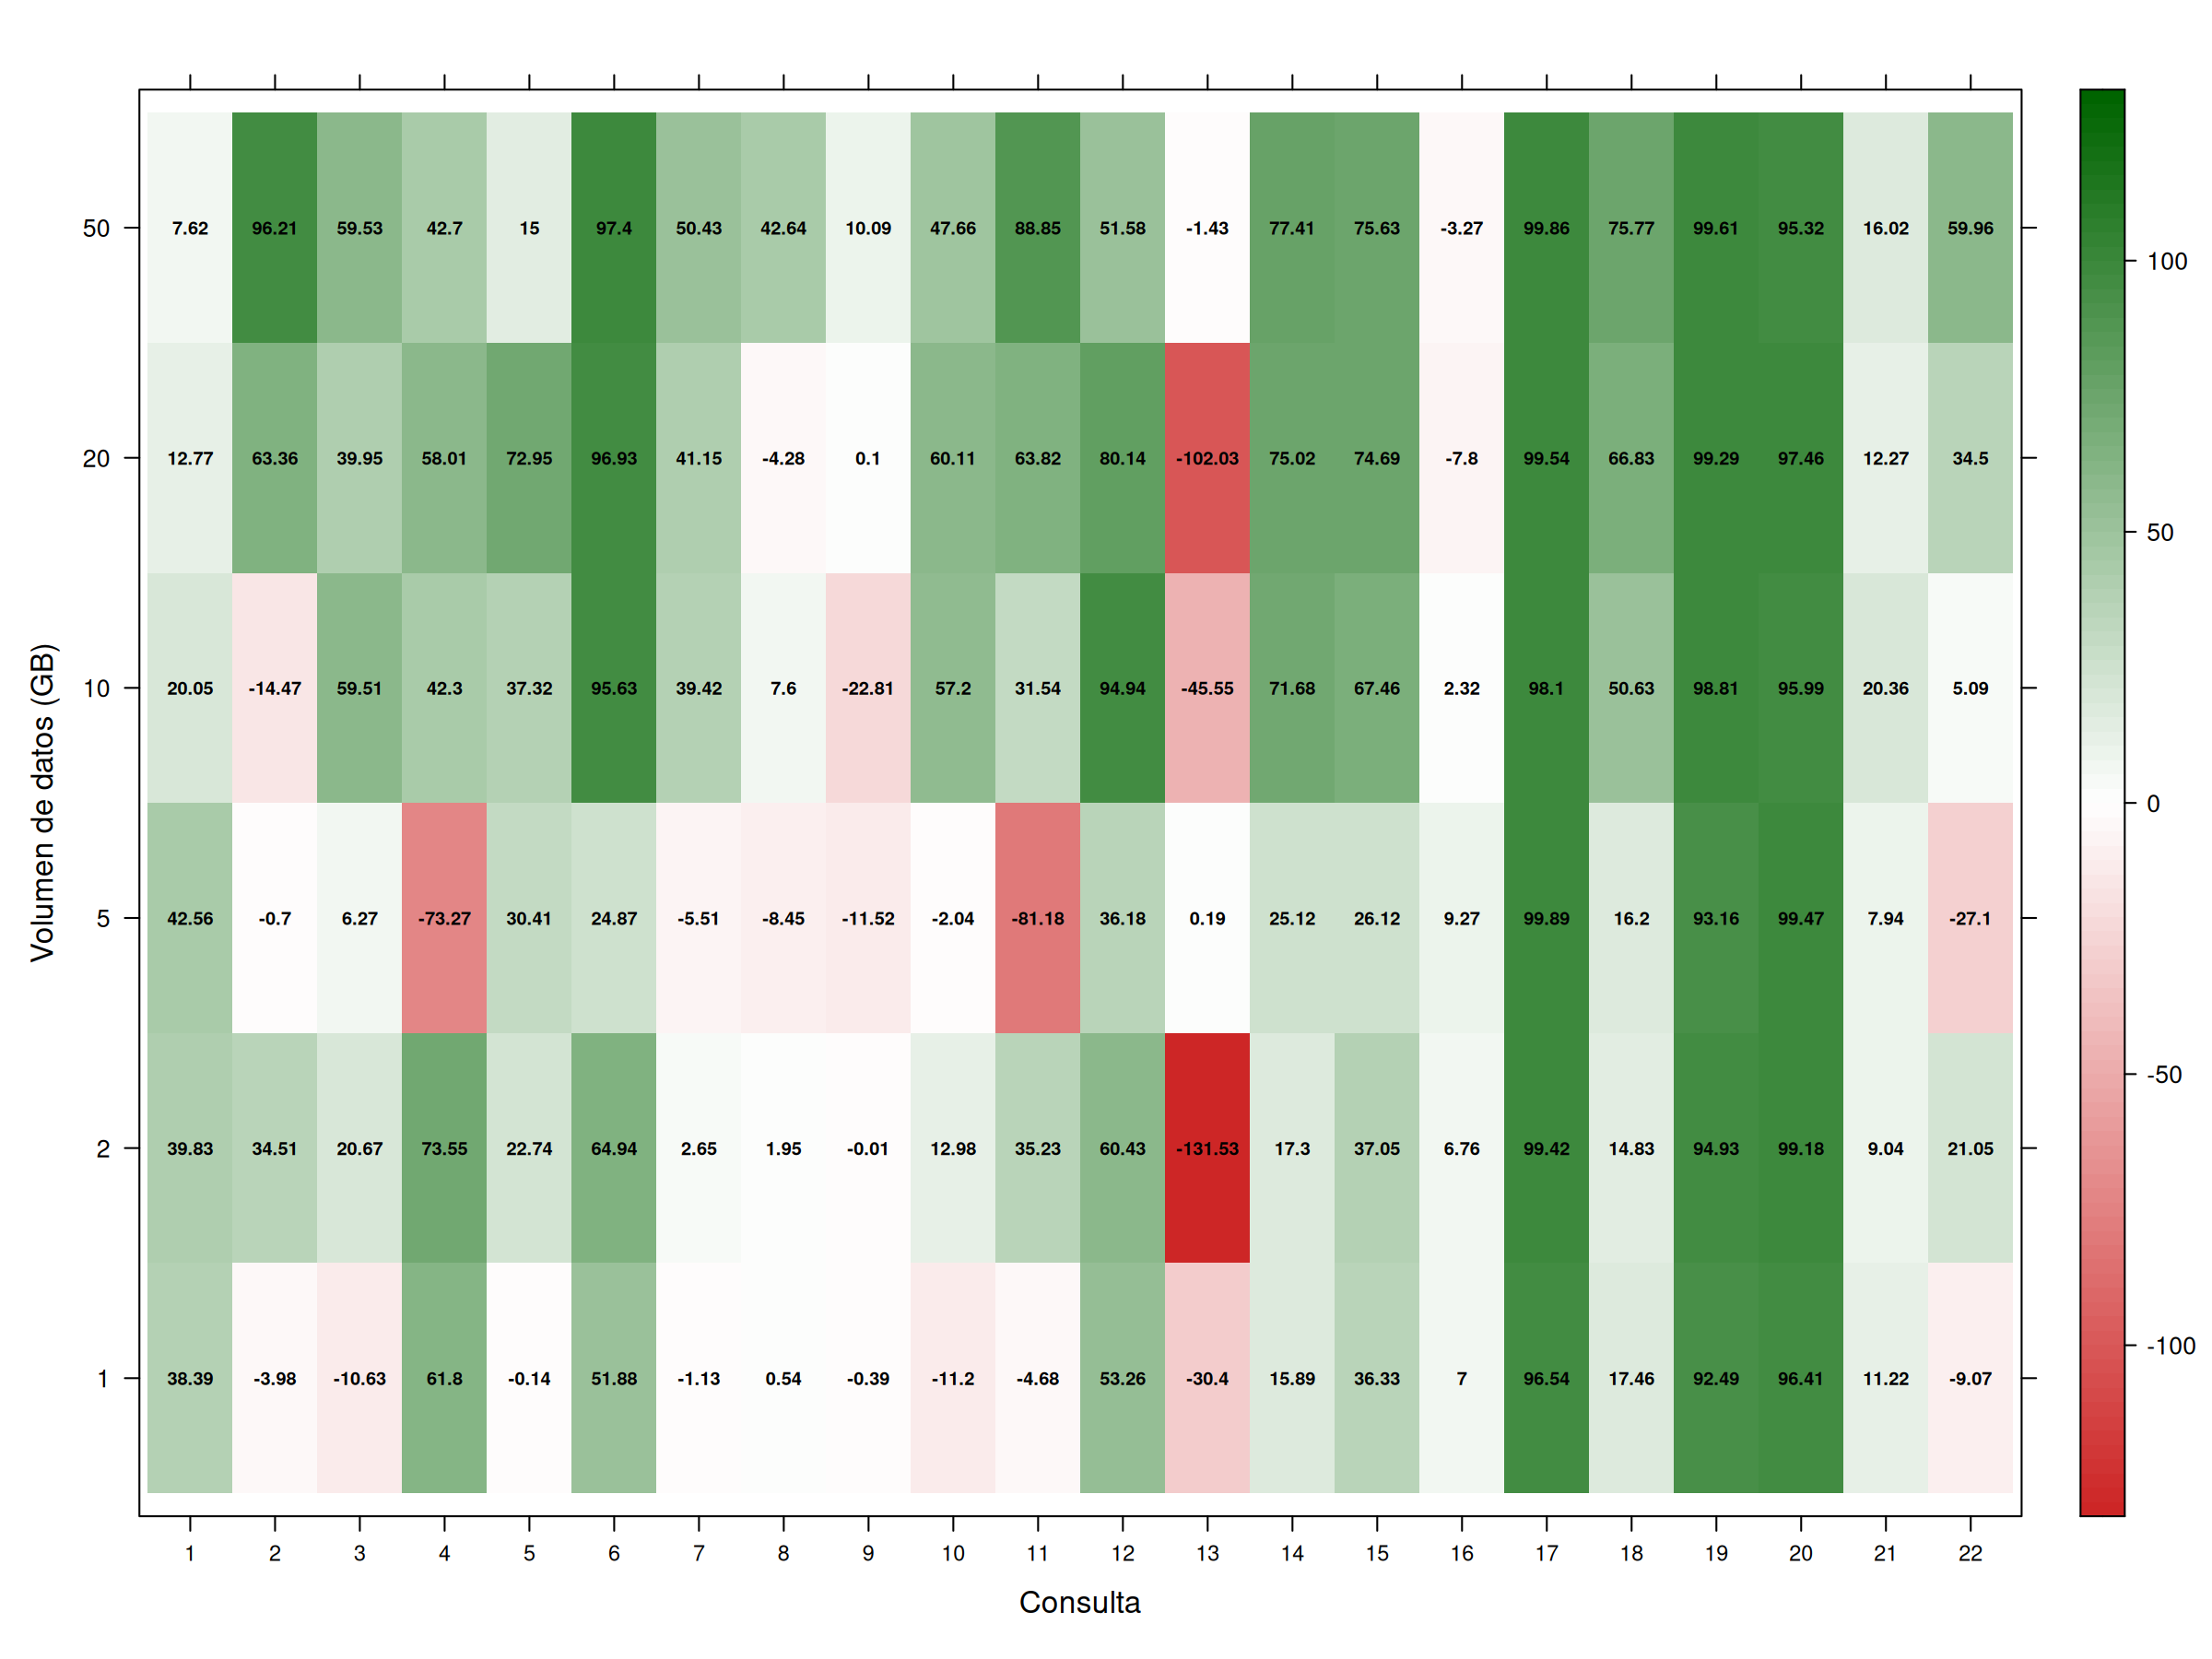
\includegraphics[width = \textwidth]{images/mejorasT.png}
          \caption{Mapa de calor de mejoras en rendimiento de las consultas}
          \label{fig:calorTiempo}
        \end{figure}

        El impacto neutro se debe a que el gestor, con base en sus estadísticas,
        decidió ignorar los índices propuestos y continuar con el plan en estado
        base. La mejora aislada a los dos gigabytes se explica porque los datos
        empiezan a desbordar la memoria caché y ese intercambio permite ver que
        la estrategia tiene éxito. Con diez gigabytes, el gestor cambió el plan
        de ejecución de lecturas secuenciales a ciclos anidados (\textit{nested
        loops}). Las lecturas secuenciales se optimizan en el manejo interno
        tanto del gestor como del sistema operativo de forma nativa
        \cite{graefe1993query}. Por su parte, los ciclos anidados rompen la
        secuencialidad y fuerzan los accesos aleatorios al disco, con los
        consecuentes \textit{buffer misses} (subsección
        \ref{sub:jerarquía_de_memoria_y_administración_del_buffer_pool}) y el
        respectivo incremento de la latencia. Sin embargo, cuando el volumen de
        datos se incrementa hasta los límites del almacenamiento (veinte y
        cincuenta gigabytes), incluso los accesos aleatorios se vuelven más
        eficientes, a pesar de los \textit{buffer misses} debido al descarte de
        páginas que vienen de los ciclos anidados.

        Para las consultas 3, 5, 7, 8, 9, 10 y 14, las cuales realizan
        particionamiento dinámico, se observa que, con un gigabyte, la
        estrategia de diseño no aporta mejoras e incluso llega a empeorar el
        desempeño (casos de la 3 y la 10). Esto ocurre porque el uso de índices
        introduce un \textit{overhead} que no supera la eficiencia de métodos
        más simples, como la lectura secuencial, cuando los datos residen
        íntegramente en la memoria caché. Con dos gigabytes, la estrategia
        comienza a ser efectiva para consultas ligeras (3, 5, 10 y 14). Sin
        embargo, en consultas más complejas como 7, 8 y 9, el beneficio sigue
        siendo opacado por el costo del particionamiento.

        Al alcanzar los cinco gigabytes, con la RAM cerca de su límite, sólo 5 y
        14 mantienen un crecimiento en su mejora, mientras que las demás sufren
        una degradación por la denominada tormenta de accesos aleatorios.
        Con diez gigabytes, a pesar de la necesidad de acceder al disco, las
        mejoras aumentan para casi todas las consultas, con excepción de la 9,
        cuyo volumen de lectura obligatorio y accesos aleatorios penalizan el
        tiempo de respuesta.

        Con veinte gigabytes, todas presentan mejoras salvo la 3 y la 8,
        probablemente debido a que el tamaño de los índices excede la memoria
        disponible. Finalmente, con cincuenta gigabytes y la capacidad física de
        los nodos al límite, los índices logran apoyar al sistema estresado. No
        obstante, en la 5 y la 9, la mejora es marginal debido a su baja
        selectividad y al excesivo tráfico de red generado. Cabe destacar que la
        14 fue la única consulta que exhibió una mejora monótona a través de
        todos los volúmenes de datos.

        Un segundo bloque de consultas, integrado por los casos 4, 6, 11, 12 y
        15, evidencia una vulnerabilidad crítica compartida a la escala de los
        cinco gigabytes. En este punto de inflexión, lo que coincide con la
        saturación del espacio de trabajo en la memoria RAM, todas ellas sufren
        una regresión en su desempeño. Este fenómeno colectivo responde a la 
        introducción de la tormenta de accesos aleatorios; a esta escala
        intermedia de datos, el costo de recuperar páginas dispersas mediante
        las nuevas estructuras de indexación resulta incapaz de superar la
        velocidad y eficiencia de las lecturas secuenciales que el gestor
        realizaba originalmente \cite{graefe1993query}.

        A pesar de este bache común, la evolución de estas consultas se bifurca
        al escalar el volumen de datos. Por un lado, las consultas 6, 11 y 15
        muestran un comportamiento homólogo posterior: tras el impacto adverso a
        los cinco gigabytes, inician un crecimiento sostenido a partir de los
        diez gigabytes. Una vez que la RAM se desborda por completo y el disco
        pasa a dominar los tiempos, la selectividad de la estrategia de diseño
        supera con creces las penalizaciones por acceso aleatorio del plan base.
        Por otro lado, la consulta 12 presenta una anomalía tardía a los veinte
        gigabytes, atribuible a que el tamaño crítico de sus índices específicos
        excede la capacidad de la memoria disponible para dicha operación, lo
        que replica el mecanismo de desborde analizado previamente en el bloque
        de consultas que realizan particionamiento dinámico.

        Las consultas 13, 16 y 22 representan los escenarios donde decisiones de
        diseño físico no alcanzaron la optimización esperada. En la 13, la
        introducción de una CTE no materializada provocó que el optimizador del
        gestor seleccionara rutas de ejecución subóptimas; de hecho, los
        rendimientos más bajos se registraron justamente al manifestarse las
        limitaciones físicas del hardware. En cuanto a consulta 16, centrar el
        diseño en el filtro \texttt{LIKE} con los comodines iniciales demostró
        no atacar el cuello de botella principal, el cual residía realmente en
        las tablas \texttt{partsupp} y \texttt{part} debido a su volumen
        significativamente mayor en comparación con \texttt{supplier}.

        Finalmente, respecto a la consulta 22, la estrategia exhibió un impacto
        intermitente. A la escala de un gigabyte, el rendimiento disminuyó
        debido a la superioridad de las lecturas secuenciales en caché frente a
        los accesos aleatorios del índice. A los diez gigabytes, este fenómeno
        de penalización se repitió: a pesar de que la tabla \texttt{customer}
        aún residía íntegramente en memoria, el costo computacional de los
        accesos aleatorios forzados por la consulta al índice superó el
        beneficio de la estructura física, lo que degradó el tiempo de respuesta
        frente a la lectura secuencial base.

        Las consultas 18 y 21 comparten tendencias similares, evidenciadas por
        mejoras inferiores al veinte por ciento en el escenario de un gigabyte,
        causadas por la velocidad de la memoria caché frente a hacer búsqueda
        indexada. A los dos gigabytes, su porcentaje de mejora disminuye por el
        incremento de accesos aleatorios. Sin embargo, a los cinco gigabytes
        ---con la memoria al límite de su capacidad--- el efecto del diseño se
        hace notar, a pesar de que el gestor seleccionó una ruta de ejecución
        poco favorable. Posteriormente, a los diez gigabytes, la mejora se
        recupera, aunque de forma moderada debido al beneficio intrínseco de las
        lecturas secuenciales para este perfil de consultas.

        A los veinte gigabytes, los comportamientos divergen: la 18 mejora
        mientras que la 21 no. La 18 progresa porque sus índices aún caben en
        RAM y su acceso aventaja a la lectura secuencial en disco. En contraste,
        la 21 se degrada porque, con ese volumen de datos y con la obligación de
        leer tres veces la tabla \texttt{lineitem}, el rendimiento colapsa por
        la densidad de accesos aleatorios al disco. No obstante, aunque ambas
        consultas elevan su mejora a los cincuenta gigabytes (con el hardware
        saturado), el beneficio en la consulta 18 supera en cinco veces al de la
        21.

        Finalmente, las consultas 17, 19 y 20 constituyen los escenarios donde
        la estrategia de diseño físico alcanzó su mayor impacto positivo,
        registrando optimizaciones cercanas al cien por ciento en todos los
        volúmenes estudiados. Este comportamiento excepcional y uniforme se
        fundamenta en la naturaleza específica de los mecanismos implementados.
        En los casos de la 17 y la 20, la incorporación de índices cobertores
        permitió al gestor resolver las demandas mediante lecturas exclusivas de
        índice, lo que elimina por completo la necesidad de acceder a las
        páginas de la tabla base. Por su parte, la consulta 19 capitalizó la
        co-locación física de las tablas \texttt{part} y \texttt{lineitem}
        (\texttt{lineitem\_by\_part}), lo que suprimió el costo de transferencia
        y reordenamiento de datos a través de la red durante las operaciones de
        unión (\texttt{JOIN}).

        De este modo, el beneficio de estas estructuras es tan determinante que
        vuelve al plan de ejecución inmune a las fluctuaciones de la memoria
        caché o el disco. Por lo tanto, más allá de las causas que gobiernan
        cada región del mapa de calor, es altamente probable que las sutiles
        diferencias en los porcentajes calculados para este grupo correspondan a
        la variabilidad propia del entorno experimental y no sean
        estadísticamente significativas.
      % subsection resumen_del_impacto_de_la_estrategia_de_diseño (end)

        En síntesis, el comportamiento de las consultas refleja que el escalado
        en el volumen de datos dicta una progresión ascendente en las demandas
        temporales del sistema. Ante este escenario, las estructuras de diseño
        físico implementadas logran mitigar este impacto de forma
        estadísticamente significativa en la mayor parte del espectro
        experimental, demostrando la viabilidad de la propuesta con la salvedad
        de las anomalías estructurales identificadas en los casos de las
        consultas 13, 16 y 22.

        No obstante, este beneficio en la velocidad de respuesta constituye solo
        una  dimensión del impacto arquitectónico; como señala la literatura
        científica especializada, la optimización del tiempo de ejecución no se
        traduce necesariamente en una reducción del consumo energético
        \cite{langtowards2009, langrethinking2011, niemanndoes2013}, fenómeno
        que se analiza en la sección siguiente.
    % section tiempos_de_ejecución (end)

    \section{Consumo energético neto} % (fold)
    \label{sec:consumo_energético_neto}
      Análogamente al análisis del tiempo de ejecución, se presenta en la tabla
      \ref{tab:neto} el consumo energético estimado para cada consulta con su
      media y desviación estándar. Asimismo, en las figuras \ref{fig:neto1} a
      \ref{fig:neto3}, se muestran los gráficos logarítmicos de consumo neto
      para las consultas en los diferentes volúmenes de datos.

      \subsection{Resumen de consumo neto} % (fold)
      \label{sub:resumen_de_consumo_neto}
        El consumo neto se calculó como la suma del consumo energético de cada
        nodo, mientras que la desviación estándar correspondiente se determinó
        mediante aplicación de la teoría de propagación de errores para
        cantidades aditivas \cite{skoog2013fundamentals} (ver ecuación
        (\ref{eq:propSuma})).

        \begin{equation}
          U_{neto} = \sum_{i = 1}^n U_i \Rightarrow
          \boxed{\sigma_{U_{neto}} = \sqrt{\sum_{i = 1}^n \sigma_{U_i}^2}}
          \label{eq:propSuma}
        \end{equation}

        Bajo un enfoque estrictamente teórico, la hipótesis que guía este
        análisis plantea que la estrategia de diseño físico disminuirá el
        consumo energético de las consultas y que, con el incremento del volumen
        de datos, se mantendrá la tendencia de mejora en términos relativos al
        escenario base sin optimizaciones.

        Sin embargo, al contrastar esta expectativa con los valores empíricos de
        la tabla \ref{tab:neto}, la primera observación destacable es que el
        consumo energético presenta un coeficiente de variación
        predominantemente superior o igual al treinta por ciento. Dicho umbral
        se considera como el rango de alta volatilidad \cite{jain1991art,
        montgomery2017design}. En efecto, esta condición se verifica en 134 de
        los 264 escenarios estudiados. Este fenómeno no responde a una falta de
        consistencia en las estrategias de diseño, sino a las limitaciones del
        muestreo para consultas con tiempos de ejecución menores a la unidad. Al
        ejecutarse las consultas en los escenarios con menor volumen de datos
        (uno y dos gigabytes) en menos de un segundo, la baja resolución
        temporal de las herramientas introdujo un ruido severo
        ---particularmente en el nodo coordinador debido a su rol de
        planificación---, el cual se propagó de forma incremental hacia la
        desviación del consumo neto final según la ecuación (\ref{eq:propSuma}).

        Al analizar la progresión de los datos en escenarios de mayor escala, se
        observa un incremento abrupto en los valores a partir del umbral de los
        diez gigabytes en consultas como la 4 y la 13. Es crucial destacar que
        este comportamiento no representa la presencia de valores atípicos, sino
        que refleja fielmente el quiebre operacional provocado por la transición
        hacia la lectura de disco. Al saturarse la memoria RAM disponible, el
        esfuerzo del hardware para solventar las operaciones de E/S en disco
        dispara la demanda energética en consonancia directa con el escalado del
        tiempo de ejecución.

        A su vez, el comportamiento de la consulta 16 en el escenario de veinte
        gigabytes merece una mención analítica particular, dado que registra un
        consumo masivo (18~971 J) con una desviación estándar extremadamente
        baja ($\pm 7$ J). La consistencia de esta varianza demuestra que no se
        trata de una anomalía estadística, sino de una decisión totalmente
        determinista del optimizador de consultas. Este fenómeno, conocido como
        un atrapamiento por costo del optimizador \cite{chaudhuri1998overview},
        ocurre por la combinación de una estrategia de indexación subóptima
        (índices sobre la tabla \textit{supplier} en lugar de \textit{part} o
        \textit{partsupp}) y la estructura interna de Q16, la cual emplea
        predicados \textit{LIKE} con comodines iniciales.

        A la escala de veinte gigabytes, los estimadores de costo del motor
        determinan erróneamente que el uso del índice disponible es ventajoso
        fuerzan un plan de ejecución degradado (como un bucle anidado o una
        lectura completa de índice) que se repite de forma idéntica en cada
        iteración. Paradójicamente, al escalar a cincuenta gigas, el volumen de
        datos supera el umbral de tolerancia del optimizador, lo que le obliga a
        abandonar dicho índice y conmutar hacia una lectura secuencial paralelo
        o un acoplamiento por hash (\textit{hash join}). Esta reestructuración
        del plan a gran escala resulta energéticamente más eficiente que el
        bucle catastrófico del escenario de veinte gigabytes, validando la
        consistencia interna del motor relacional.

        Por esta razón, formular aseveraciones deterministas sobre el impacto
        absoluto de la estrategia en el ahorro energético global a partir de
        estos valores promedios podría inducir a conclusiones sesgadas por el
        entorno experimental. En consecuencia, la evaluación de este
        comportamiento se aborda mediante un análisis de correlación no
        paramétrico (ver la sección \ref{sec:revision_estadistica}), el cual
        permite aislar la tendencia macro frente al ruido. Asimismo, se
        establece como trabajo futuro y necesidad metodológica explorar
        herramientas de alta frecuencia capaces de realizar mediciones
        energéticas precisas en ejecuciones sub-segundo.

      \subsection{Gráficos de barras: consumo contra volumen de datos} % (fold)
      \label{sub:gráficos_de_barras_consumo_contra_volumen_de_datos}
        En la figura \ref{fig:neto1}, se presentan dos diagramas de barras
        totalmente análogos a los diagramas de tiempo estudiados en la sección
        anterior. En tal sentido, se pueden distinguir de tres categorías de
        consultas: las que consumen poco (fracciones de joules), las de consumo
        moderado (menos de diez joules) y las de consumo alto (más de diez
        joules). El resultado de esta clasificación se muestra en la tabla
        \ref{tab:consultasPorConsumo}.

        Debido al volumen de datos, es esperado que la mayoría de las consultas
        registren consumos correspondientes a fracciones de joules, un
        comportamiento consistente con tiempos de ejecución inferiores a un
        segundo. Por lo tanto, el foco del análisis se centra en las consultas
        de consumo moderado y alto.

        \begin{landscape}
          \begin{table}
            \centering
            \begin{threeparttable}
              \caption{Consumo energético neto en joules sin diseño (SD) y con
              diseño (CD) físico\tnote{1}}
              \small
              \begin{tabular}{| l | l | l | l | l | l | l | l | l | l | l | l | l |}
                \hline \diagbox[width=4cm]{Consulta}{Carga (GB)}
                    &    1 (SD)    &    1  (CD)   &     2  (SD)    &     2  (CD)    &     5  (SD)     &     5  (CD)     &    10  (SD)    &    10  (CD)    &    20  (SD)    &    20  (CD)    &     50 (SD)     &     50 (CD)     \\ \hline
                Q1  & 0,2(5)       & 0,1(3)       & 1(1)\tnote{2}  & 3(5)           & 6(2)\tnote{2}   & 2(1)\tnote{2}   & 1,9(3)\tnote{3}& 8(2)\tnote{2}  & 4,5(4)\tnote{3}& 2,0(3)\tnote{3}& 1,18(5)\tnote{4}& 5,5(3)\tnote{3} \\ \hline
                Q2  & 0,027(2)     & 0,016(5)     & 0,04(1)        & 0,020(4)       & 0,05(2)         & 0,02(1)         & 0,02(2)        & 0,07(3)        & 1(1)           & 0,05(2)        & 5(1)\tnote{2}   & 27(4)           \\ \hline
                Q3  & 1(1)         & 1,2(8)       & 0,6(2)         & 1,1(9)         & 4(4)            & 3(2)            & 5(1)\tnote{2}  & 2(2)\tnote{2}  & 1,2(2)\tnote{3}& 1,0(2)\tnote{3}& 3,1(2)\tnote{3} & 3,1(3)\tnote{3} \\ \hline
                Q4  & 0,055(4)     & 0,019(5)     & 0,09(1)        & 0,037(8)       & 0,10(3)         & 0,1(1)          & 22(4)          & 4(2)           & 65(7)          & 20(6)          & 163(9)          & 1,2(1)\tnote{3} \\ \hline
                Q5  & 2(2)         & 1(1)         & 2(3)           & 1(1)           & 2(2)\tnote{2}   & 4(2)            & 90(2)\tnote{2} & 3(3)\tnote{2}  & 1,8(1)\tnote{3}& 1,8(3)\tnote{3}& 2,3(2)\tnote{3} & 1,9(2)\tnote{3} \\ \hline
                Q6  & 0,08(2)      & 0,018(4)     & 0,08(3)        & 0,020(5)       & 0,1(2)          & 0,03(2)         & 12(5)          & 0,03(2)        & 30(3)          & 0,02(1)        & 93(6)           & 0,03(6)         \\ \hline
                Q7  & 2(2)         & 2(1)         & 4(4)           & 2(1)           & 1(2)\tnote{2}   & 7(7)            & 37(9)          & 2(2)\tnote{2}  & 89(8)          & 6(3)\tnote{2}  & 2,3(3)\tnote{3} & 2,6(4)\tnote{3} \\ \hline
                Q8  & 10(7)        & 9(5)         & 2(1)\tnote{2}  & 3(2)\tnote{2}  & 6(3)\tnote{2}   & 7(4)\tnote{2}   & 1,9(4)\tnote{3}& 1,8(4)\tnote{3}& 4,0(4)\tnote{3}& 3,8(4)\tnote{3}& 9,7(6)\tnote{3} & 9,8(5)\tnote{3} \\ \hline
                Q9  & 3(2)\tnote{2}& 3(1)\tnote{2}& 7(4)\tnote{2}  & 8(4)\tnote{2}  & 2,4(4)\tnote{3} & 2,5(4)\tnote{3} & 4,8(4)\tnote{3}& 4,4(4)\tnote{3}& 9,8(5)\tnote{3}& 9,6(4)\tnote{3}& 2,24(9)\tnote{4}& 1,9(2)\tnote{4} \\ \hline
                Q10 & 1,2(8)       & 1,5(9)       & 1(1)           & 1,1(6)         & 4(2)            & 3(1)            & 3(1)\tnote{2}  & 9(2)           & 80(9)          & 3(1)\tnote{2}  & 2,7(2)\tnote{3} & 1,0(3)\tnote{3} \\ \hline
                Q11 & 0,029(5)     & 0,015(3)     & 0,029(7)       & 0,019(3)       & 0,05(3)         & 0,09(4)         & 0,1(3)         & 0,03(4)        & 0(1)           & 0,1(1)         & 3(1)\tnote{2}   & 0,08(1)         \\ \hline
                Q12 & 0,085(4)     & 0,022(5)     & 0,10(2)        & 0,08(1)        & 0,2(5)          & 0,02(3)         & 20(5)          & 0,02(2)        & 43(3)          & 6(6)           & 125(6)          & 9(1)\tnote{2}   \\ \hline
                Q13 & 0,037(4)     & 0,1(1)       & 0,04(2)        & 0,3(8)         & 0,06(2)         & 0,05(2)         & 3(9)           & 1(3)\tnote{5}  & 3(2)\tnote{2}  & 4(3)\tnote{2}  & 1,6(3)\tnote{3} & 1,3(6)\tnote{3} \\ \hline
                Q14 & 1,0(8)       & 1,2(7)       & 1,1(7)         & 9(8)           & 3(3)            & 1,1(7)          & 22(4)          & 4(2)           & 47(4)          & 9(4)           & 1,2(1)\tnote{3} & 2(1)\tnote{2}   \\ \hline
                Q15 & 0,07(1)      & 0,026(4)     & 0,4(9)         & 0(1)           & 9(8)            & 2(1)            & 5(2)\tnote{2}  & 8(2)           & 1,1(1)\tnote{3}& 4(2)\tnote{2}  & 3,0(3)\tnote{3} & 9(3)\tnote{2}   \\ \hline
                Q16 & 0,029(5)     & 0,026(4)     & 0,04(2)        & 0,04(2)        & 1,9(2)          & 2,53(7)         & 8(2)           & 7(1)           & 3(1)\tnote{2}  & 18 971(7)      & 1,3(3)\tnote{3} & 7(3)\tnote{2}   \\ \hline
                Q17 & 2(1)\tnote{2}& 0,013(7)     & 2,9(2)\tnote{3}& 2,9(2)\tnote{3}& 2,30(4)\tnote{4}& 0,012(6)        & 24(6)          & 0,012(5)       & 89(6)          & 0,03(2)        & 4,8(8)\tnote{3} & 0,04(1)         \\ \hline
                Q18 & 0,052(8)     & 0,05(1)      & 0,056(8)       & 0,05(2)        & 0,05(2)         & 0,01(1)         & 0,06(4)        & 0,03(3)        & 5(4)           & 0,04(6)        & 3(1)\tnote{2}   & 1(5)            \\ \hline
                Q19 & 0,8(6)       & 0,014(5)     & 2(2)           & 0,014(5)       & 0,05(2)         & 0,03(1)         & 39(7)          & 0,03(2)        & 76(7)          & 0,03(3)        & 2,2(1)\tnote{3} & 0,045(8)        \\ \hline
                Q20 & 5(2)e1       & 0,03(3)      & 4,6(2)\tnote{3}& 0,021(6)       & 10(6)           & 0,02(2)         & 24(7)          & 0,03(3)        & 6(1)\tnote{2}  & 0,03(5)        & 1,7(1)\tnote{3} & 4(7)            \\ \hline
                Q21 & 0,093(9)     & 0,10(2)      & 0,09(2)        & 0,10(2)        & 3,27(3)\tnote{4}& 1(3)            & 4(1)\tnote{2}  & 3(1)\tnote{2}  & 87(8)          & 68(6)          & 2,6(1)\tnote{3} & 174(7)          \\ \hline
                Q22 & 0,024(2)     & 0,022(3)     & 0,028(6)       & 0,030(6)       & 1(2)            & 0,1(1)          & 0,2(4)         & 1(2)           & 2(3)           & 1(3)           & 17(8)           & 18(9)           \\ \hline
              \end{tabular}
              \begin{tablenotes}
                \item[1] Los números entre paréntesis son la desviación estándar
                sobre la última cifra significativa.
                \item[2] medida $\times$ \num{e1}
                \item[3] medida $\times$ \num{e2}
                \item[4] medida $\times$ \num{e3}
                \item[5] medida $\times$ \num{e4}
              \end{tablenotes}
              \label{tab:neto}
            \end{threeparttable}
          \end{table}
        \end{landscape}

        % \begin{table}
        %   \centering
        %   \begin{threeparttable}
        %     \caption{Consumo energético (J) neto con diseño\tnote{1}}
        %     \footnotesize
        %     \begin{tabular}{| l | l | l | l | l | l | l |}
        %       \hline \diagbox[width=4cm]{Consulta}{Carga (GB)}
        %           &       1      &        2       &        5       &       10       &        20      &        50      \\ \hline
        %       Q1  & 0,1(3)       & 3(5)           & 2(1)\tnote{2}  & 8(2)\tnote{2}  & 2,0(3)\tnote{3}& 5,5(3)\tnote{3}\\ \hline
        %       Q2  & 0,016(5)     & 0,020(4)       & 0,02(1)        & 0,07(3)        & 0,05(2)        & 27(4)          \\ \hline
        %       Q3  & 1,2(8)       & 1,1(9)         & 3(2)           & 2(2)\tnote{2}  & 1,0(2)\tnote{3}& 3,1(3)\tnote{3}\\ \hline
        %       Q4  & 0,019(5)     & 0,037(8)       & 0,1(1)         & 4(2)           & 20(6)          & 1,2(1)\tnote{3}\\ \hline
        %       Q5  & 1(1)         & 1(1)           & 4(2)           & 3(3)\tnote{2}  & 1,8(3)\tnote{3}& 1,9(2)\tnote{3}\\ \hline
        %       Q6  & 0,018(4)     & 0,020(5)       & 0,03(2)        & 0,03(2)        & 0,02(1)        & 0,03(6)        \\ \hline
        %       Q7  & 2(1)         & 2(1)           & 7(7)           & 2(2)\tnote{2}  & 6(3)\tnote{2}  & 2,6(4)\tnote{3}\\ \hline
        %       Q8  & 9(5)         & 3(2)\tnote{2}  & 7(4)e1         & 1,8(4)\tnote{3}& 3,8(4)\tnote{3}& 9,8(5)\tnote{3}\\ \hline
        %       Q9  & 3(1)\tnote{2}& 8(4)\tnote{2}  & 2,5(4)\tnote{3}& 4,4(4)\tnote{3}& 9,6(4)\tnote{3}& 1,9(2)\tnote{4}\\ \hline
        %       Q10 & 1,5(9)       & 1,1(6)         & 3(1)           & 9(2)           & 3(1)\tnote{2}  & 1,0(3)\tnote{3}\\ \hline
        %       Q11 & 0,015(3)     & 0,019(3)       & 0,09(4)        & 0,03(4)        & 0,1(1)         & 0,08(1)        \\ \hline
        %       Q12 & 0,022(5)     & 0,08(1)        & 0,02(3)        & 0,02(2)        & 6(6)           & 9(1)\tnote{2}  \\ \hline
        %       Q13 & 0,1(1)       & 0,3(8)         & 0,05(2)        & 1(3)\tnote{5}  & 4(3)\tnote{2}  & 1,3(6)\tnote{3}\\ \hline
        %       Q14 & 1,2(7)       & 9(8)           & 1,1(7)         & 4(2)           & 9(4)           & 2(1)\tnote{2}  \\ \hline
        %       Q15 & 0,026(4)     & 0(1)           & 2(1)           & 8(2)           & 4(2)\tnote{2}  & 9(3)\tnote{2}  \\ \hline
        %       Q16 & 0,026(4)     & 0,04(2)        & 2,53(7)        & 7(1)           & 18 971(7)      & 7(3)\tnote{2}  \\ \hline
        %       Q17 & 0,013(7)     & 2,9(2)\tnote{3}& 0,012(6)       & 0,012(5)       & 0,03(2)        & 0,04(1)        \\ \hline
        %       Q18 & 0,05(1)      & 0,05(2)        & 0,01(1)        & 0,03(3)        & 0,04(6)        & 1(5)           \\ \hline
        %       Q19 & 0,014(5)     & 0,014(5)       & 0,03(1)        & 0,03(2)        & 0,03(3)        & 0,045(8)       \\ \hline
        %       Q20 & 0,03(3)      & 0,021(6)       & 0,02(2)        & 0,03(3)        & 0,03(5)        & 4(7)           \\ \hline
        %       Q21 & 0,10(2)      & 0,10(2)        & 1(3)           & 3(1)\tnote{2}  & 68(6)          & 174(7)         \\ \hline
        %       Q22 & 0,022(3)     & 0,030(6)       & 0,1(1)         & 1(2)           & 1(3)           & 18(9)          \\ \hline
        %     \end{tabular}
        %     \begin{tablenotes}
        %       \item[1] Los números entre paréntesis son la desviación estándar
        %       sobre la última cifra significativa.
        %     \end{tablenotes}
        %     \label{tab:netoCD}
        %   \end{threeparttable}
        % \end{table}
      % subsection resumen_de_consumo_neto (end)

        \begin{figure}[H]
          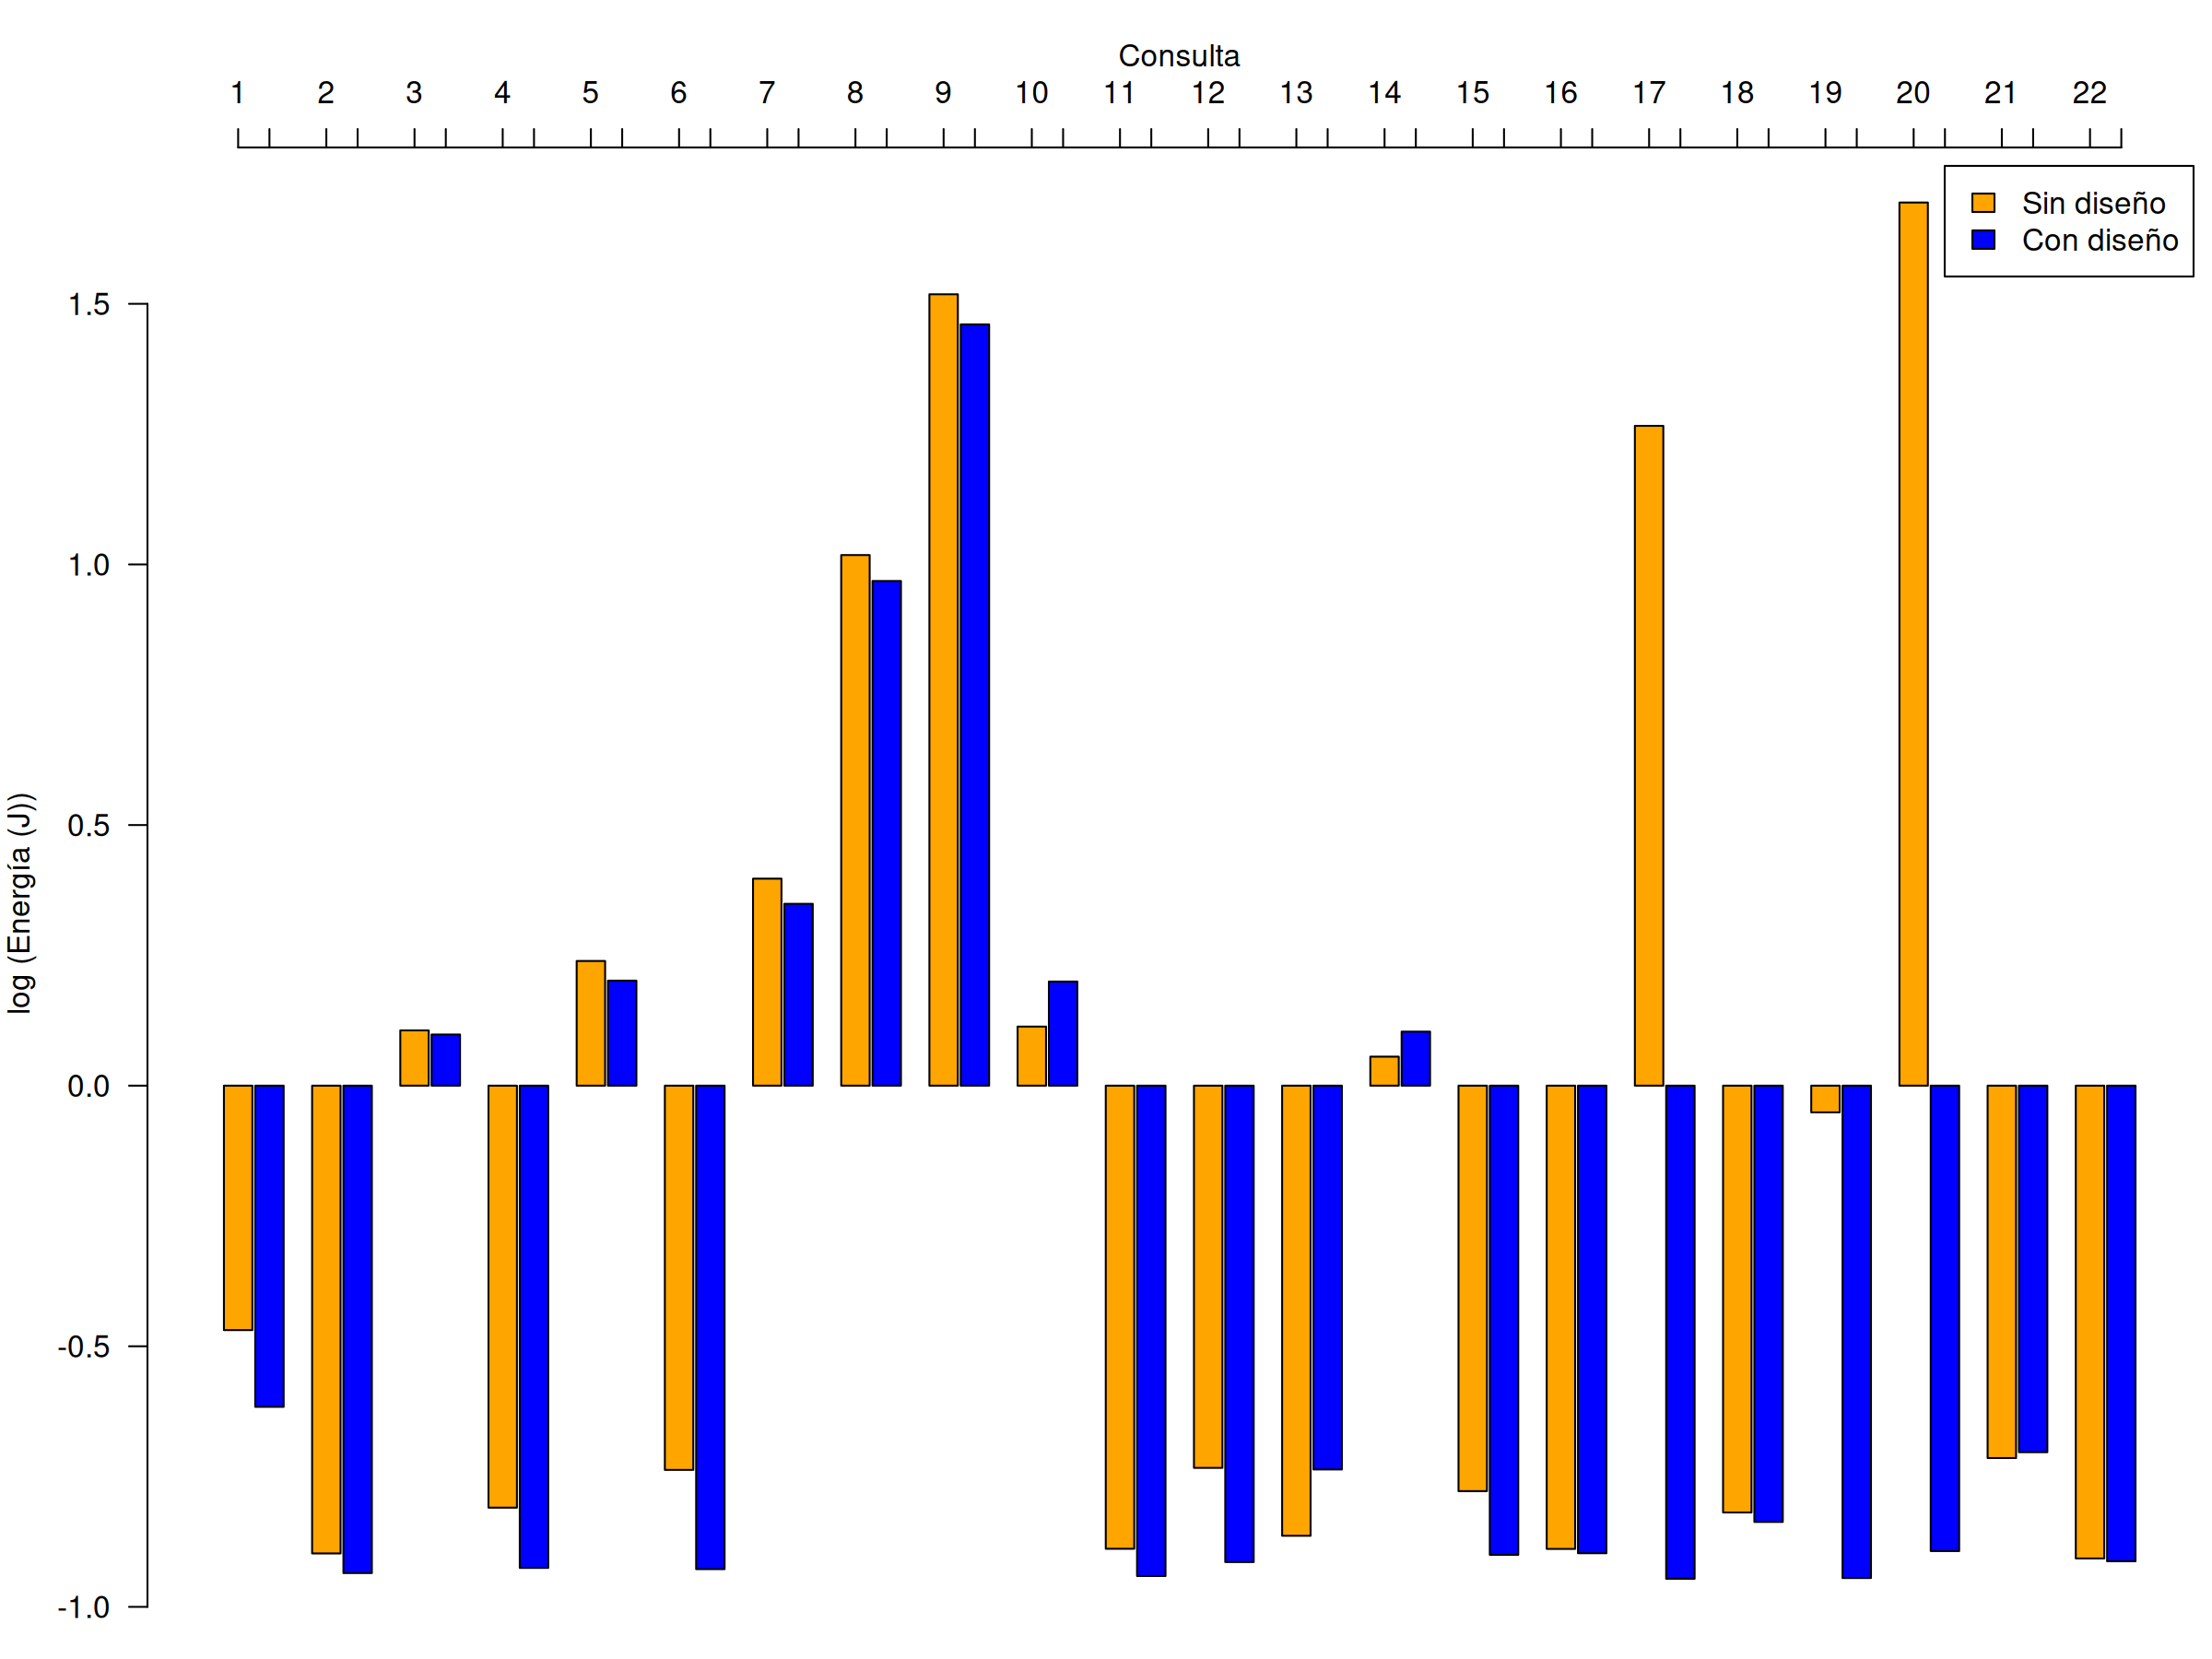
\includegraphics[width = 0.5\textwidth]{images/Neto-1G.png}
          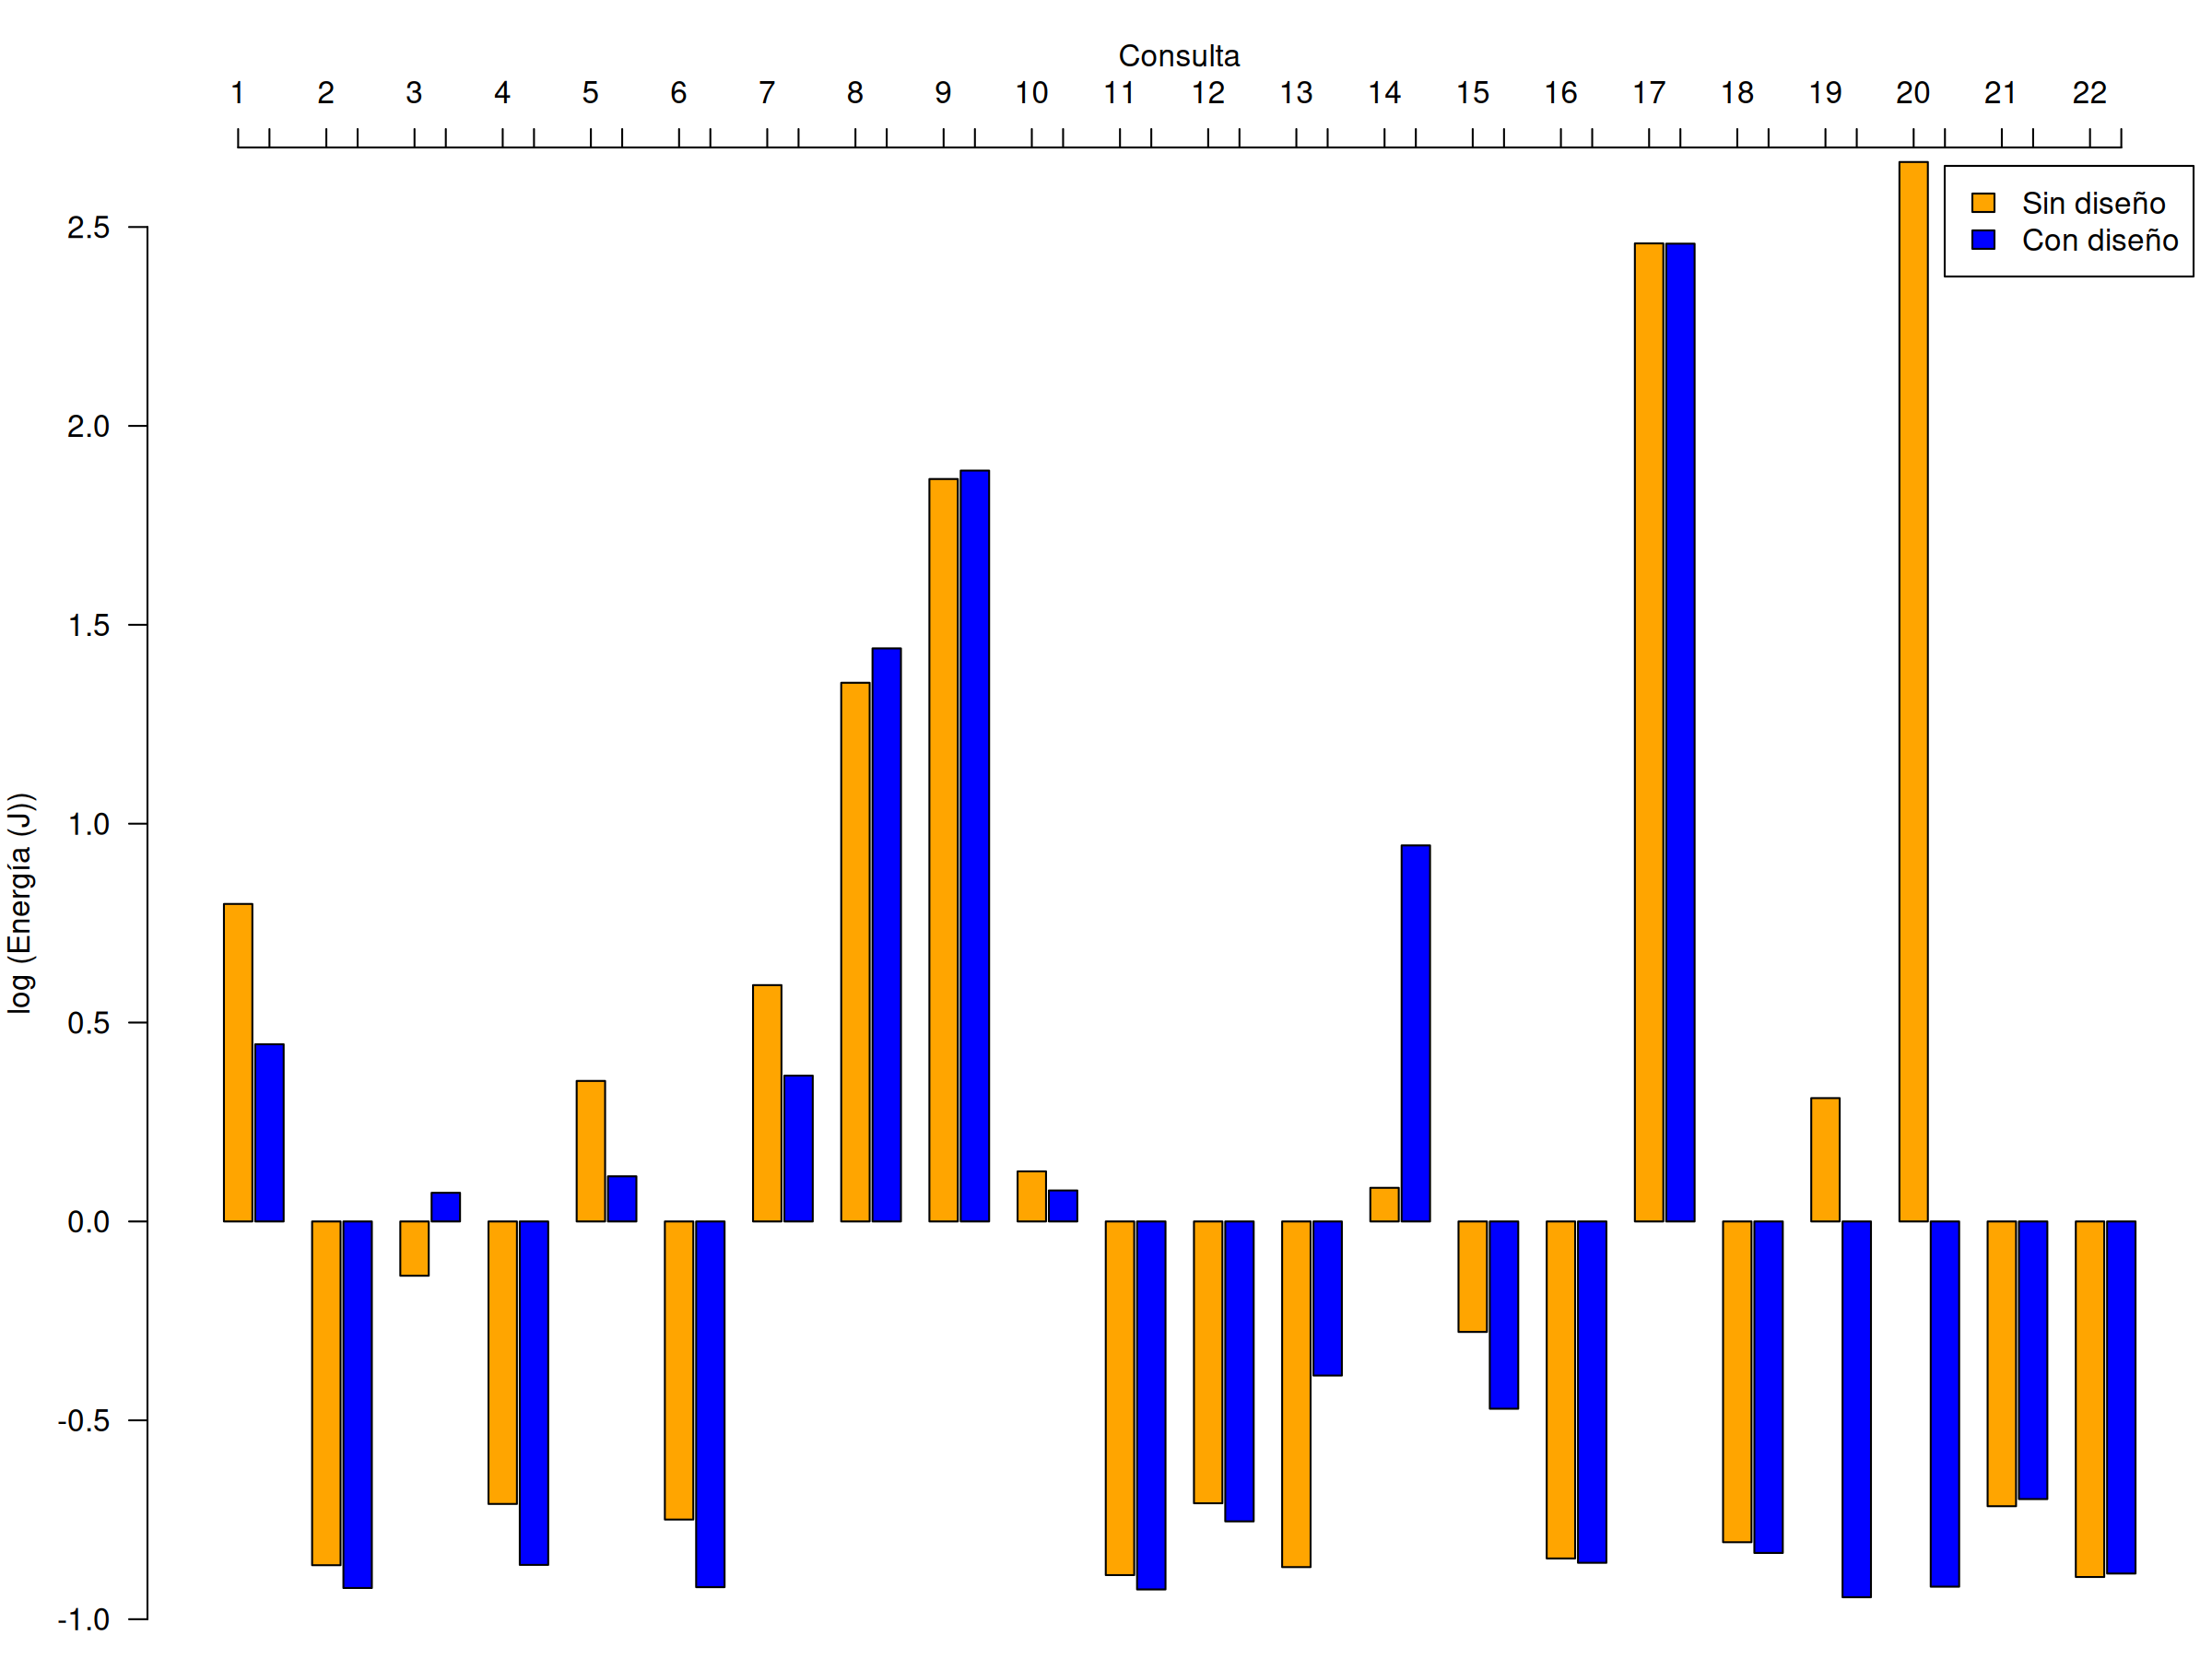
\includegraphics[width = 0.5\textwidth]{images/Neto-2G.png}
          \caption{Consumo neto por consulta 1 GB (izquierda) y 2 GB (derecha)}
          \label{fig:neto1}
        \end{figure}

        El gasto energético de la consulta 3 está condicionado por el costo del
        particionamiento dinámico al realizar la unión de tablas no co-locadas.
        La estrategia de diseño físico implementada para esta operación
        consistió en la creación de índices, pero debido al particionamiento
        dinámico, el plan de ejecución global no reporta las tareas hechas por
        los nodos trabajadores. A pesar de esta limitación de observabilidad en
        el nodo coordinador, la disminución registrada en el tiempo de ejecución
        permite inferir que los optimizadores locales de los nodos trabajadores
        utilizaron efectivamente las estructuras indexadas
        \cite{citus_query_processing, citus_performance_tuning}.

        Este uso se evidencia de forma analítica al contrastar las escalas de 
        uno y dos gigabytes (ver figura \ref{fig:neto1}). Mientras que a un
        gigabyte se registra una ligera atenuación energética, el escenario de
        dos gigabytes con estrategia de diseño exhibe un incremento en el
        consumo respecto al caso base. Este comportamiento constituye el
        indicador físico de la activación del índice: al duplicarse el volumen,
        el patrón de acceso aleatorio inherente a la búsqueda indexada desborda
        las líneas de la memoria caché, provocando un incremento severo en los
        fallos de búfer (\textit{buffer misses}) en comparación con la
        predictibilidad y eficiencia del pre-procesamiento lineal de una lectura
        secuencial. Por lo tanto, el aumento energético no deviene de la
        inactividad de la estrategia, sino del costo de hardware asociado al
        acceso no contiguo a los datos en esta escala volumétrica. Por el
        contrario, en las escalas de cinco y diez gigabytes (ver figura
        \ref{fig:neto2}) se alcanza el punto óptimo de la estrategia, donde se
        registra una disminución significativadel consumo. En este rango, el
        volumen de datos ya justifica la búsqueda indexada, puesto que la
        reducción drástica en el total de operaciones de E/S compensa el costo
        de los accesos aleatorios a disco frente a una lectura secuencial
        masiva.

        Finalmente, al escalar a los escenarios de veinte y cincuenta gigabytes
        (ver figura \ref{fig:neto3}), la consulta deja de experimentar
        variaciones significativas tras la implementación de la estrategia de
        diseño físico. Este estancamiento responde al fenómeno de desbordamiento
        en disco durante la fase de particionamiento dinámico: al saturarse la
        memoria intermedia de los trabajadores, el sistema se ve obligado a
        realizar operaciones masivas de escritura y lectura de archivos
        temporales en disco, un cuello de botella de E/S de alta demanda
        energética que termina por neutralizar cualquier beneficio teórico
        aportado por la indexación local.

        Por su parte, la consulta 4 opera sobre la segunda tabla de mayor
        volumen, \texttt{orders}, e incluye una consulta anidada correlacionada
        con \texttt{lineitem}. Al tratarse de tablas co-locadas, el intercambio
        de datos a través de la red es nulo, lo que se traduce en un perfil de
        consumo altamente eficiente que, en las escalas de uno y dos gigabytes,
        se mantiene por debajo de los diez joules.

        \begin{figure}[H]
          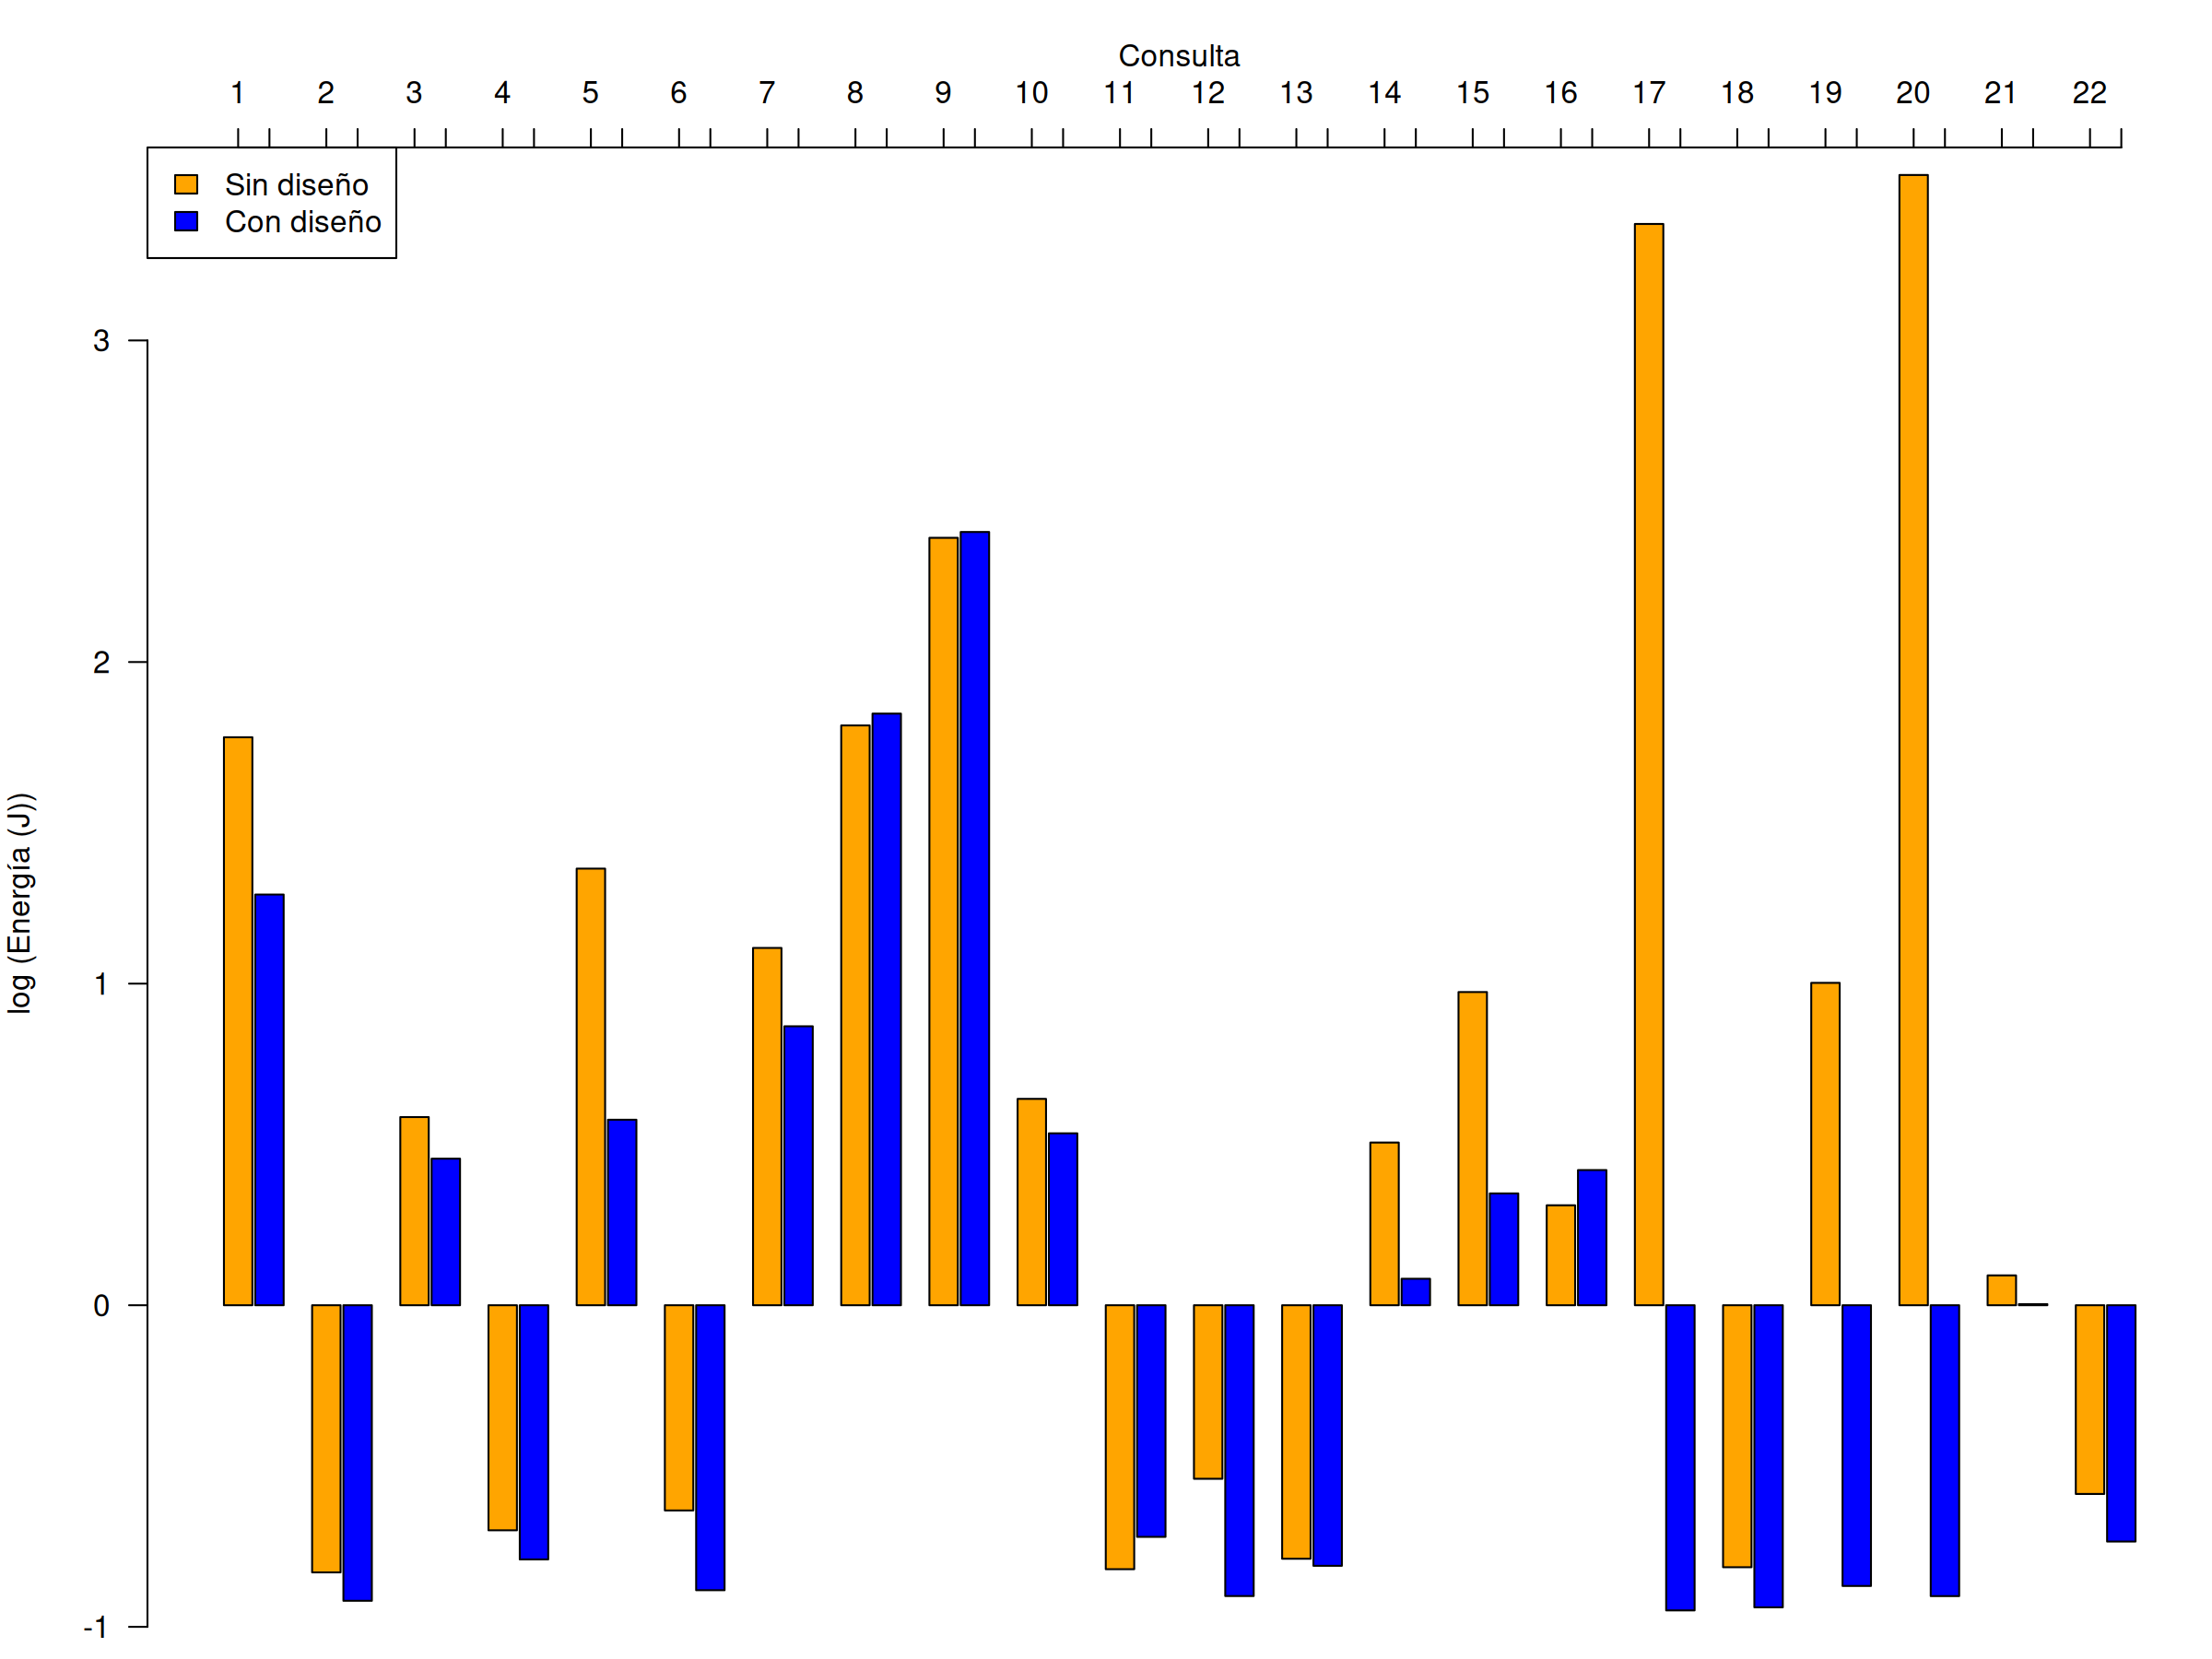
\includegraphics[width = 0.5\textwidth]{images/Neto-5G.png}
          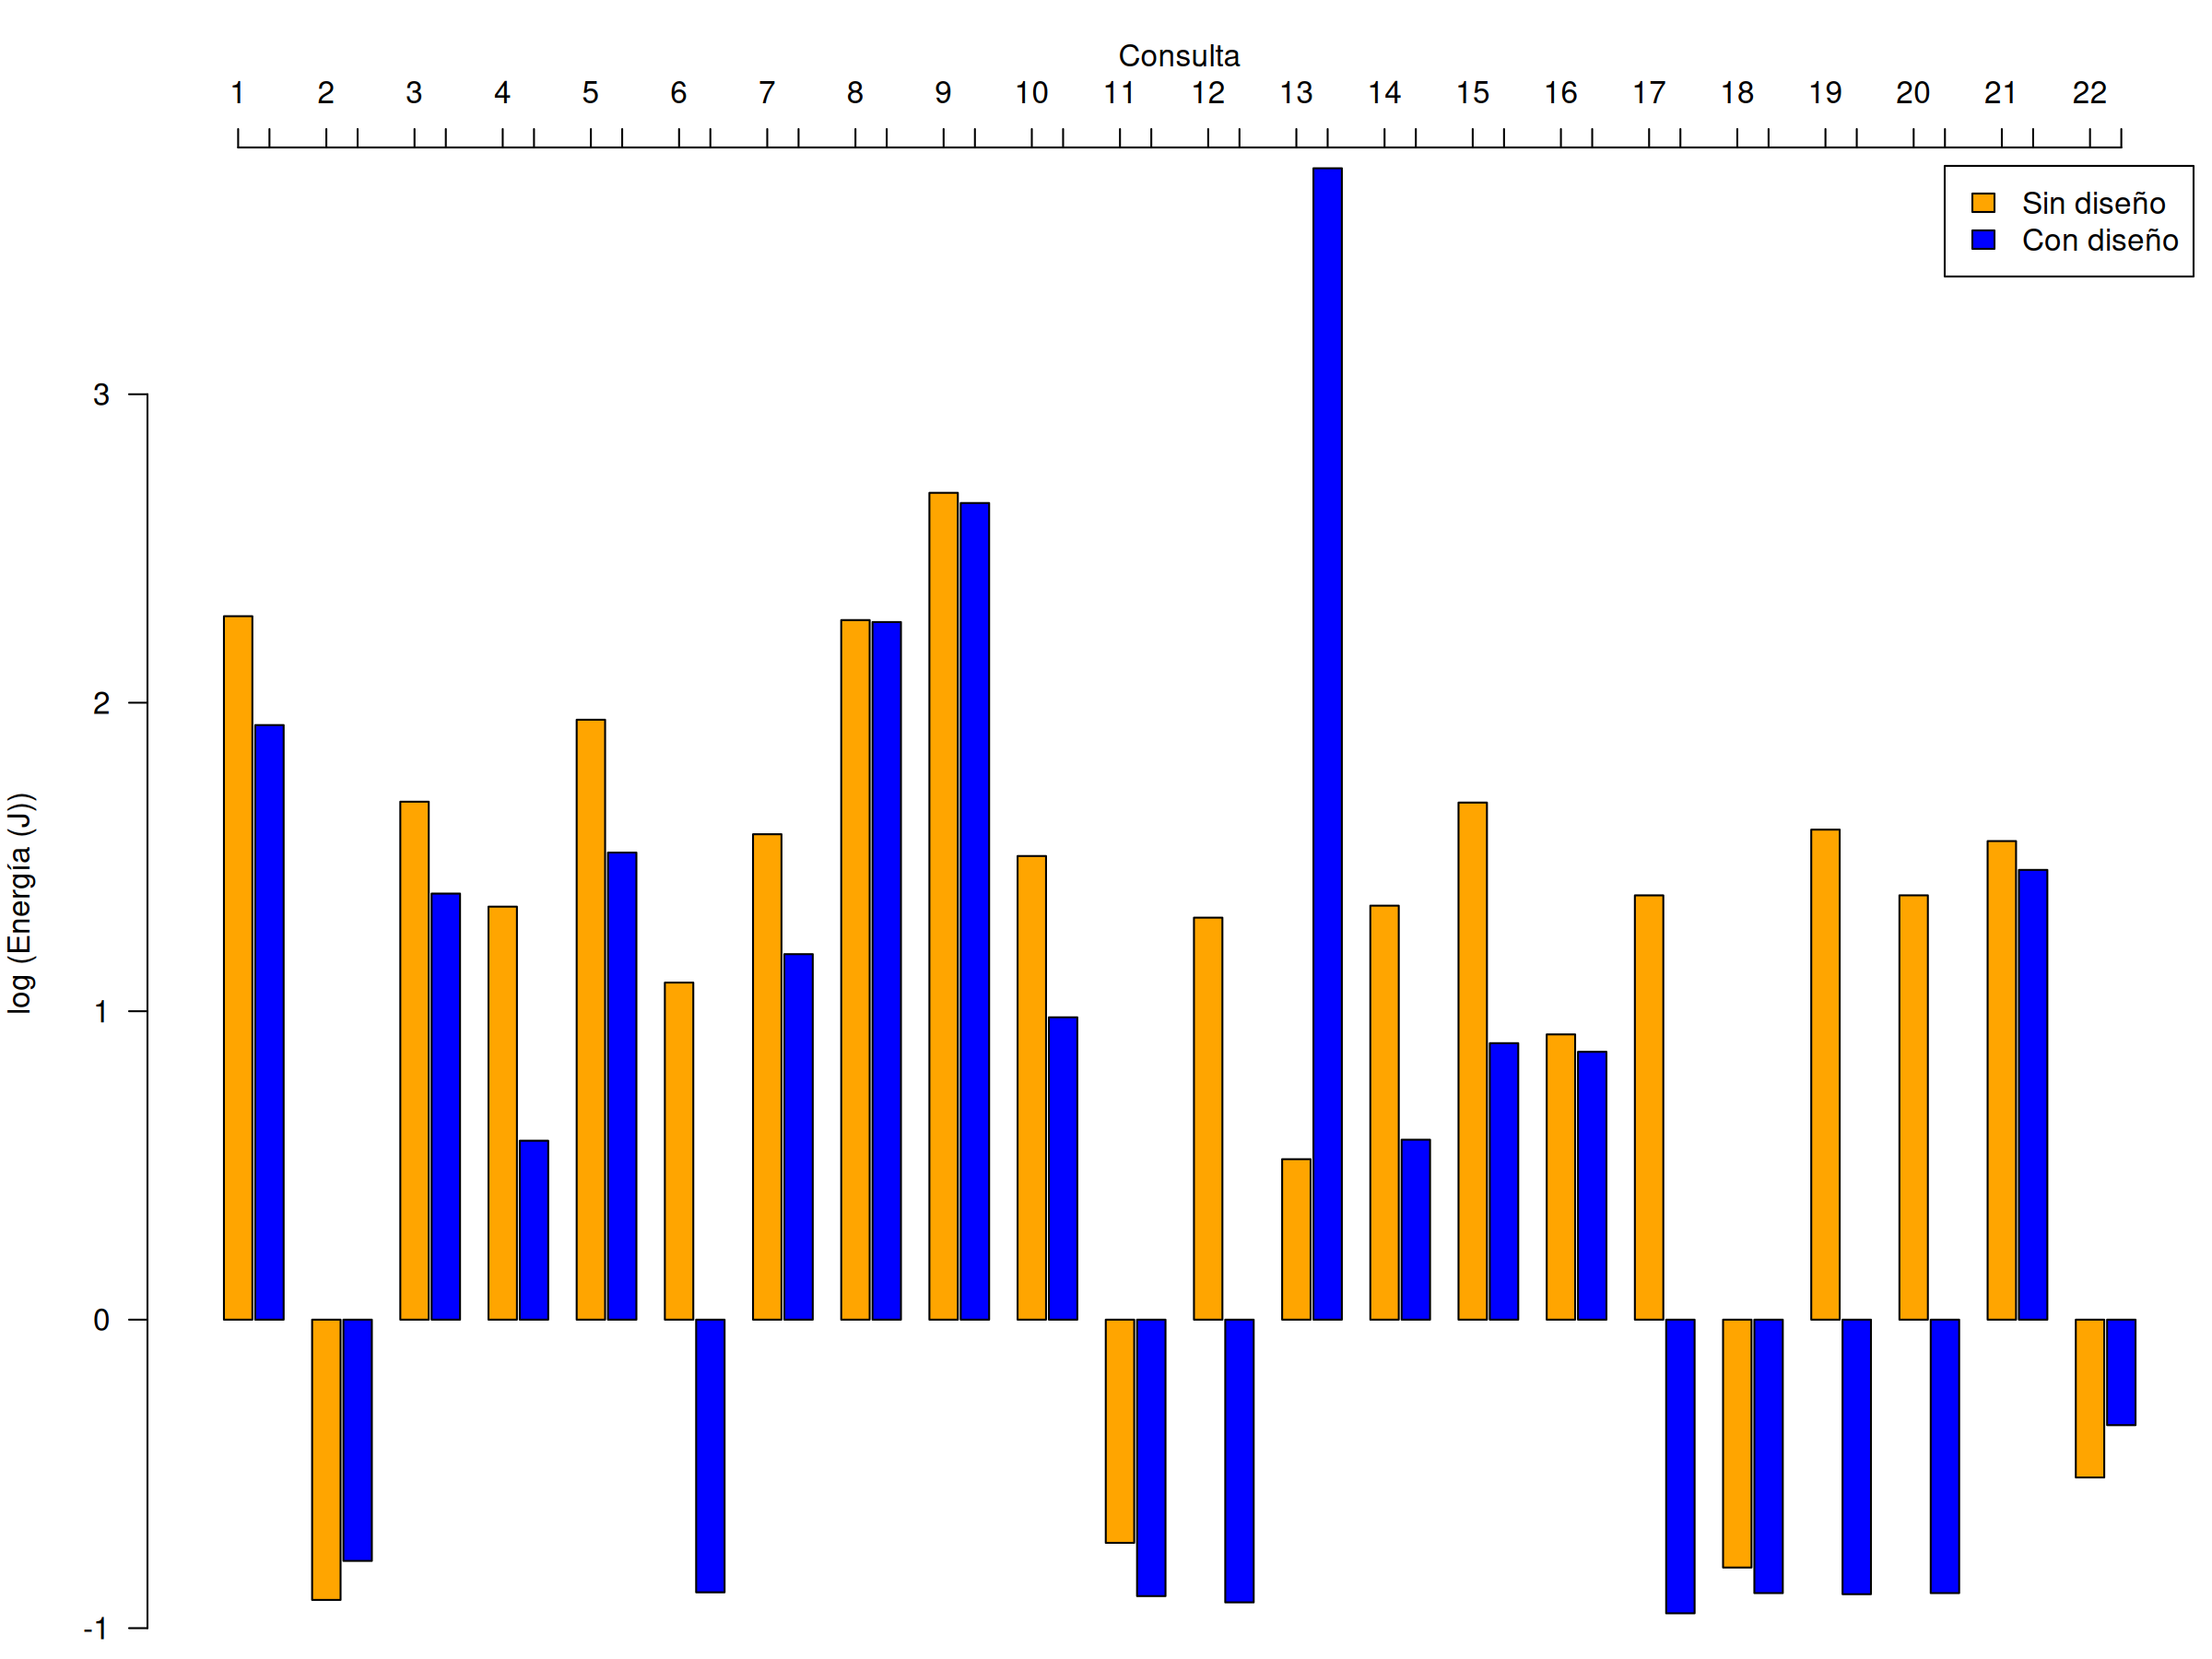
\includegraphics[width = 0.5\textwidth]{images/Neto-10G.png}
          \caption{Consumo neto por consulta 5 GB (izquierda) y 10 GB (derecha)}
          \label{fig:neto2}
        \end{figure}

        \begin{figure}[H]
          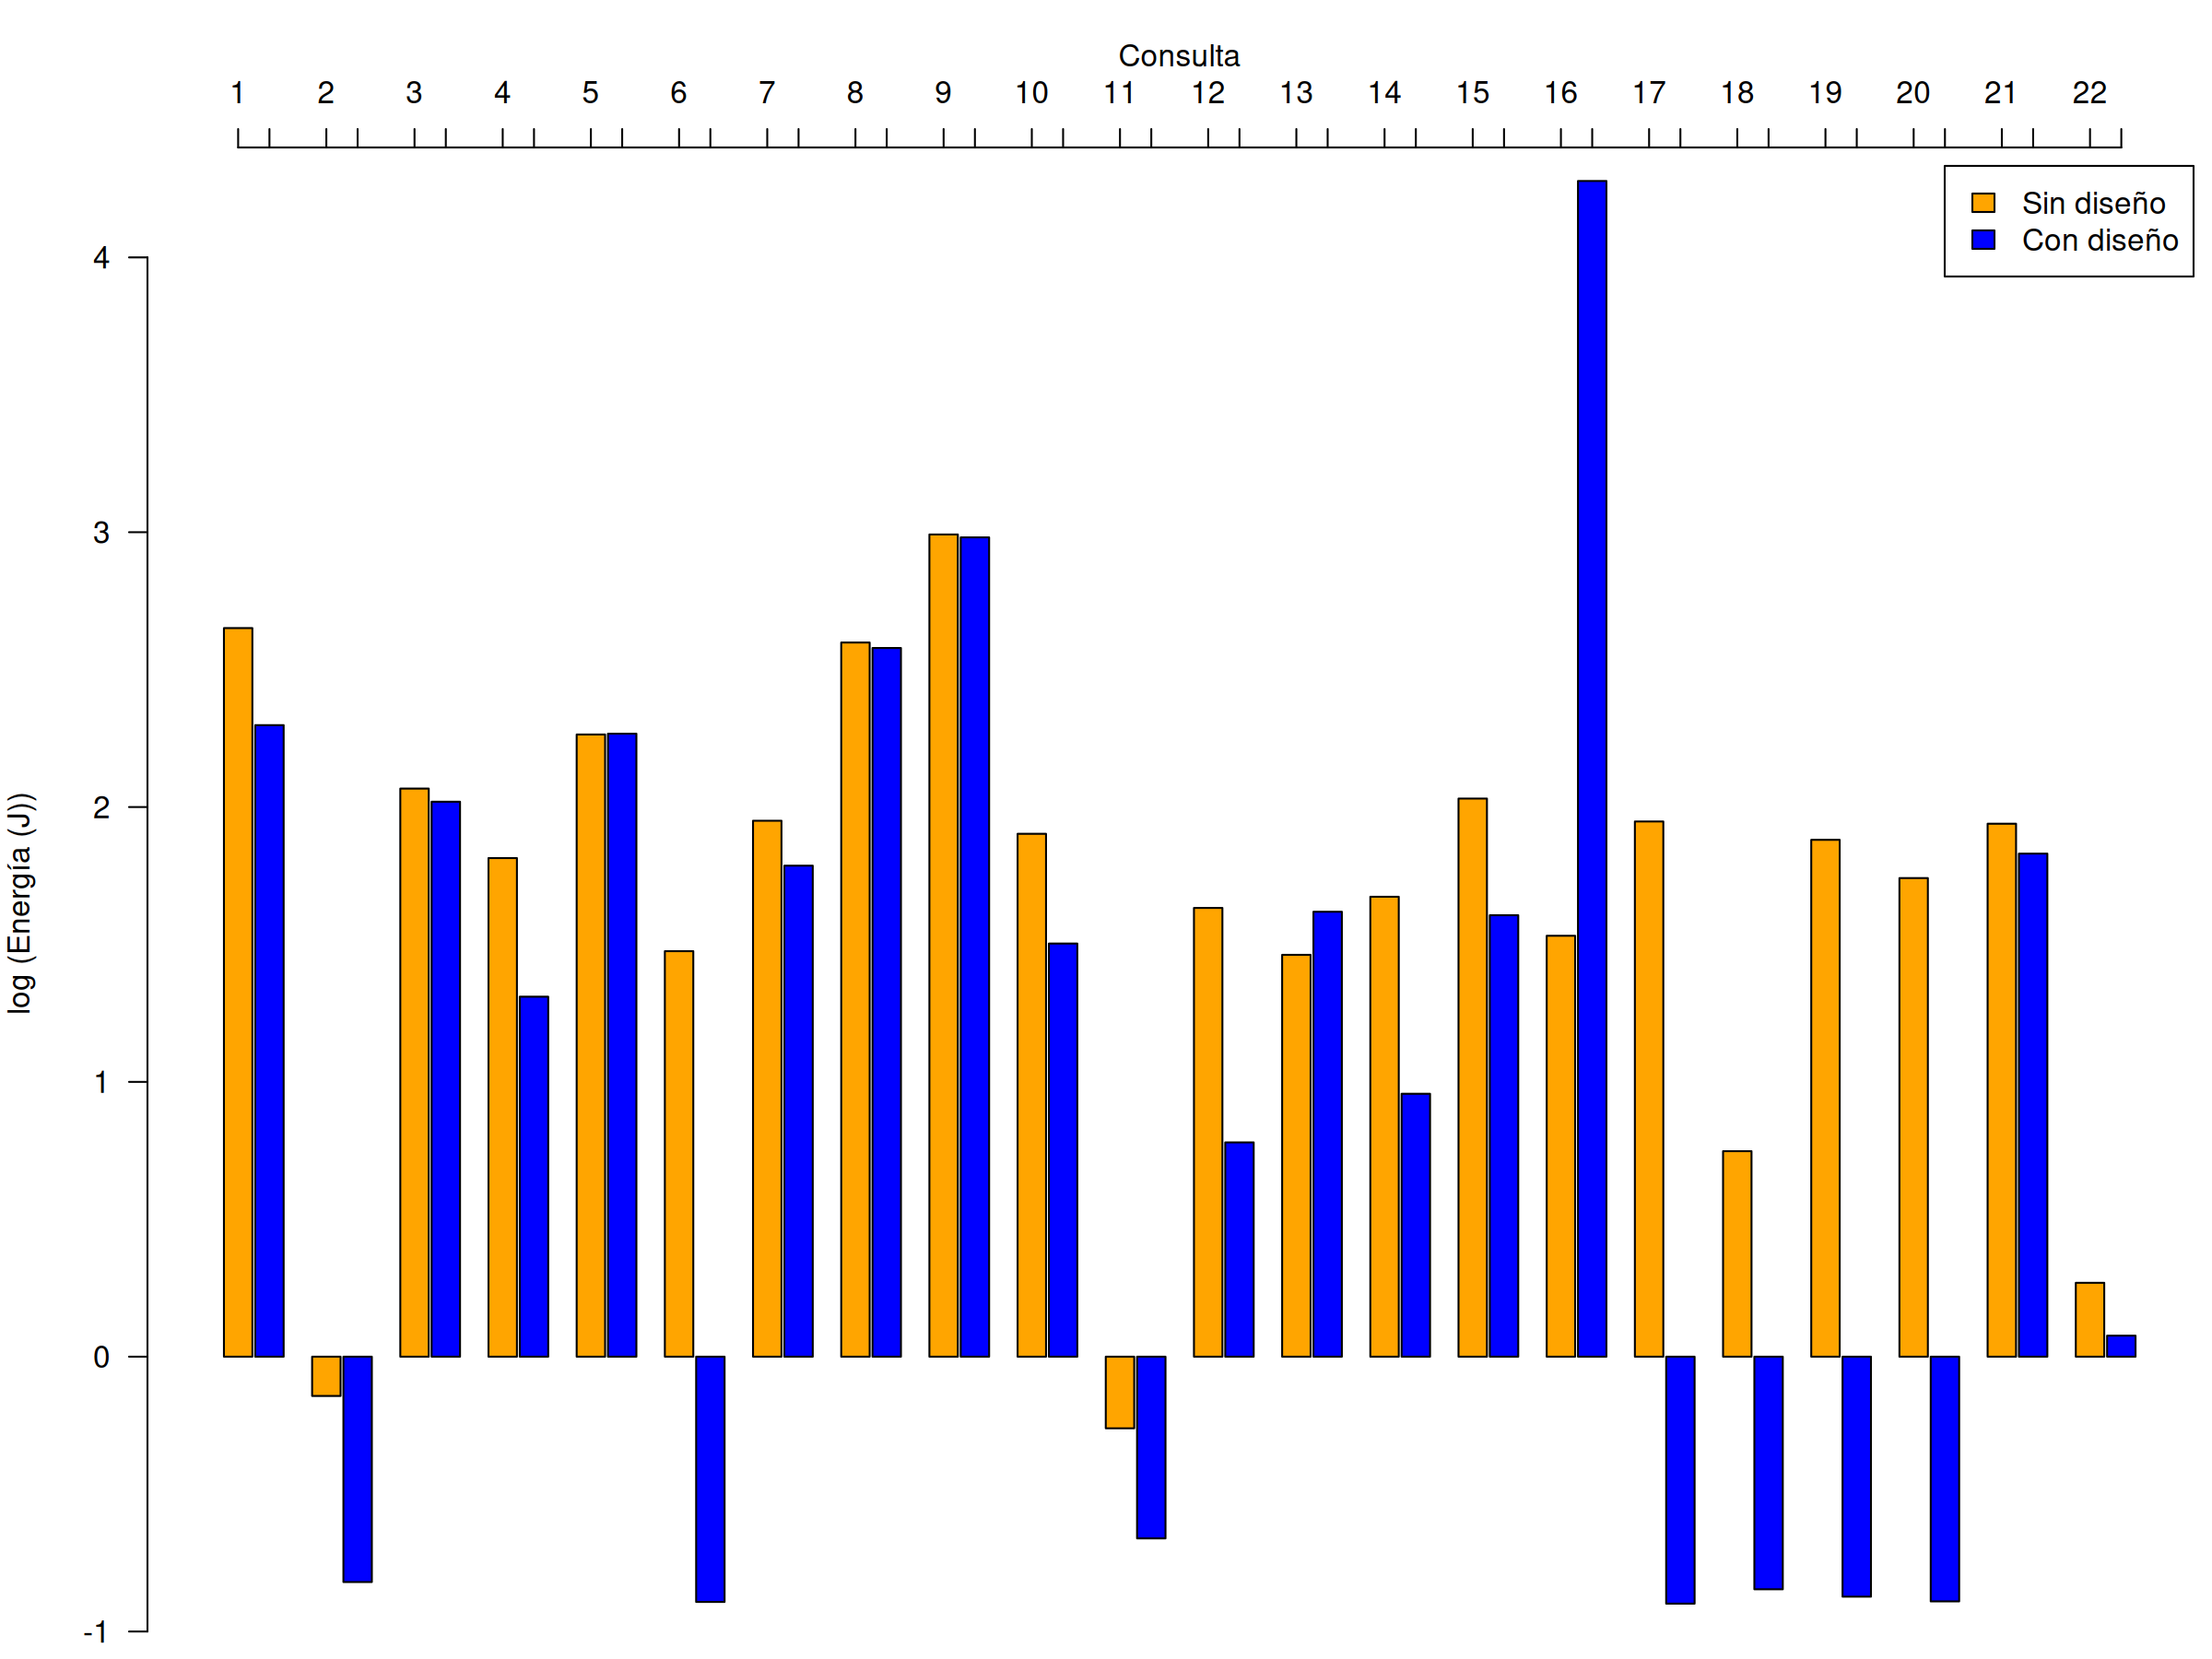
\includegraphics[width = 0.5\textwidth]{images/Neto-20G.png}
          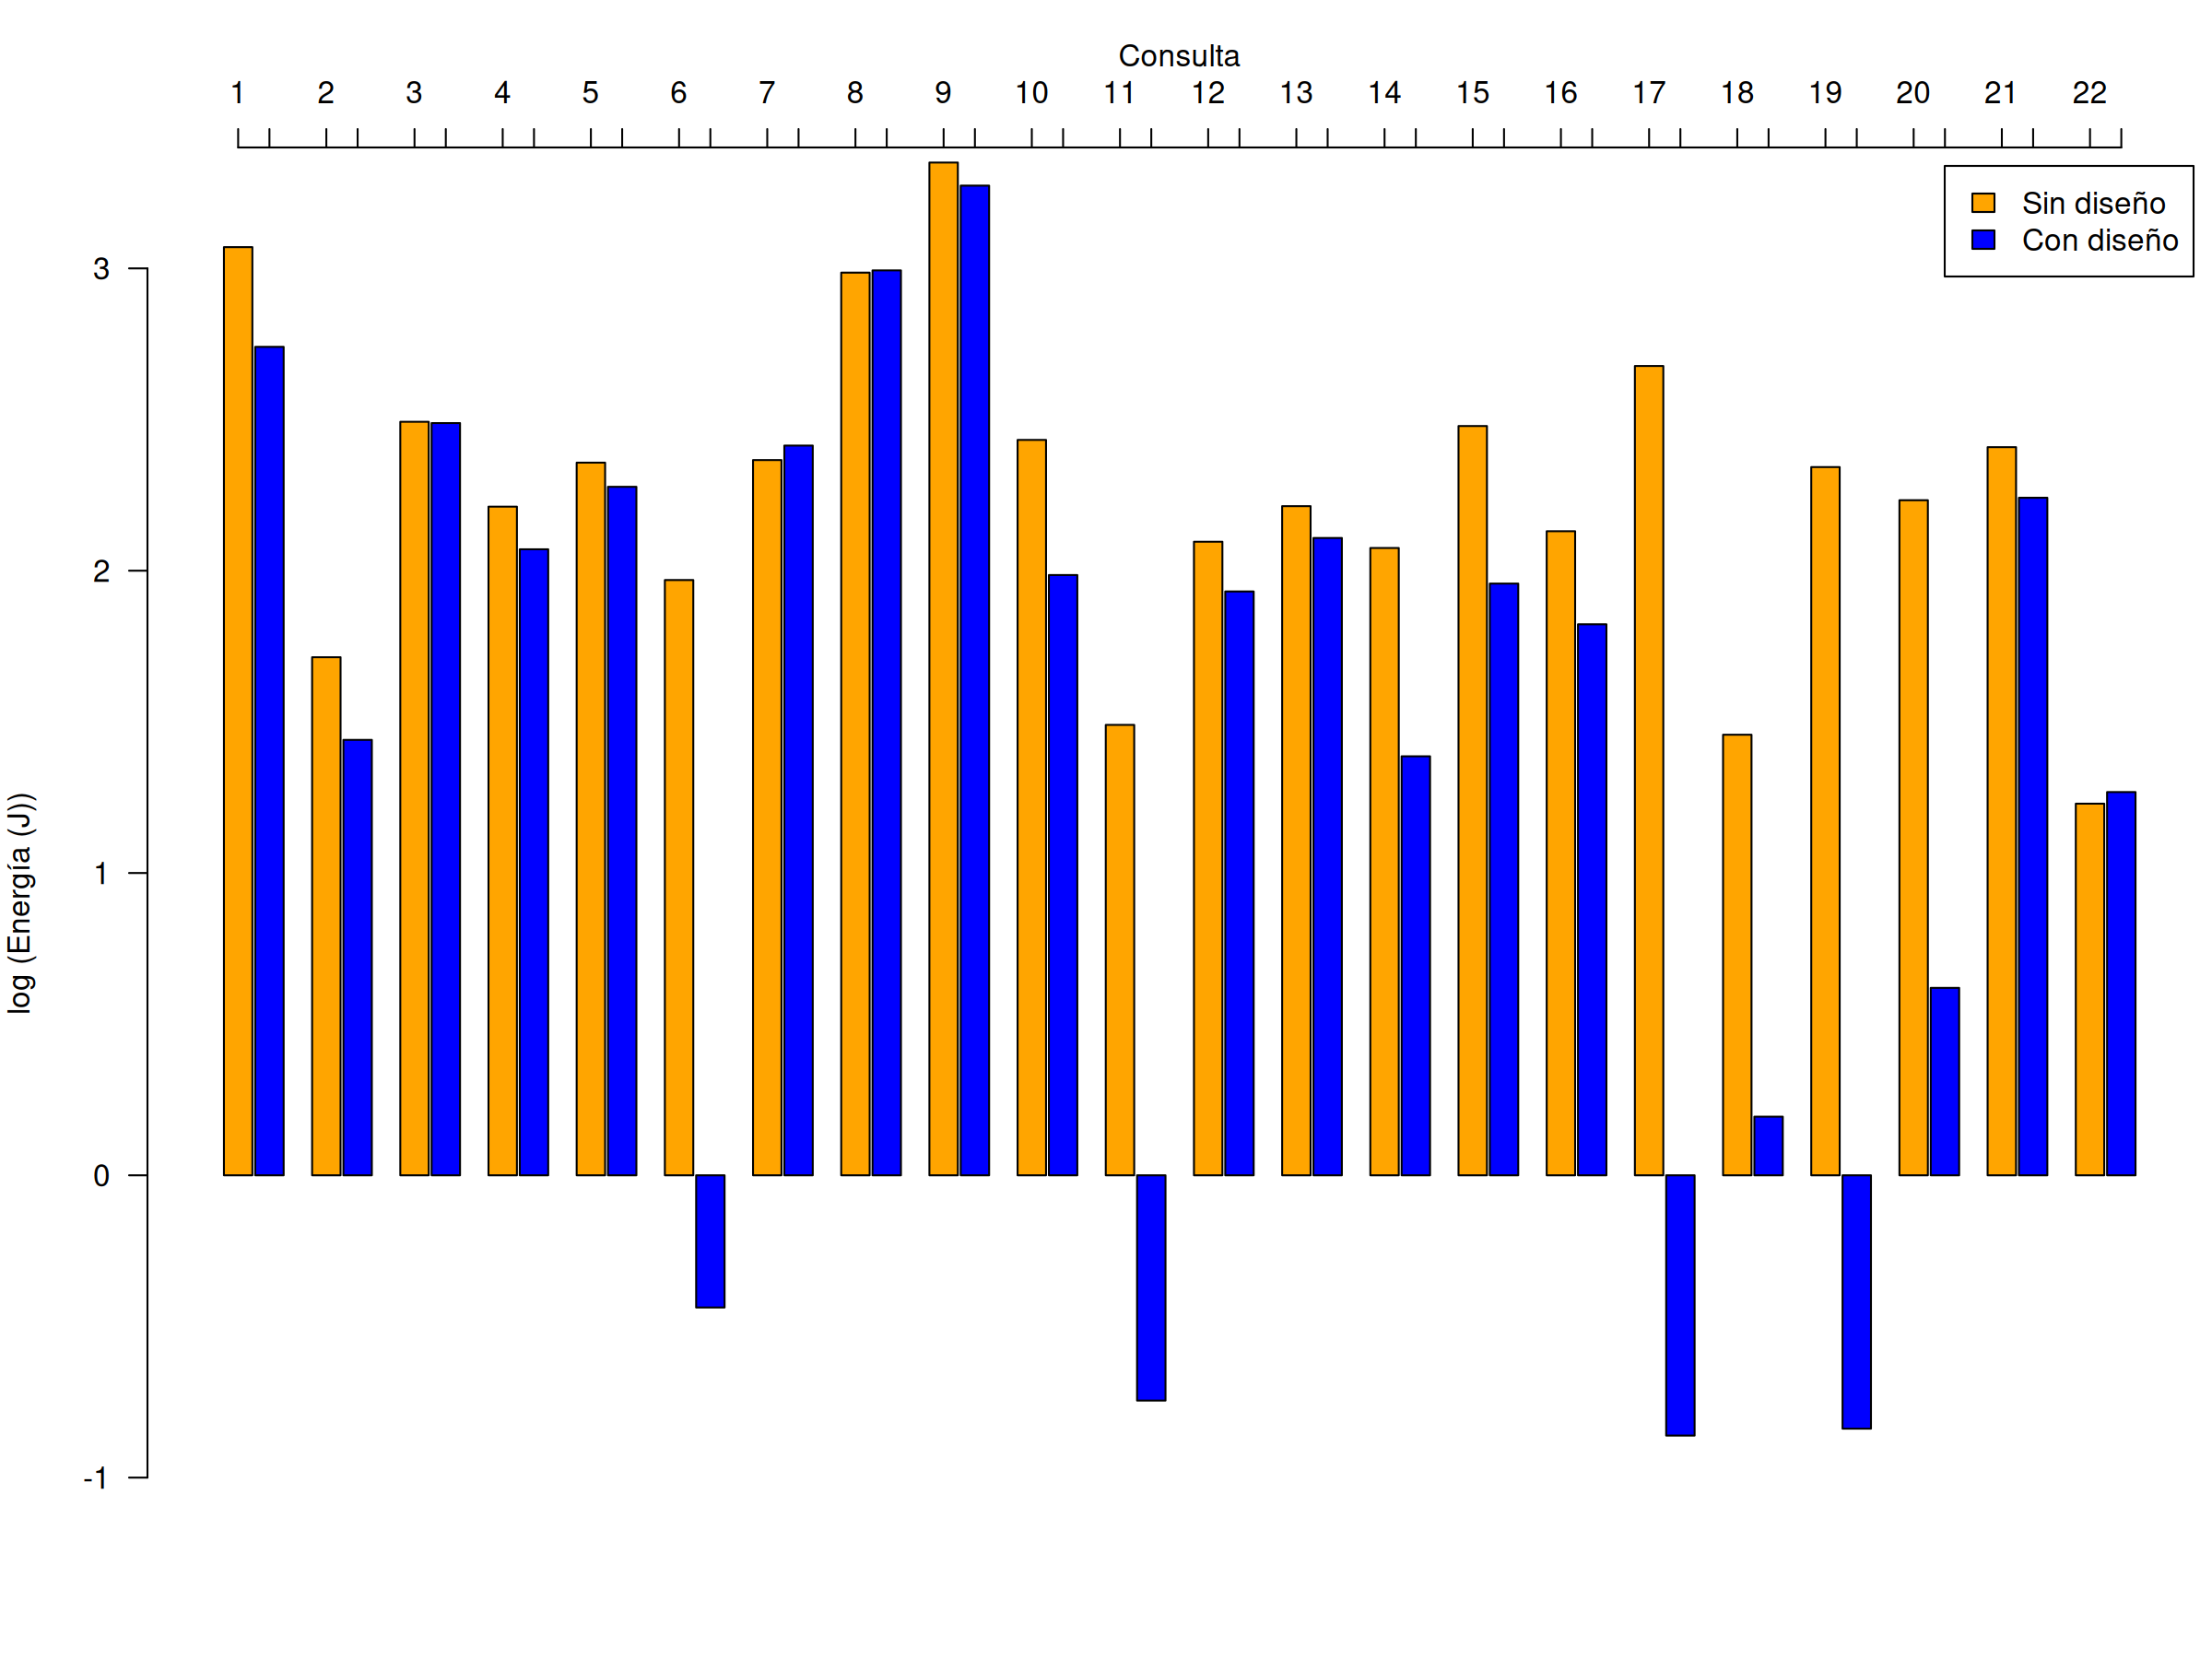
\includegraphics[width = 0.5\textwidth]{images/Neto-50G.png}
          \caption{Consumo neto por consulta 20 GB (izquierda) y 50 GB (derecha)}
          \label{fig:neto3}
        \end{figure}

        A nivel general, en las gráficas se observa una tendencia global de
        optimización energética gracias a la incorporación del diseño físico
        (ver figuras \ref{fig:neto1} y \ref{fig:neto2}). Según los planes de
        ejecución analizados, el gestor sustituye las lecturas secuenciales por
        accesos indexados directos mediante las estructuras \texttt{q21i1 ON
        lineitem (l\_orderkey, l\_suppkey, l\_receiptdate, l\_commitdate)} y
        \texttt{q04i1 ON orders (o\_orderdate, o\_orderkey, o\_orderpriority)}.
        Sin embargo, al alcanzar el escenario crítico de cincuenta gigabytes, la
        disminución del consumo energético deja de ser estadísticamente
        significativa (ver figura \ref{fig:neto3}). Este comportamiento responde
        a que, a dicha escala volumétrica, el tamaño de los índices compuestos
        supera la capacidad de la memoria RAM asignada a las cachés del sistema.
        Esto fuerza al hardware a ejecutar operaciones de lectura aleatoria
        directamente sobre el almacenamiento secundario, un cuello de botella de
        E/S que incrementa el gasto de potencia y termina por equiparar el costo
        energético del acceso indexado con el del escaneo secuencial del
        escenario base.

        Finalmente, la consulta 10 también requiere la ejecución de
        particionamiento dinámico. No obstante, los tiempos de ejecución y los
        registros de consumo sugieren que se beneficia de la optimización. En
        este escenario, el impacto positivo de la estrategia de diseño es
        evidente en casi todo el espectro volumétrico, a pesar de la limitación
        de observabilidad en el plan de ejecución global.

        La única excepción a esta tendencia de ahorro se registra en la escala
        de un gigabyte, donde la estrategia de diseño físico provocó un ligero
        incremento en el consumo energético respecto al caso base. Este fenómeno
        responde al costo fijo de inicialización y procesamiento de las
        estructuras indexadas (\textit{overhead}): a un volumen tan reducido,
        los datos residen por completo en las cachés de alta velocidad del
        procesador, haciendo que una lectura secuencial lineal sea
        energéticamente más eficiente que el patrón de acceso no contiguo del
        índice. Sin embargo, a partir de los dos gigabytes, la indexación local
        comienza a mitigar el impacto del particionamiento dinámico. Al filtrar
        los registros en el origen, el índice reduce drásticamente el volumen de
        tuplas que deben ser serializadas y transmitidas a través de la red
        durante la fase de particionamiento dinámico, lo que despliega un ahorro
        energético sostenido hasta los cincuenta gigabytes (ver figuras
        \ref{fig:neto1} a \ref{fig:neto3}).

        Por su parte, la consulta 14 exhibe un comportamiento estrechamente
        análogo. En las escalas de uno y dos gigabytes (figura \ref{fig:neto1}),
        la implementación de la estrategia de diseño físico resulta más costosa
        energéticamente que el escenario base, lo que confirma nuevamente que la
        penalización por el acceso indexado supera los beneficios de la
        optimización cuando el volumen de datos es mínimo. No obstante, a partir
        de los cinco gigabytes y hasta el escenario crítico de cincuenta
        gigabytes (figuras \ref{fig:neto2} y \ref{fig:neto3}), la tendencia se
        revierte por completo: el consumo energético disminuye de forma
        sostenida, demostrando que la estrategia logra amortizar eficazmente el
        costo del particionamiento dinámico a medida que la carga de trabajo
        escala.

        Las consultas restantes dentro del conjunto de pruebas no se discuten de
        manera individualizada en esta sección, debido a que sus factores
        críticos de rendimiento y comportamiento estructural fueron
        exhaustivamente analizados en función del tiempo de ejecución en el
        apartado anterior. Las consultas detalladas en este segmento de consumo
        neto fueron seleccionadas específicamente por presentar particularidades
        u omisiones en sus planes globales de observabilidad; no obstante, el
        resto de la carga de trabajo replica de manera homóloga las tendencias
        temporales previamente identificadas, trasladadas ahora al espectro del
        gasto de potencia absoluto.

        Con el propósito de ofrecer una visión de conjunto que condense el
        comportamiento del consumo del clúster, se introduce la tabla
        \ref{tab:consultasPorConsumo}. En esta herramienta de síntesis, las
        consultas evaluadas se categorizan formalmente en tres niveles discretos
        en función de su demanda energética neta: bajo consumo, consumo
        intermedio y alto consumo. Esta taxonomía permite identificar de un
        vistazo qué perfiles de carga representan el costo operativo crítico del
        sistema y cuáles se mantienen en umbrales de alta eficiencia, lo que
        sirve como puente hacia el análisis de correlación estadística.

        \begin{table}[H]
          \caption{Clasificación de consultas según su consumo neto}
          \begin{tabular}{| l | p{4.5cm} | p{4.5cm} | p{4.5cm} |}
            \hline Carga (GB) % \diagbox[width=6cm]{Carga (GB)}{Clase}
              &                          Poco consumo ($U < 1$)                       &                    Consumo intermedias ($1 \le U \le 10$)                &                               Consumo alto ($U > 10$)                                \\ \hline
            1 &  1, 2, 4, 6, 11, 12, 13, 15, 16, Q17(idx), 18, 19, Q20(idx), 21 y 22  &                        Q3(idx), 5, 7, Q8(idx), 10 y 14                   &                                   Q8, 9, Q17 y Q20                                   \\ \hline
            2 & 2, Q3, 4, 6, 11, 12, 13, 15, 16, 18, Q19($^\star$), Q20(idx), 21 y 22 &                        1, Q3(idx), 5, 7, 10, 14 y Q19                    &                                    8, 9, 17 y Q20                                    \\ \hline
            5 &     2, 4, 6, 11, 12, 13, Q17(idx), 18,Q19($^\star$), Q20(idx), 22     &               3, Q5(idx), Q7(idx), 10, 14, 15, 16, Q19 y 21              &                            1, Q5, Q7, 8, 9, Q17, Q19 y Q20                           \\ \hline
           10 & 2, Q6(idx), 11, Q12(idx), Q17(idx), 18, Q19($^\star$), Q20(idx), Q22  & Q4(idx), Q10(idx), Q13, Q14(idx), Q15(idx), 16, Q19($^\star$) y Q22(idx) &       1, 3, Q4, 5, Q6, 7, 8, 9, Q10, Q12, Q13(CTE), Q14, Q15, Q17, Q19, Q20 y 21     \\ \hline
           20 &   2, Q6(idx), 11, Q17(idx), Q18($^\star$), Q19($^\star$) y Q20(idx)   &                        Q12(idx), Q14(idx), Q18 y 22                      &         1, 3, 4, 5, Q6, 7, 8, 9, 10, Q12, 13, Q14, 15, 16, Q17, Q19, Q20 y 21        \\ \hline
           50 &              Q6(idx), Q11(idx), Q17(idx) y Q19($^\star$)              &                          Q18($^\star$) y Q20(idx)                        & 1, 2, 3, 4, 5, Q6, 7, 8, 9, 10, Q11, 12, 13, 14, 15, 16, Q17, Q18, Q19, Q20, 21 y 22 \\ \hline
          \end{tabular}
          \label{tab:consultasPorConsumo}
        \end{table}
      % subsection gráficos_de_barras_consumo_contra_volumen_de_datos (end)

      \subsection{Consumo del nodo coordinador} % (fold)
      \label{sub:consumo_del_nodo_coordinador}
        En cuanto al comportamiento del consumo energético del coordinador, en
        la tabla \ref{tab:consultasCoord}, se presenta la clasificación de
        consultas bajo los mismos criterios aplicados para el consumo neto. Por
        otra parte, debido a que el comportamiento de los nodos trabajadores 
        resulta análogo al desempeño del sistema, los gráficos se presentan en
        el apéndice \ref{apx:consumoWorkers}.

        \begin{table}[H]
          \caption{Clasificación de consultas según el consumo del coordinador}
          \begin{tabular}{| p{1cm} | p{6.25cm} | p{5.5cm} | p{3cm} |}
            \hline Carga (GB) % \diagbox[width=4cm]{Carga (GB)}{Clase}
              &                          Poco consumo ($U < 1$)                          &                     Consumo intermedias ($1 \le U \le 10$)                     &         Consumo alto ($U > 10$)         \\ \hline
            1 &                              1 a 7 y 10 a 22                             &                                      8 y 9                                     &                                         \\ \hline
            2 &                              1 a 7 y 10 a 22                             &                                      8 y 9                                     &                                         \\ \hline
            5 &        1 a 6, Q7, 10 a 14, Q15, 17 a 18, Q19($^\star$) y 20 a 22         &                         Q7(idx), 8, Q15(idx), 16 y Q19                         &                    9                    \\ \hline
           10 & 1 a 2, Q3, 4, Q5, 6, 11 a 12, Q13, Q14, 17 a 18, Q19($^\star$) y 20 a 22 &               Q3(idx), Q5$^\star$, 7, 10, Q14(idx), 15 a 16 y Q19              &              8, 9 y Q13(CTE)            \\ \hline
           20 &        1 a 2, 4, 6, 11 a 12, Q13, 17 a 18, Q19($^\star$) y 20 a 22       &                           3, 5, 7, Q13(CTE), 14 y Q19                          &             8 a 10 y 15 a 16            \\ \hline
           50 &          1 a 2, 4, 6, 11 a 13, 17 a 18, Q19($^\star$) y 20 a 22          & Q3(idx), Q5(idx), Q7(idx), Q8(idx), Q9(idx), Q10(idx), 14, Q15(idx) y Q16(CTE) & Q3, Q5, Q7, Q8, Q9, Q10, Q15, Q16 y Q19 \\ \hline
          \end{tabular}
          \label{tab:consultasCoord}
        \end{table}

        \begin{figure}[H]
          
\includegraphics[width = 0.49\textwidth]{images/Coordinador-1G.png}
          
\includegraphics[width = 0.49\textwidth]{images/Coordinador-2G.png}
          \caption{Consumo del nodo coordinador por consulta 1 GB (izquierda) y
          2 GB (derecha)}
          \label{fig:coord1}
        \end{figure}

        \begin{figure}[H]
          
\includegraphics[width = 0.49\textwidth]{images/Coordinador-5G.png}
          
\includegraphics[width = 0.49\textwidth]{images/Coordinador-10G.png}
          \caption{Consumo del nodo coordinador por consulta 5 GB (izquierda) y
          10 GB (derecha)}
          \label{fig:coord2}
        \end{figure}

        \begin{figure}[H]
          
\includegraphics[width = 0.49\textwidth]{images/Coordinador-20G.png}
          
\includegraphics[width = 0.49\textwidth]{images/Coordinador-50G.png}
          \caption{Consumo del nodo coordinador por consulta 20 GB (izquierda) y
          50 GB (derecha)}
          \label{fig:coord3}
        \end{figure}

        En las figuras \ref{fig:coord1}, \ref{fig:coord2} y \ref{fig:coord3}, se
        muestran los diagramas homólogos para el consumo del nodo coordinador.
        Es fundamental señalar la ausencia de una tendencia monótona en el
        comportamiento de algunas consultas al incrementar el volumen de datos.
        Esta fluctuación es atribuible a la naturaleza del diseño experimental,
        el cual se ejecutó bajo un entorno de caché caliente con un intervalo de
        muestreo de dos segundos (muy cercano al límite operativo nominal de un
        segundo de la herramienta) \cite{prometheus_best_practices,
        prometheus_configuration}.

        En ese sentido, dado que múltiples consultas se procesan en fracciones
        de segundo, fue necesario realizar decenas de miles de repeticiones para
        capturar registros válidos. Aún así, los datos obtenidos no siempre
        mantenían el mismo orden de magnitud que las mediciones previas.
        Incluso, en escenarios de alta velocidad, la ejecución finalizaba antes
        de que los sensores lograran registrar una variación en la potencia.
        Este comportamiento evidenció una limitación de observabilidad no
        prevista al inicio de la investigación, lo que fundamenta la necesidad
        de extender este estudio en el futuro mediante el uso de herramientas de
        software de mayor frecuencia o instrumentación física externa.
      % subsection consumo_del_nodo_coordinador (end)

      Por otra parte, los resultados empíricos permiten constatar que las
      estrategias de diseño físico lograron disminuir el consumo energético en
      la mayoría de las cargas evaluadas, lo que sugiere la existencia de una
      estrecha relación entre el tiempo de ejecución y la energía consumida. Las
      excepciones donde no se apreció una reducción del consumo energético se
      manifiestan en dos vertientes: las penalizaciones a baja escala (uno y dos
      gigabytes) en consultas con particionamiento dinámico como la 3, 10 y 14;
      y por otro lado, los casos globales de las consultas 8 y 9. Estos últimos
      casos corresponden a las consultas más pesadas del \textit{benchmark}, las
      cuales se vieron penalizadas por la obligación de escribir datos
      temporalmente de forma local para resolver el particionamiento dinámico.
    % section consumo_energético_neto (end)

    \section{Revisión estadística} % (fold)
    \label{sec:revision_estadistica}
      En esta sección se encuentra todo el tratamiento estadístico de los
      resultados de tiempo y consumo obtenidos.

      \subsection{Normalidad (Shapiro-Wilk)} % (fold)
      \label{sub:normalidad_shapiro_wilk}
        Para analizar estadísticamente la relación entre las variables, primero
        se descartó la normalidad de los datos con la prueba de Shapiro-Wilk.
        Los resultados de esta prueba se observan en la tabla \ref{tab:shapiro}.
        En dicha tabla se presentan los $p$-valores para las variables medidas
        en este estudio: tiempo de ejecución (tiempo) y consumo energético
        (cons.) de los nodos coordinador (coord.), trabajadores (trab.) y neto.
        Dichos $p$-valores se obtuvieron con \texttt{shapiro.test}, función
        nativa de R.

        \begin{table}[H]
          \centering
          \caption{Prueba de Shapiro-Wilk ($p$-valores)}
          \begin{tabular}{| c | c | c | c | c | c |}
            \hline
            Carga (GB) &    Tiempo   & Cons. Coord. & Cons. Trab. 1 & Cons. Trab. 2 & Cons. Neto  \\ \hline
               1 (SD)  & \num{4e-39} & \num{2e-42}  &  \num{3e-41}  &  \num{9e-42}  & \num{2e-40} \\ \hline
               1 (CD)  & \num{2e-40} & \num{5e-43}  &  \num{3e-44}  &  \num{1e-44}  & \num{2e-43} \\ \hline
               2 (SD)  & \num{6e-37} & \num{1e-43}  &  \num{4e-42}  &  \num{3e-42}  & \num{5e-42} \\ \hline
               2 (CD)  & \num{3e-41} & \num{8e-44}  &  \num{1e-43}  &  \num{4e-44}  & \num{2e-43} \\ \hline
               5 (SD)  & \num{1e-38} & \num{5e-43}  &  \num{9e-43}  &  \num{7e-43}  & \num{9e-43} \\ \hline
               5 (CD)  & \num{6e-42} & \num{3e-43}  &  \num{1e-43}  &  \num{1e-43}  & \num{2e-43} \\ \hline
              10 (SD)  & \num{6e-41} & \num{2e-42}  &  \num{8e-37}  &  \num{4e-37}  & \num{8e-38} \\ \hline
              10 (CD)  & \num{6e-43} & \num{4e-49}  &  \num{2e-49}  &  \num{2e-49}  & \num{2e-49} \\ \hline
              20 (SD)  & \num{2e-42} & \num{5e-41}  &  \num{2e-36}  &  \num{3e-36}  & \num{3e-37} \\ \hline
              20 (CD)  & \num{3e-43} & \num{6e-46}  &  \num{6e-38}  &  \num{5e-40}  & \num{2e-45} \\ \hline
              50 (SD)  & \num{2e-42} & \num{2e-38}  &  \num{9e-36}  &  \num{1e-35}  & \num{2e-36} \\ \hline
              50 (CD)  & \num{6e-44} & \num{1e-32}  &  \num{4e-38}  &  \num{2e-37}  & \num{7e-38} \\ \hline
          \end{tabular}
          \label{tab:shapiro}
        \end{table}

        Dado que los $p$-valores $<$ 0,05 se cumple que ningún dato sigue una
        distribución normal y con esto se descarta correlacionar las variables
        con el coeficiente de correlación de Pearson y en su lugar, se usa los
        de Kendall o Spearman.
      % subsection normalidad_shapiro_wilk (end)

      \subsection{Correlaciones no paramétricas: Kendall y Spearman} % (fold)
      \label{sub:correlaciones_no_paramétricas_kendall_y_spearman}
        En las tablas \ref{tab:kendall} y \ref{tab:spearman} se muestran los
        coeficientes $\tau$ y $\rho$ con sus $p$-valores para el consumo
        estimado por la integración numérica de los datos de Scaphandre y la
        ejecución de las consultas. Dichos resultados se obtuvieron con
        \texttt{cor.test}, función nativa de R.

        Los resultados de las tablas \ref{tab:kendall} y \ref{tab:spearman}
        indican que, en efecto, el consumo energético guarda una correlación
        significativa con el tiempo de ejecución para cualquier nivel de
        significancia razonablemente escogido. Por el signo de los coeficientes,
        la correlación es directa; es decir, a mayor tiempo, más consumo. Para
        la visualización de estas tendencias, en los apéndices
        \ref{apx:dispersionSD} y \ref{apx:dispersionCD} se presentan las
        gráficas de dispersión de los datos recopilados, en escala logarítmica
        en ambos ejes para mejorar la visualización de los puntos.

        \begin{table}[H]
          \centering
          \caption{Coeficientes de Kendall ($\tau$)}
          \begin{tabular}{| c | c | c | c | c |}
            \hline
            Carga (GB) &      $\tau_M(p)$     &      $\tau_1(p)$     &      $\tau_2(p)$     &      $\tau_N(p)$     \\ \hline
               1 (SD)  & 0,6222(\num{2e-126}) & 0,6603(\num{4e-142}) & 0,6720(\num{4e-147}) & 0,7117(\num{1e-164}) \\ \hline
               1 (CD)  & 0,7425(\num{4e-179}) & 0,6922(\num{6e-156}) & 0,6916(\num{1e-155}) & 0,7439(\num{8e-180}) \\ \hline
               2 (SD)  & 0,6244(\num{3e-127}) & 0,6612(\num{2e-142}) & 0,6423(\num{1e-134}) & 0,6918(\num{1e-155}) \\ \hline
               2 (CD)  & 0,6424(\num{1e-134}) & 0,4953(\num{9e-81})  & 0,4737(\num{5e-74})  & 0,5367(\num{2e-94})  \\ \hline
               5 (SD)  & 0,5783(\num{2e-109}) & 0,7144(\num{6e-166}) & 0,7244(\num{1e-170}) & 0,7812(\num{5e-198}) \\ \hline
               5 (CD)  & 0,6204(\num{2e-125}) & 0,6495(\num{2e-137}) & 0,6149(\num{3e-123}) & 0,6880(\num{7e-154}) \\ \hline
              10 (SD)  & 0,6020(\num{2e-118}) & 0,7239(\num{2e-170}) & 0,6047(\num{2e-119}) & 0,7090(\num{2e-163}) \\ \hline
              10 (CD)  & 0,5214(\num{2e-89})  & 0,6706(\num{2e-146}) & 0,6955(\num{2e-157}) & 0,7037(\num{4e-161}) \\ \hline
              20 (SD)  & 0,5181(\num{3e-88})  & 0,6536(\num{3e-139}) & 0,7344(\num{3e-175}) & 0,7296(\num{5e-173}) \\ \hline
              20 (CD)  & 0,5148(\num{4e-87})  & 0,6910(\num{2e-155}) & 0,6612(\num{2e-142}) & 0,6707(\num{2e-146}) \\ \hline
              50 (SD)  & 0,5886(\num{3e-113}) & 0,6811(\num{5e-151}) & 0,6782(\num{9e-159}) & 0,7197(\num{2e-168}) \\ \hline
              50 (CD)  & 0,5700(\num{2e-106}) & 0,7082(\num{5e-163}) & 0,7276(\num{5e-172}) & 0,7659(\num{2e-190}) \\ \hline
          \end{tabular}
          \label{tab:kendall}
        \end{table}

        \begin{table}[H]
          \centering
          \caption{Coeficientes de Spearman ($\rho$)}
          \begin{tabular}{| c | c | c | c | c |}
            \hline
            Carga (GB) &      $\rho_M(p)$     &      $\rho_1(p)$     &      $\rho_2(p)$     &      $\rho_N(p)$     \\ \hline
               1 (SD)  & 0,8030(0)            & 0,8551(0)            & 0,8723(0)            & 0,9003(0)            \\ \hline
               1 (CD)  & 0,9081(0)            & 0,8721(0)            & 0,8627(0)            & 0,9077(0)            \\ \hline
               2 (SD)  & 0,8068(0)            & 0,8554(0)            & 0,8417(0)            & 0,8807(0)            \\ \hline
               2 (CD)  & 0,8005(0)            & 0,5915(0)            & 0,5758(\num{2e-59})  & 0,6272(0)            \\ \hline
               5 (SD)  & 0,7813(0)            & 0,8865(0)            & 0,8925(0)            & 0,9323(0)            \\ \hline
               5 (CD)  & 0,8219(\num{1e-162}) & 0,8419(\num{3e-178}) & 0,8113(\num{2e-155}) & 0,8756(\num{8e-210}) \\ \hline
              10 (SD)  & 0,7657(\num{3e-128}) & 0,8921(\num{4e-229}) & 0,7857(0)            & 0,8813(0)            \\ \hline
              10 (CD)  & 0,7411(\num{6e-116}) & 0,8631(\num{2e-197}) & 0,8874(\num{2e-223}) & 0,8910(\num{8e-228}) \\ \hline
              20 (SD)  & 0,6980(\num{2e-97})  & 0,8395(\num{2e-176}) & 0,9030(\num{1e-243}) & 0,9024(\num{1e-242}) \\ \hline
              20 (CD)  & 0,7260(\num{4e-109}) & 0,8806(\num{1e-215}) & 0,8612(\num{1e-195}) & 0,8618(\num{4e-196}) \\ \hline
              50 (SD)  & 0,7579(0)            & 0,8539(0)            & 0,8503(0)            & 0,8805(0)            \\ \hline
              50 (CD)  & 0,7726(\num{6e-132}) & 0,8887(\num{5e-225}) & 0,9033(\num{5e-244}) & 0,9267(\num{6e-282}) \\ \hline
          \end{tabular}
          \label{tab:spearman}
        \end{table}
      % subsection correlaciones_no_paramétricas_kendall_y_spearman (end)

      De la revisión estadística, es evidente que la relación entre tiempo y
      consumo energético es de proporcionalidad directa; por lo tanto, reducir
      el tiempo de ejecución de una consulta con diseño físico sí reduce el
      consumo energético de la misma. Este resultado contrasta directamente con
      los postulados clásicos de Niemann \textit{et al.} \cite{niemanndoes2013},
      quienes afirman que tal correlación se rompe invariablemente en presencia
      de operaciones de E/S, lo que deriva incluso en consumos mayores para
      ejecuciones más veloces. En el escenario distribuido relacional evaluado
      en este trabajo, la evidencia empírica indica lo contrario: las
      optimizaciones físicas y lógicas que redujeron el tiempo de procesamiento
      también mitigaron la demanda energética global.

      Esta discrepancia con la literatura tradicional se explica a través del
      impacto de las estrategias de diseño físico implementadas, particularmente
      la co-locación de tablas. Al suprimir dinámicamente las transferencias de
      datos internodo a través de la red, se eliminaron los tiempos de espera
      pasivos del procesador (estados de espera de E/S). Al transformarse en un
      entorno donde el procesamiento local se ejecuta sin interrupciones, el
      consumo de potencia eléctrica se volvió directamente proporcional al
      tiempo de ocupación activa del hardware. De este modo, la estadística de
      Kendall y Spearman aporta evidencia robusta de que, bajo un diseño físico
      optimizado, la eficiencia temporal y la eficiencia energética en entornos
      distribuidos sí caminan en la misma dirección.

      Por otra parte, la presencia de una correlación estadísticamente
      significativa bajo los coeficientes de Kendall y Spearman introduce un
      matiz importante sobre los hallazgos de Lang \textit{et al.}
      \cite{langtowards2012}. Mientras que en tal estudio se argumenta que las
      operaciones de consulta se estructuran de forma asimétrica no lineal
      (donde el rendimiento transaccional y la potencia eléctrica se
      desacoplan), los datos de este trabajo revelan que la aplicación rigurosa
      de estrategias de diseño físico actúa como un agente homogeneizador. Al
      estabilizar los planes de ejecución y reducir las operaciones aleatorias,
      la asimetría postulada en \cite{langtowards2012} disminuye, lo que obliga
      a las variables de tiempo y energía a comportarse de manera directamente
      proporcional y predecible.

      Al profundizar en el análisis de sensibilidad según la escala de los
      datos, se descubrió que los coeficientes de Spearman (tabla
      \ref{tab:spearman}) y Kendall (tabla \ref{tab:kendall}) no describen una
      tendencia monótona. En lugar de registrar un comportamiento lineal o un
      crecimiento constante en la fuerza de la correlación a medida que aumenta
      el volumen de información, los coeficientes experimentan fluctuaciones y
      puntos de inflexión críticos.

      Desde una perspectiva estadística, la pérdida de monotonía en la evolución
      de los coeficientes de Spearman demuestra que la relación entre el tiempo
      de ejecución y el consumo energético sufre una alteración estructural
      profunda dependiendo de la carga. Este fenómeno valida de forma directa
      las conclusiones de Gomes \textit{et al.} \cite{gomesenergy2016}, donde se
      postula que la eficiencia energética es una variable estrictamente
      dependiente de las condiciones de contorno de la carga de trabajo, y no
      una constante del motor de bases de datos.

      El quiebre de la monotonía matemática halla su explicación física en los
      cambios de comportamiento del optimizador del gestor y en los límites del
      hardware. En escenarios de baja carga, el sistema opera bajo una dinámica
      de ráfagas rápidas controladas por la CPU; sin embargo, al escalar el
      volumen de datos a rangos donde las estructuras de diseño físico exceden
      la memoria RAM disponible, el sistema incurre en fallos de página
      (\textit{page faults}) y accesos masivos a disco. Esta transición de un
      régimen síncrono a uno dominado por la latencia de E/S destruye la
      relación monótona de las variables, lo que aporta evidencia estadística
      robusta de que el volumen de los datos actúa como un factor de quiebre
      energético en arquitecturas distribuidas.
    % section revision_estadistica (end)
  % chapter resultados_y_discusión (end)

  \newpage
  \addcontentsline{toc}{chapter}{\textbf{Conclusiones}}
  \begin{center}
    \Large \textbf{Conclusiones}
  \end{center}

  A partir de las consultas evaluadas mediante el \textit{benchmark} TPC-H —las
  cuales demostraron ser idóneas para explotar y medir las capacidades del
  sistema distribuido frente a operaciones de entrada/salida (E/S) y latencia de
  red— se evidencia que la ejecución de consultas SQL sin una estrategia de
  diseño planificada incrementa el uso de recursos computacionales y, en
  consecuencia, el consumo energético. Por el contrario, la aplicación de
  estrategias de diseño, guiada estrictamente por los planes de ejecución, logra
  optimizar tanto el tiempo de ejecución como la eficiencia energética. Este
  ahorro se produce gracias a la disminución del tiempo en que los procesos de
  las consultas permanecen activos y a la reducción drástica de las operaciones
  de E/S, las cuales representan una alta demanda de energía.

  Se demostró mediante un análisis estadístico no paramétrico (coeficientes de
  Spearman y Kendall) que, en contraposición a las teorías tradicionales para
  sistemas centralizados \cite{niemanndoes2013}, el tiempo de ejecución y el
  consumo energético guardan una correlación positiva y significativa en
  entornos distribuidos relacionales bajo la aplicación de estas estrategias de
  diseño físico. La evidencia empírica recolectada confirma que, al suprimir la
  latencia de red y optimizar los flujos lógicos, el comportamiento del hardware
  se estabiliza, logrando que la reducción del tiempo de procesamiento se
  traduzca de manera directa y estadísticamente robusta en un ahorro
  proporcional del consumo energético global del clúster.

  Sin embargo, la implementación de estas optimizaciones no es universal y
  presenta sus propias contrapartidas. Una estrategia de diseño ingenua (que
  está basada en un análisis superficial de la consulta sin considerar las
  implicaciones algorítmicas del código SQL), apresurada (sin haber estudiado el
  plan de ejecución a detalle) o impuesta de manera forzada sobre bases de datos
  pequeñas puede degradar el desempeño, ya que en volúmenes menores de
  información, los algoritmos base del gestor suelen ser más eficientes por sí
  solos. Además, aunque las estrategias de diseño físico mejoran el rendimiento
  y reducen el consumo energético a nivel de procesamiento, incrementan el uso
  de espacio en disco. Esto introduce un costo energético latente derivado de la
  necesidad de leer un mayor volumen de datos almacenados en los soportes
  físicos. Esto quiere decir que si las estructuras auxiliares creadas son más
  grandes que la memoria RAM disponible y la consulta obliga a realizar lecturas
  completas o aleatorios sobre ellas, el sistema incurre en una penalización
  constante de energía eléctrica. Específicamente, si las estructuras auxiliares
  creadas superan la capacidad de la memoria RAM disponible, el sistema incurre
  en fallos de página (\textit{page faults}) ---fenómeno en el cual el gestor se
  ve obligado a suspender la ejecución para buscar los datos faltantes en el
  almacenamiento secundario--- lo que se traduce en una penalización térmica y
  de potencia eléctrica continua sobre el hardware, destruyendo la monotonía de
  la eficiencia energética.

  Finalmente, en el contexto específico de las arquitecturas distribuidas, la
  co-locación ---técnica que consiste en almacenar los registros relacionados de
  distintas tablas en un mismo nodo físico para evitar transferencias de datos
  en la red--- de tablas emerge como factor definitivo y crítico para sostener
  el rendimiento y mitigar la latencia de red \cite{stonebraker1986case,
  dewitt1992parallel}. La relevancia de esta técnica radica en que garantiza que
  cada nodo del clúster trabaje de forma totalmente independiente
  \cite{stonebraker1986case, dewitt1992parallel} de los otros lo que justifica
  las reducciones de varios órdenes de magnitud de los tiempos de ejecución.

  A partir de este hallazgo empírico, queda propuesto como trabajo futuro
  evaluar y comparar el rendimiento de un sistema distribuido que carezca de
  co-locación frente a las capacidades de un sistema de bases de datos
  centralizado bajo escalabilidad vertical. La ruta metodológica para simular la
  co-locación requiere el rediseño y las reescritura de las consultas del
  \textit{benchmark}. Para ello, se plantea la creación de réplicas de las
  tablas modificando la clave de repartición primaria y combinándolas mediante
  operaciones de \texttt{JOIN}, de modo que se maximice la necesidad de
  redistribución de datos entre los nodos. Otra alternativa viable consiste en
  inyectar atributos sintéticos en el esquema para segmentar artificialmente los
  datos para forzar un escenario de particionamiento dinámico extremo que
  permita medir el punto de quiebre del sistema.

  Consecuentemente, el éxito en la optimización o simulación de la co-locación
  conlleva a que el rendimiento de las consultas disminuya a fracciones de
  segundo. De ahí, surge la necesidad del estudio sobre las mediciones del
  consumo energético para consultas de ese orden de magnitud, superando la
  problemática subyacente es que las herramientas utilizadas (Scaphandre y
  Prometheus) las cuales no fueron diseñadas para la alta frecuencia requerida
  por entornos distribuidos con cargas ultrarrápidas. Para resolver esta
  restricción de observabilidad que afectó la reproducibilidad en los escenarios
  de menor volumen, las futuras investigaciones deberán orientarse al estudio de
  otras herramientas de software y de hardware optimizadas para realizar
  mediciones de energía cuando las ejecuciones duran fracciones de segundo, así
  como al desarrollo de mecanismos que soporten la medición de consumo en
  ambientes distribuidos dentro de las herramientas disponibles.

  \addcontentsline{toc}{chapter}{\textbf{Referencias}}
  \bibliographystyle{IEEEtran}
  \renewcommand{\bibname}{Referencias}
  \bibliography{Refs}
  \nocite{*}

  \appendix
  \renewcommand{\thesection}{\thechapter.\arabic{section}}
  \renewcommand{\thesubsection}{\thechapter.\arabic{subsection}}
  \renewcommand{\thesubsubsection}{\thechapter.\arabic{subsubsection}}
  \renewcommand{\thefigure}{\thechapter.\arabic{figure}}
  \renewcommand{\thetable}{\thechapter.\arabic{table}}

  \chapter{TPC-H}
  \label{apx:tpch}
  \section{Diseño lógico de la base de datos} % (fold)
  \label{ssub:diseño_lógico_de_la_base_de_datos}
    Dado el diseño conceptual, se muestra el diseño lógico en modelo relacional
    \cite{transactionprocessingperformancecounciltpctpc2022} con las
    simplificaciones consideradas en la asignatura CI-3311 (Sistemas de Bases de
    Datos I):
    \begin{itemize}
      \item \texttt{Region(\underline{regionkey}, name, comment)}.
      \item \texttt{Nation(\underline{nationkey}, name, $\overset{
        \texttt{region}}{\overline{\texttt{regionkey}}}$, comment)}.
      \item \texttt{Part(\underline{partkey}, name, mfgr, brand, type, size,
      container, retailprice, \\comment)}.
      \item \texttt{Customer(\underline{custkey}, name, address,
      $\overset{\texttt{nation}}{\overline{\texttt{nationkey}}}$, phone,
      acctbal, mktsegment, \\comment)}.
      \item \texttt{Supplier(\underline{suppkey}, name, address,
      $\overset{\texttt{nation}}{\overline{\texttt{nationkey}}}$, phone,
      acctbal, comment)}.
      \item \texttt{Orders(\underline{orderkey}, $\overset{
        \texttt{customer}}{\overline{\texttt{custkey}}}$, orderstatus,
        totalprice, orderpriority, clerk, \\shippriority, comment)}.
      \item \texttt{Lineitem(\underline{$\overset{\texttt{orders}}{
        \overline{\texttt{orderkey}}}$, linenumber}, $\overset{\texttt{
        partsupp}}{\overline{\texttt{partkey},\ \texttt{supplier}}}$,
        quantity, extendedprice, \\
        discount, tax, returnflag, linestatus, shipdate, commitdate,
        receiptdate, \\shipinstruct, shipmode, comment)}.
      \item \texttt{Partsupp(\underline{$\overset{\texttt{part}}{
        \overline{\texttt{partkey}}}$, $\overset{\texttt{supplier}}{
        \overline{\texttt{suppkey}}}$}, availqty, supplycost, comment)}.
    \end{itemize}
  % section diseño_lógico_de_la_base_de_datos (end)

  \section{Consultas} % (fold)
  \label{sec:consultas}
    A continuación se presenta una lista con una breve descripción conceptual
    de cada consulta del \textit{benchmark} TPC-H
    \cite{transactionprocessingperformancecounciltpctpc2022}.
      \begin{enumerate}
        \item Informe del resumen de precios: informa sobre la cantidad de
        negocios facturados, enviados y devueltos.
        \item Proveedor de costo mínimo: encuentra el proveedor que se debe
        seleccionar para realizar un pedido de una pieza determinada en una
        región específica.
        \item Prioridad de envío: recupera los 10 pedidos no enviados con el
        mayor valor.
        \item Comprobación de prioridad de pedidos: determina el desempeño
        del sistema de prioridad de pedidos y proporciona una evaluación de
        la satisfacción del cliente.
        \item Volumen de proveedores locales: indica el volumen de ingresos
        generados a través de proveedores locales.
        \item Pronóstico de cambios en los ingresos: cuantifica el aumento
        de ingresos que se habría producido al eliminar ciertos descuentos a
        nivel de toda la empresa en un rango porcentual determinado en un
        año determinado.
        \item Volumen de envíos: determina el valor de las mercancías
        enviadas entre ciertos países para facilitar la renegociación de los
        contratos de envío.
        \item Cuota de mercado nacional: determina cómo ha cambiado la cuota
        de mercado de un país determinado dentro de una región específica a
        lo largo de dos años para un tipo de pieza determinado.
        \item Medida de utilidad por tipo de producto: determina la utilidad
        obtenida de una línea de piezas determinada, desglosada por país del
        proveedor y año.
        \item Informe de devoluciones: identifica a los clientes que podrían
        tener problemas con las piezas que se les envían.
        \item Identificación de stock importante: encuentra el subconjunto
        más importante del stock de los proveedores en un país determinado.
        \item Modos de envío y prioridad de pedidos: determina si la
        selección de modos de envío más económicos afecta negativamente a
        los pedidos de prioridad crítica, al provocar que los clientes
        reciban más piezas después de la fecha límite.
        \item Distribución de clientes: busca relaciones entre los clientes
        y el tamaño de sus pedidos.
        \item Efecto de promoción: monitoriza la respuesta del mercado a una
        promoción, como anuncios de televisión o una campaña especial.
        \item Proveedor principal: identifica al proveedor principal para
        recompensarlo, aumentar su negocio o identificarlo para un
        reconocimiento especial.
        \item Relación piezas/proveedor: determina cuántos proveedores
        pueden suministrar piezas con atributos determinados. Puede
        utilizarse, por ejemplo, para determinar si hay suficientes
        proveedores para piezas con gran demanda.
        \item Ingresos por pedidos de pequeña cantidad: determina la pérdida
        promedio de ingresos anuales si no se surtieran pedidos de pequeñas
        cantidades de ciertas piezas. Esto puede reducir los gastos
        generales al concentrar las ventas en envíos más grandes.
        \item Cliente de gran volumen: clasifica a los clientes según si han
        realizado un pedido de gran cantidad. Los pedidos de gran cantidad
        se definen como aquellos cuya cantidad total supera un cierto nivel.
        \item Ingresos descontados: informa los ingresos brutos descontados
        atribuidos a la venta de piezas seleccionadas, gestionadas de una
        manera específica. Esta consulta es un ejemplo de código que podría
        generarse programáticamente mediante una herramienta de minería de
        datos.
        \item Promoción potencial de piezas: identifica a los proveedores de
        un país en particular que han seleccionado piezas que podrían ser
        candidatas a una oferta promocional.
        \item Proveedores con pedidos en espera: identifica a ciertos
        proveedores que no pudieron enviar las piezas requeridas a tiempo.
        \item Oportunidad de venta global: identifica zonas geográficas
        donde hay clientes con probabilidades de realizar una compra.
      \end{enumerate}

      \begin{figure}[H]
        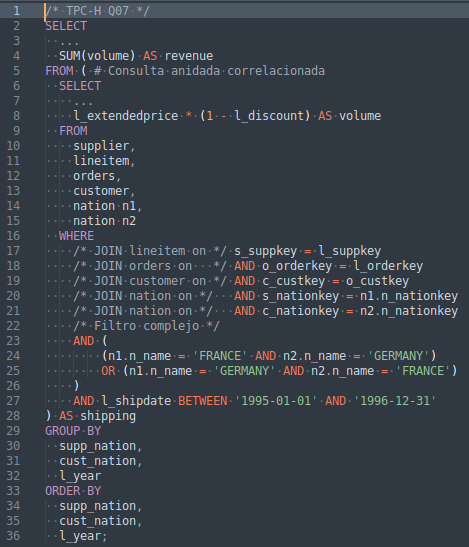
\includegraphics[width = 0.33\textwidth]{images/Q7.png}
        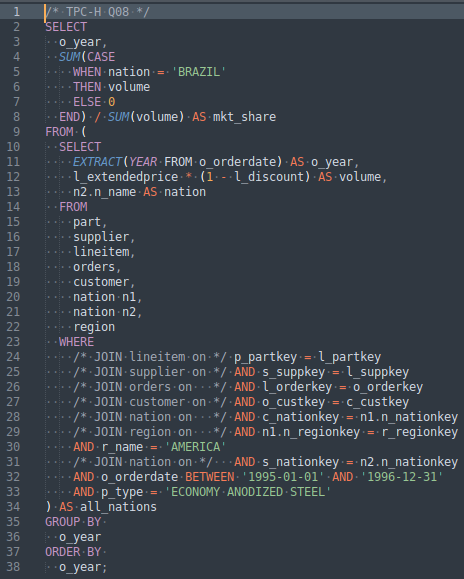
\includegraphics[width = 0.33\textwidth]{images/Q8.png}
        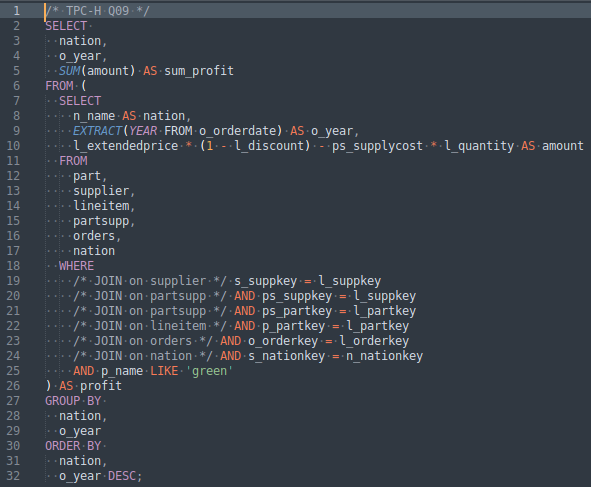
\includegraphics[width = 0.33\textwidth]{images/Q9.png}
        \caption{Consultas inherentemente pesadas}
        \label{fig:pesadas}
      \end{figure}

      En la figura \ref{fig:pesadas} se muestran las operaciones inherentemente
      costosas para el gestor y para la consulta. Sólo las tablas
      \texttt{nation} (veinticinco filas), \texttt{region} (cinco filas) y
      \textit{supplier} (10 000S filas con S igual al número de gigabytes de la
      base de datos)

      \begin{figure}
        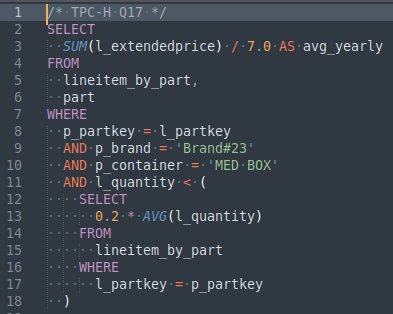
\includegraphics[width = 0.5\textwidth]{images/Q17.png}
        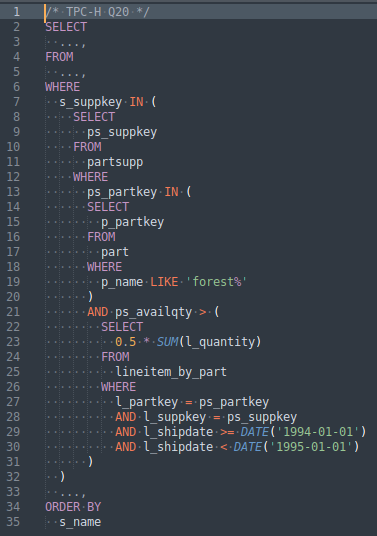
\includegraphics[width = 0.5\textwidth]{images/Q20.png}
        \caption{Consultas Q17 y Q20}
        \label{fig:Q17yQ20}
      \end{figure}

      \begin{figure}[H]
        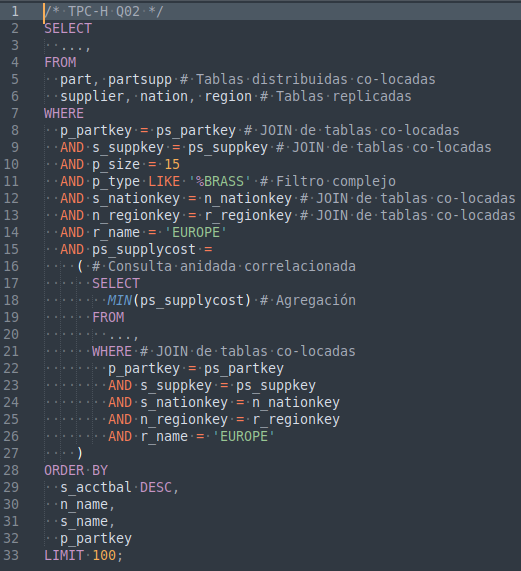
\includegraphics[width = 0.33\textwidth]{images/Q2.png}
        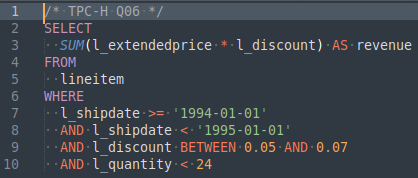
\includegraphics[width = 0.33\textwidth]{images/Q6.png}
        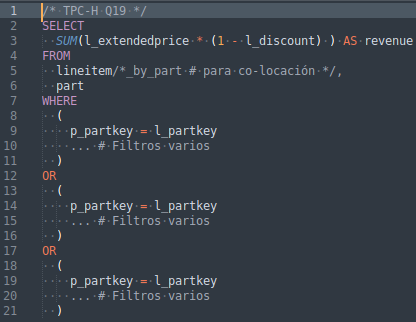
\includegraphics[width = 0.33\textwidth]{images/Q19.png}
        \caption{Consultas 2, 6, 19}
        \label{fig:AunRapidas}
      \end{figure}

      \begin{figure}[H]
        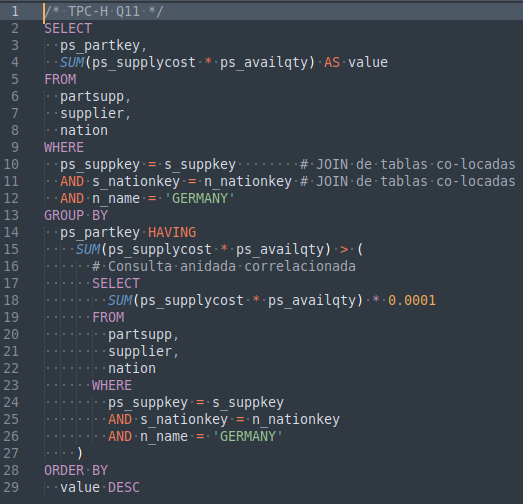
\includegraphics[width = 0.33\textwidth]{images/Q11.png}
        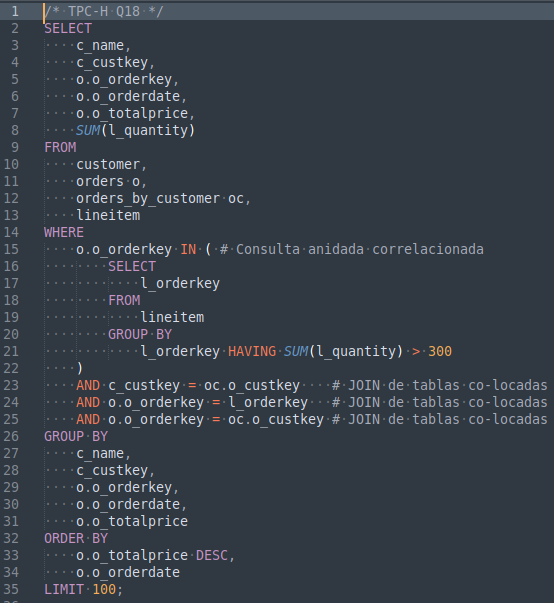
\includegraphics[width = 0.33\textwidth]{images/Q18.png}
        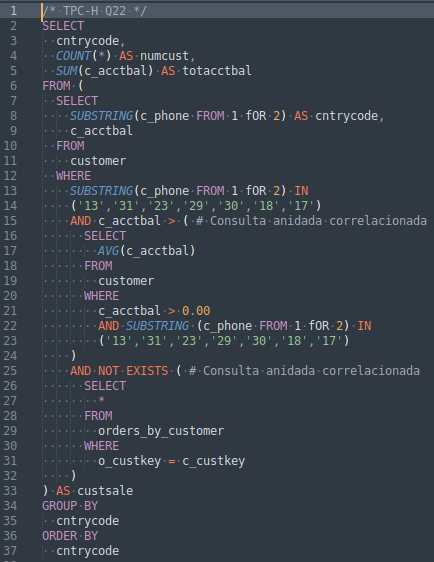
\includegraphics[width = 0.33\textwidth]{images/Q22.png}
        \caption{Consultas 11, 18, 22}
        \label{fig:intermedias}
      \end{figure}

      \begin{figure}[H]
        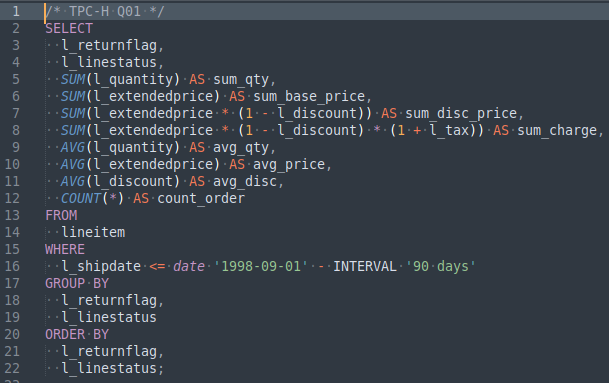
\includegraphics[width = 0.33\textwidth]{images/Q1.png}
        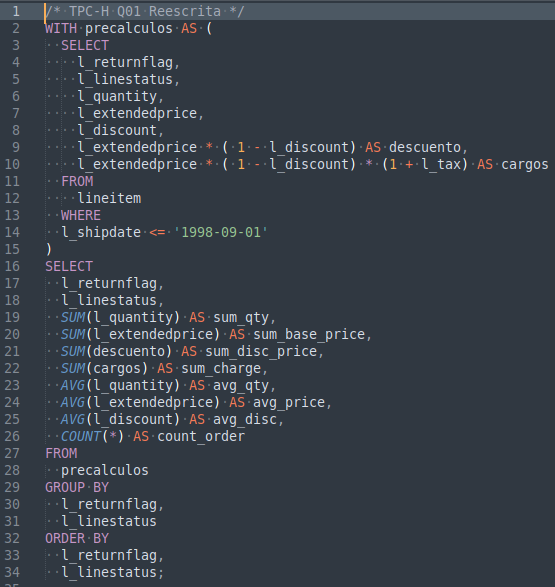
\includegraphics[width = 0.33\textwidth]{images/Q01.png}
        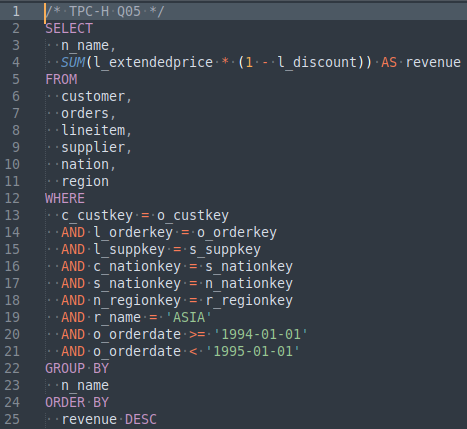
\includegraphics[width = 0.33\textwidth]{images/Q5.png}
        \caption{Consultas 1 (original, izquierda y reescrita, centro), 5 y 21}
        \label{fig:insig1}
      \end{figure}

      \begin{figure}[H]
        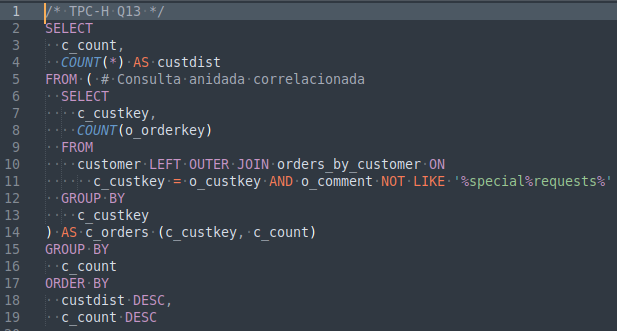
\includegraphics[width = 0.5\textwidth]{images/Q13.png}
        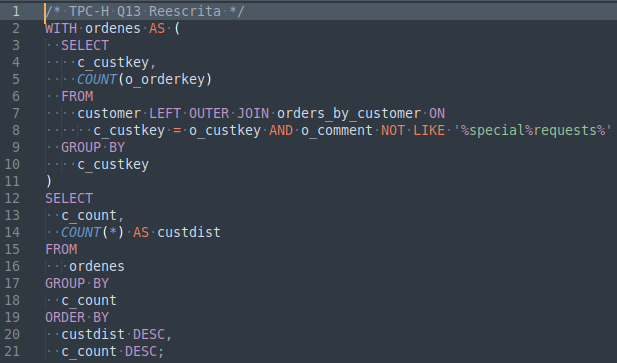
\includegraphics[width = 0.5\textwidth]{images/Q013.png}
        \caption{Consulta 13}
        \label{fig:insig2}
      \end{figure}

      \begin{figure}[H]
        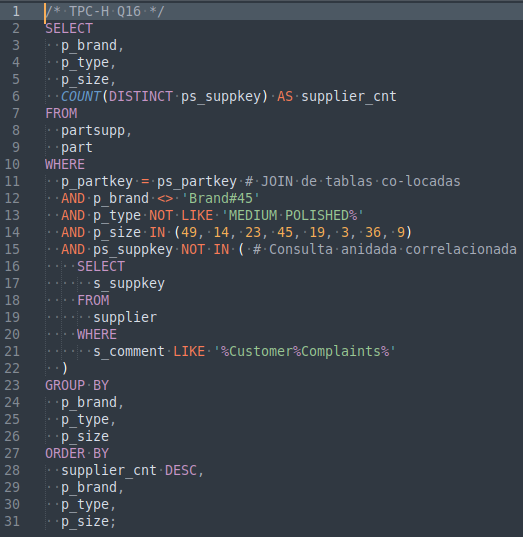
\includegraphics[width = 0.5\textwidth]{images/Q16.png}
        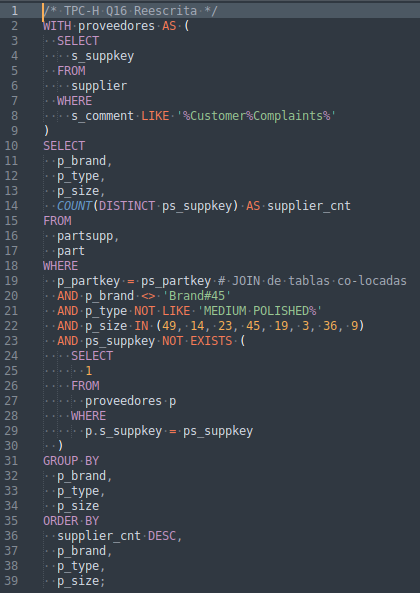
\includegraphics[width = 0.5\textwidth]{images/Q016.png}
        \caption{Consulta 16}
        \label{fig:insig3}
      \end{figure}

      \begin{figure}[H]
        \centering
        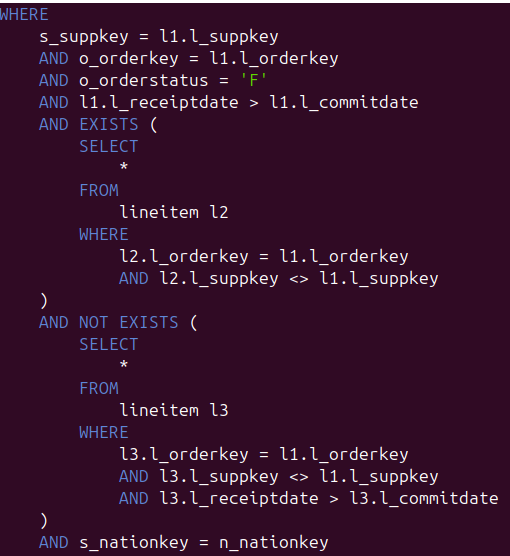
\includegraphics[width=0.5\textwidth]{images/joins.png}
        \caption{\texttt{JOIN} en Q21}
        \label{fig:joins}
      \end{figure}

        \begin{figure}[H]
          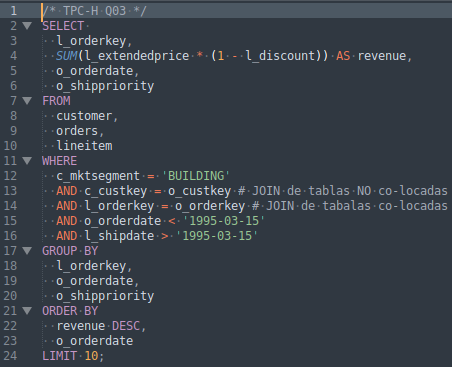
\includegraphics[width = 0.5\textwidth]{images/Q3.png}
          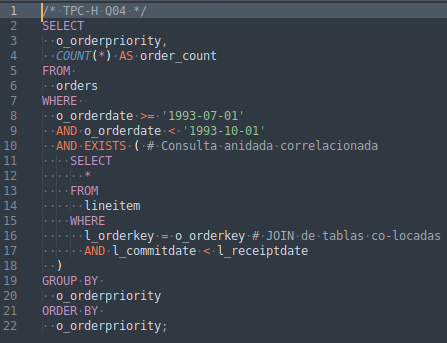
\includegraphics[width = 0.5\textwidth]{images/Q4.png}
          \caption{Consultas 3 y 4}
          \label{fig:pocoConsumo1}
        \end{figure}

        \begin{figure}[H]
          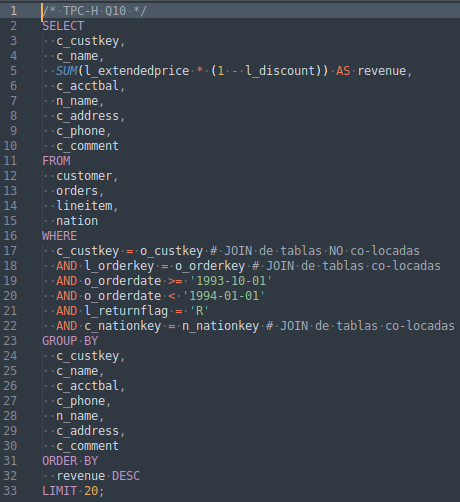
\includegraphics[width = 0.5\textwidth]{images/Q10.png}
          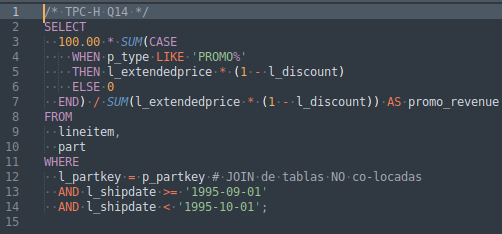
\includegraphics[width = 0.5\textwidth]{images/Q14.png}
          \caption{Consultas 10 y 14}
          \label{fig:pocoConsumo2}
        \end{figure}
  % section consultas (end)

  \chapter{Instalación de herramientas}
  \label{apx:herramientas}
    \section{Scaphandre} % (fold)
    \label{sec:scaphandre}
      \lstinputlisting[language = Bash]{scripts/scaphandre.sh}
    % section scaphandre (end)

    \section{Prometheus} % (fold)
    \label{sec:prometheus1}
      La instalación es directa y vía \texttt{apt}:

      \lstinputlisting[language = Bash]{scripts/prometheus.sh}

      Se debe modificar el archivo \texttt{/etc/prometheus/prometheus.yml}
      de forma que se vea así:

      \lstinputlisting{scripts/prometheus.yml}

      Para,finalmente, reiniciar el servicio mediante \texttt{systemctl}:

      \lstinputlisting{scripts/prometheus-check.sh}

      La herramienta \texttt{promtool} permite verificar la sintaxis del
      archivo de configuración editado para garantizar que el reinicio del
      servicio sea exitoso. Sin embargo, como medida adicional, se sugiere
      verificar el estado del servicio con el último paso.
    % section prometheus1 (end)

    \section{Jq} % (fold)
    \label{sec:jq}
      Este es un procesador de archivos \texttt{JSON} de CLI. Su instalación
      también es directa mediante \texttt{apt-get}:

      \lstinputlisting[language = Bash]{scripts/jq.sh}

      Su función es la de tomar las métricas recolectadas por Prometheus y
      procesarlas en entradas legibles para humanos.
    % section jq (end)

    \section{Dbgen de TPC-H} % (fold)
    \label{sec:dbgen_de_tpc_h}
      Es el generador de datos aleatorios para el \textit{benchmark} TPC-H.
      Se obtiene todo el lote mediante descarga directa en su sitio
      oficial\footnote[1]{https:\/\/www.tpc.org\/tpc\_documents\_current\_versions\/current\_specifications5.asp}.
      La descarga requiere que el usuario llene un formulario en señal de
      aceptación de los términos y condiciones de uso. El formulario puede
      llenarse de forma segura con los datos de la afiliación a la Universidad
      Simón Bolívar, o a otra institución de ser preciso. Este formulario hará
      que se envíe un correo electrónico con el enlace de descarga a la
      dirección que el usuario suministró.

      Una vez descargado el archivo se deben seguir los siguientes pasos
      para completar la instalación solamente en uno de los computadores:

      \lstinputlisting[language = Bash]{scripts/dbgen.sh}
    % section dbgen_de_tpc_h (end)

    \section{Configuración de clústeres} % (fold)
    \label{sec:configuración_de_clústeres}
      Para la instalación de un clúster de bases de datos relacionales como
      PostgreSQL se necesitan extensiones de estos gestores que funcionen como
      \textit{middlewares} y versiones de los mismos gestores que sean
      compatibles. El \textit{middleware} de PostgreSQL es Citus y el proceso de
      instalación es:

      \lstinputlisting[language = Bash]{scripts/citus.sh}

      El nombre $<$\texttt{base-de-datos}$>$ es libre para el usuario con la
      única condición de que no haya sido usado previamente.

      Cuando la creación ha sido exitosa, se le debe indicar a Citus quién
      es el nodo administrador (\textit{manager}) y quiénes son los nodos
      trabajadores (\textit{workers}). Para ello, primero, hay que conectar
      los nodos del clúster mediante el archivo de configuración
      \texttt{/etc/postgresql/16/main/pg\_hba.conf}. En este archivo hay que
      añadir líneas al final de él, una por cada ordenador a utilizar:

      \lstinputlisting{scripts/pg_hba.conf}

      Cada $<$\texttt{IP}$>$ corresponde a cada ordenador y esto permite que
      todos los ordenadores puedan enviarse resultados parciales de las
      consultas de ser requerido. Luego, dentro de \texttt{psql} se debe
      indicar la identidad de cada nodo a Citus:

      \lstinputlisting[language = Bash]{scripts/citus1.sh}

      Esto finaliza la configuración del clúster.
    % section configuración_de_clústeres (end)
  % chapter instalación_de_herramientas (end)

  % \chapter{Estudio con 100 GB}
  % \label{apx:mac}
  % % chapter estudio_con_100_gb

  \chapter{Medias y desviaciones estándar del consumo energético por nodos}
  \label{apx:nodos}
    \section{Consumo nodo coordinador} % (fold)
    \label{sec:consumo_nodo_coordinador}
      \begin{table}[H]
        \caption{Sin diseño}
        \footnotesize
        \begin{tabular}{| c | c | c | c | c | c | c |}
          \hline \diagbox[width=4cm]{Consulta}{Carga (GB)}
              &       1      &       2      &       5      &      10      &       20       &       50       \\ \hline
           Q1 & 0,0(2)       & 0(5)         & \num{0(1)e1} & \num{0(2)e1} & \num{0(2)e1}   & \num{0(2)e1}   \\ \hline
           Q2 & 0,001(1)     & 0,002(7)     & 0,00(1)      & 0,00(1)      & 0,0(5)         & 0(7)           \\ \hline
           Q3 & 0,1(6)       & 0,0(1)       & 0(2)         & 1(3)         & 7(9)           & \num{2(1)e1}   \\ \hline
           Q4 & 0,004(2)     & 0,003(8)     & 0,00(2)      & 0(2)         & 0(3)           & 0(4)           \\ \hline
           Q5 & 0(1)         & 0(2)         & \num{0(1)e1} & 1(5)         & 4(7)           & \num{2(1)e1}   \\ \hline
           Q6 & 0,00(1)      & 0,00(2)      & 0,00(1)      & 0(2)         & 0(2)           & 0(2)           \\ \hline
           Q7 & 0(1)         & 0,6(9)       & \num{0(1)e1} & 1(3)         & 3(3)           & \num{1(1)e1}   \\ \hline
           Q8 & 0(4)         & 3(7)         & \num{1(2)e1} & \num{1(2)e1} & \num{3(2)e1}   & \num{1,4(3)e2} \\ \hline
           Q9 & 0(9)         & \num{1(2)e1} & \num{2(2)e1} & \num{5(2)e1} & \num{1,1(3)e2} & \num{2,9(5)e2} \\ \hline
          Q10 & 0,2(3)       & 0,1(5)       & 1(1)         & 3(3)         & 14(5)          & \num{7(1)e1}   \\ \hline
          Q11 & 0,002(3)     & 0,002(4)     & 0,00(1)      & 0,0(2)       & 0(1)           & 0(2)           \\ \hline
          Q12 & 0,003(2)     & 0,00(1)      & 0,01(1)      & 0(2)         & 0(2)           & 0(2)           \\ \hline
          Q13 & 0,002(3)     & 0,00(1)      & 0,004(9)     & 0(6)         & 0(9)           & \num{0(2)e1}   \\ \hline
          Q14 & 0,0(4)       & 0,0(2)       & 0(2)         & 0(2)         & 5(2)           & 9(6)           \\ \hline
          Q15 & 0,010(6)     & 0,12(1)      & 1(4)         & 4(3)         & 11(5)          & 36(9)          \\ \hline
          Q16 & 0,008(3)     & 0,014(5)     & 1,9(1)       & 7,1(2)       & 23(7)          & \num{7(1)e1}   \\ \hline
          Q17 & 0(7)         & \num{0(1)e1} & \num{0(2)e1} & 0(2)         & 0(2)           & \num{0(6)e1}   \\ \hline
          Q18 & 0,002(4)     & 0,003(4)     & 0,00(1)      & 0,00(2)      & 0(2)           & 0(9)           \\ \hline
          Q19 & 0,0(4)       & 0(1)         & 0,00(1)      & 4(3)         & 6(4)           & 27(8)          \\ \hline
          Q20 & \num{0(1)e1} & \num{0(1)e1} & 2(4)         & 0(4)         & 0(6)           & 0(9)           \\ \hline
          Q21 & 0,002(4)     & 0,00(1)      & \num{0(2)e1} & 0(3)         & 0(4)           & 0(6)           \\ \hline
          Q22 & 0,002(1)     & 0,003(1)     & 0,006(7)     & 0,04(8)      & 0,01(4)        & 0,1(4)         \\ \hline
        \end{tabular}
      \end{table}

      \begin{table}[H]
        \caption{Con diseño}
        \footnotesize
        \begin{tabular}{| c | c | c | c | c | c | c |}
          \hline \diagbox[width=4cm]{Consulta}{Carga (GB)}
              &     1    &       2      &       5      &      10      &       20       &      50      \\ \hline
           Q1 & 0,0(2)   & 0,01(2)      & 0(9)         & 0(9)         & \num{0(1)e1}   & 0(8)         \\ \hline
           Q2 & 0,001(3) & 0,002(2)     & 0,002(6)     & 0,00(2)      & 0,00(1)        & 0(3)         \\ \hline
           Q3 & 0,0(5)   & 0,1(6)       & 0(2)         & \num{0(1)e1} & \num{0(1)e1}   & \num{4(2)e1} \\ \hline
           Q4 & 0,001(4) & 0,001(4)     & 0,01(8)      & 0,0(5)       & 0(4)           & 0(9)         \\ \hline
           Q5 & 0,1(9)   & 0,1(6)       & 0(1)         & \num{0(2)e1} & 4(8)           & \num{5(1)e1} \\ \hline
           Q6 & 0,001(2) & 0,001(3)     & 0,002(3)     & 0,002(9)     & 0,002(8)       & 0,0(2)       \\ \hline
           Q7 & 0,6(5)   & 0,7(8)       & 1(3)         & \num{0(1)e1} & \num{0(2)e1}   & \num{5(2)e1} \\ \hline
           Q8 & 0(3)     & \num{0(1)e1} & \num{1(2)e1} & \num{1(2)e1} & \num{3(2)e1}   & \num{5(3)e1} \\ \hline
           Q9 & 0(7)     & \num{1(2)e1} & \num{2(2)e1} & \num{5(2)e1} & \num{1,1(2)e2} & \num{6(8)e1} \\ \hline
          Q10 & 0,4(6)   & 0,3(4)       & 0,7(7)       & 3(1)         & 13(9)          & \num{5(2)e1} \\ \hline
          Q11 & 0,001(2) & 0,001(2)     & 0,026(9)     & 0,00(2)      & 0,07(8)        & 0,01(7)      \\ \hline
          Q12 & 0,001(2) & 0,002(5)     & 0,00(1)      & 0,001(9)     & 0(4)           & 0(4)         \\ \hline
          Q13 & 0,01(8)  & 0,1(4)       & 0,005(9)     & \num{0(2)e4} & \num{1(2)e1}   & \num{0(4)e1} \\ \hline
          Q14 & 0,1(1)   & 0(4)         & 0,1(4)       & 2(1)         & 4(3)           & 3(9)         \\ \hline
          Q15 & 0,006(2) & 0,0(6)       & 1,2(5)       & 4(1)         & 13(8)          & 4(8)         \\ \hline
          Q16 & 0,007(2) & 0,01(1)      & 2,48(5)      & 6,3(3)       & 18946(5)       & \num{0(2)e1} \\ \hline
          Q17 & 0,001(4) & \num{0(1)e1} & 0,001(3)     & 0,001(3)     & 0,002(9)       & 0,002(6)     \\ \hline
          Q18 & 0,002(6) & 0,00(1)      & 0,001(7)     & 0,00(2)      & 0,00(2)        & 0(3)         \\ \hline
          Q19 & 0,001(2) & 0,001(4)     & 0,003(7)     & 0,00(1)      & 0,00(1)        & 0,001(4)     \\ \hline
          Q20 & 0,00(2)  & 0,003(3)     & 0,00(1)      & 0,01(2)      & 0,01(3)        & 0(2)         \\ \hline
          Q21 & 0,00(1)  & 0,00(2)      & 0,01(6)      & 0(2)         & 0(3)           & 0(3)         \\ \hline
          Q22 & 0,002(2) & 0,0018(8)    & 0,02(7)      & 0,0(1)       & 0,03(7)        & 0,02(6)      \\ \hline
        \end{tabular}
      \end{table}
    % section consumo_nodo_coordinador (end)

    \section{Consumo nodo trabajador 1} % (fold)
    \label{sec:consumo_nodo_trabajador_1}
      \begin{table}[H]
        \caption{Sin diseño}
        \footnotesize
        \begin{tabular}{| c | c | c | c | c | c | c |}
          \hline \diagbox[width=4cm]{Consulta}{Carga (GB)}
              &       1      &        2       &        5        &       10       &       20       &        50       \\ \hline
           Q1 & 0,1(2)       & 2(5)           & \num{3(1)e1}    & \num{9(2)e1}   & \num{2,2(2)e2} & \num{5,9(2)e2}  \\ \hline
           Q2 & 0,012(1)     & 0,016(7)       & 0,02(1)         & 0,01(1)        & 0,1(5)         & 27(7)           \\ \hline
           Q3 & 0,5(6)       & 0,3(1)         & 1(2)            & 22(3)          & 51(9)          & \num{1,5(1)e2}  \\ \hline
           Q4 & 0,025(2)     & 0,045(8)       & 0,05(2)         & 13(2)          & 32(3)          & 82(4)           \\ \hline
           Q5 & 0(1)         & 1(2)           & \num{1(1)e1}    & 43(5)          & 85(7)          & \num{1,1(1)e2}  \\ \hline
           Q6 & 0,04(1)      & 0,04(2)        & 0,04(1)         & 6(2)           & 15(2)          & 45(2)           \\ \hline
           Q7 & 0(1)         & 0,9(9)         & \num{1(1)e1}    & 23(3)          & 40(3)          & \num{1,10(1)e2} \\ \hline
           Q8 & 0(4)         & 0(7)           & \num{3(2)e1}    & \num{9(2)e1}   & \num{1,8(2)e2} & \num{4,3(3)e2}  \\ \hline
           Q9 & 0(9)         & \num{4(2)e1}   & \num{1,2(2)e2}  & \num{2,1(2)e2} & \num{4,1(3)e2} & \num{1,01(5)e3} \\ \hline
          Q10 & 0,4(3)       & 0,4(5)         & 2(1)            & 18(3)          & 34(5)          & \num{1,0(1)e2}  \\ \hline
          Q11 & 0,014(3)     & 0,014(4)       & 0,02(1)         & 0,1(2)         & 0(1)           & 17(2)           \\ \hline
          Q12 & 0,042(2)     & 0,05(1)        & 0,04(1)         & 10(2)          & 22(2)          & 59(2)           \\ \hline
          Q13 & 0,017(3)     & 0,01(1)        & 0,023(9)        & 2(6)           & 14(9)          & \num{8(2)e1}    \\ \hline
          Q14 & 0,5(4)       & 0,4(2)         & 2(2)            & 10(2)          & 20(2)          & 56(6)           \\ \hline
          Q15 & 0,026(6)     & 0,05(1)        & 4(4)            & 22(3)          & 43(5)          & 116(9)          \\ \hline
          Q16 & 0,010(3)     & 0,012(5)       & 0,0(1)          & 0,2(2)         & 4(7)           & \num{2(1)e1}    \\ \hline
          Q17 & 0(7)         & \num{1,4(1)e2} & \num{1,06(2)e3} & 8(2)           & 27(2)          & \num{2,6(6)e2}  \\ \hline
          Q18 & 0,024(4)     & 0,025(4)       & 0,02(1)         & 0,02(2)        & 2(2)           & 15(9)           \\ \hline
          Q19 & 0,4(4)       & 0(1)           & 0,02(1)         & 19(3)          & 35(4)          & 93(8)           \\ \hline
          Q20 & \num{0(1)e1} & \num{2,3(1)e2} & 4(4)            & 15(4)          & 40(6)          & 116(9)          \\ \hline
          Q21 & 0,046(4)     & 0,04(1)        & \num{1,61(2)e3} & 19(3)          & 42(4)          & 129(6)          \\ \hline
          Q22 & 0,011(1)     & 0,013(4)       & 0,2(4)          & 0,1(3)         & 2(3)           & 6(6)            \\ \hline
        \end{tabular}
      \end{table}

      \begin{table}[H]
        \caption{Con diseño}
        \footnotesize
        \begin{tabular}{| c | c | c | c | c | c | c |}
          \hline \diagbox[width=4cm]{Consulta}{Carga (GB)}
              &     1    &        2       &        5       &       10       &       20       &        50       \\ \hline
           Q1 & 0,1(2)   & 0,05(2)        & 8(9)           & 47(9)          & \num{1,0(1)e2} & 289(8)          \\ \hline
           Q2 & 0,007(3) & 0,009(2)       & 0,007(6)       & 0,03(2)        & 0,02(1)        & 16(3)           \\ \hline
           Q3 & 0,6(5)   & 0,5(6)         & 1(2)           & \num{1(1)e1}   & \num{5(1)e1}   & \num{1,6(2)e1}  \\ \hline
           Q4 & 0,008(4) & 0,017(4)       & 0,03(8)        & 0,1(5)         & 19(4)          & 77(9)           \\ \hline
           Q5 & 0,6(9)   & 0,5(6)         & 1(1)           & \num{2(2)e1}   & 133(8)         & \num{9(1)e1}    \\ \hline
           Q6 & 0,008(2) & 0,009(3)       & 0,005(3)       & 0,012(9)       & 0,012(8)       & 0,1(2)          \\ \hline
           Q7 & 0,6(5)   & 0,8(8)         & 2(3)           & \num{1(1)e1}   & \num{3(2)e1}   & \num{1,3(2)e2}  \\ \hline
           Q8 & 0(3)     & \num{1(1)e1}   & \num{4(2)e1}   & \num{9(2)e1}   & \num{1,7(2)e2} & \num{4,5(3)e2}  \\ \hline
           Q9 & 0(7)     & \num{4(2)e1}   & \num{1,2(2)e2} & \num{2,0(2)e2} & \num{4,1(2)e2} & \num{9,82(8)e2} \\ \hline
          Q10 & 0,5(6)   & 0,4(4)         & 1,2(7)         & 3(1)           & 11(9)          & \num{5(2)e1}    \\ \hline
          Q11 & 0,006(2) & 0,008(2)       & 0,017(9)       & 0,01(2)        & 0,04(8)        & 0,05(7)         \\ \hline
          Q12 & 0,010(2) & 0,041(5)       & 0,01(1)        & 0,010(9)       & 3(4)           & 53(4)           \\ \hline
          Q13 & 0,04(8)  & 0,1(4)         & 0,022(9)       & \num{0(2)e4}   & \num{2(2)e1}   & \num{4(4)e1}    \\ \hline
          Q14 & 0,4(1)   & 0(4)           & 0,5(4)         & 1(1)           & 3(3)           & 11(9)           \\ \hline
          Q15 & 0,010(2) & 0,1(6)         & 0,4(5)         & 2(1)           & 12(8)          & 26(8)           \\ \hline
          Q16 & 0,010(2) & 0,01(1)        & 0,03(5)        & 0,3(3)         & 23(5)          & \num{3(2)e1}    \\ \hline
          Q17 & 0,006(4) & \num{1,4(1)e2} & 0,005(3)       & 0,004(3)       & 0,011(9)       & 0,018(6)        \\ \hline
          Q18 & 0,020(6) & 0,02(1)        & 0,006(7)       & 0,01(2)        & 0,01(2)        & 1(3)            \\ \hline
          Q19 & 0,006(2) & 0,006(4)       & 0,013(7)       & 0,01(1)        & 0,01(1)        & 0,021(4)        \\ \hline
          Q20 & 0,01(2)  & 0,009(3)       & 0,01(1)        & 0,01(2)        & 0,02(3)        & 0(2)            \\ \hline
          Q21 & 0,05(1)  & 0,05(2)        & 0,04(6)        & 14(2)          & 34(3)          & 87(3)           \\ \hline
          Q22 & 0,009(2) & 0,014(4)       & 0,04(8)        & 1(2)           & 1(2)           & 10(8)           \\ \hline
        \end{tabular}
      \end{table}
    % section consumo_nodo_trabajador_1 (end)

    \section{Consumo nodo trabajador 2} % (fold)
    \label{sec:consumo_nodo_trabajador_2}
      \begin{table}[H]
        \caption{Sin diseño}
        \footnotesize
        \begin{tabular}{| c | c | c | c | c | c | c |}
          \hline \diagbox[width=4cm]{Consulta}{Carga (GB)}
              &       1      &        2       &        5        &       10       &       20       &       50       \\ \hline
           Q1 & 0,1(4)       & 4(7)           & \num{3(1)e1}    & \num{1,0(1)e2} & \num{2,3(2)e2} & \num{5,9(3)e2} \\ \hline
           Q2 & 0,013(2)     & 0,019(6)       & 0,02(2)         & 0,01(1)        & 0(1)           & 25(8)          \\ \hline
           Q3 & 0,6(7)       & 0,3(1)         & 2(3)            & \num{2(1)e1}   & 59(9)          & \num{1,4(2)e2} \\ \hline
           Q4 & 0,027(3)     & 0,047(7)       & 0,04(1)         & 9(4)           & 33(5)          & 81(7)          \\ \hline
           Q5 & 0(1)         & 1(2)           & 10(8)           & \num{4(2)e1}   & 94(7)          & 103(8)         \\ \hline
           Q6 & 0,04(1)      & 0,04(1)        & 0,1(2)          & 6(4)           & 15(1)          & 48(5)          \\ \hline
           Q7 & 0(1)         & 2(4)           & 5(6)            & 13(8)          & 47(7)          & \num{1,1(1)e2} \\ \hline
           Q8 & 0(3)         & 10(8)          & \num{2(1)e1}    & \num{8(2)e1}   & \num{1,9(2)e1} & \num{4,1(4)e2} \\ \hline
           Q9 & \num{0(1)e1} & \num{3(2)e1}   & \num{1,0(3)e2}  & \num{2,1(3)e2} & \num{4,6(2)e1} & \num{9,4(6)e2} \\ \hline
          Q10 & 0,6(6)       & 0,7(7)         & 2(2)            & \num{1(1)e1}   & 32(5)          & \num{1,0(1)e2} \\ \hline
          Q11 & 0,014(3)     & 0,014(5)       & 0,03(2)         & 0,0(1)         & 0,03(2)        & \num{1(1)e1}   \\ \hline
          Q12 & 0,040(2)     & 0,05(1)        & 0,1(5)          & 10(3)          & 21(2)          & 66(5)          \\ \hline
          Q13 & 0,017(2)     & 0,02(1)        & 0,04(1)         & 1(3)           & 15(9)          & \num{9(2)e1}   \\ \hline
          Q14 & 0,5(5)       & 0,7(6)         & 1(1)            & 12(3)          & 22(3)          & 54(7)          \\ \hline
          Q15 & 0,03(1)      & 0,3(9)         & 5(5)            & \num{2(2)e1}   & 53(7)          & \num{1,5(2)e1} \\ \hline
          Q16 & 0,012(3)     & 0,02(2)        & 0,04(7)         & 1(2)           & \num{1(1)e1}   & \num{4(2)e1}   \\ \hline
          Q17 & 0(9)         & \num{1,5(1)e2} & \num{1,25(2)e3} & 15(5)          & 62(6)          & 212(8)         \\ \hline
          Q18 & 0,025(6)     & 0,028(6)       & 0,03(1)         & 0,03(3)        & 4(4)           & 14(8)          \\ \hline
          Q19 & 0,4(4)       & 0(1)           & 0,03(1)         & 15(5)          & 35(4)          & 100(8)         \\ \hline
          Q20 & \num{0(1)e1} & \num{2,3(1)e2} & 3(3)            & 9(2)           & 15(7)          & 54(4)          \\ \hline
          Q21 & 0,045(6)     & 0,05(1)        & \num{1,66(2)e3} & \num{2(1)e1}   & 45(5)          & 127(9)         \\ \hline
          Q22 & 0,011(1)     & 0,012(5)       & 1(2)            & 0,1(2)         & 0,2(6)         & 11(5)          \\ \hline
        \end{tabular}
      \end{table}

      \begin{table}[H]
        \caption{Con diseño}
        \footnotesize
        \begin{tabular}{| c | c | c | c | c | c | c |}
          \hline \diagbox[width=4cm]{Consulta}{Carga (GB)}
              &     1    &        2       &        5       &       10       &       20       &       50       \\ \hline
           Q1 & 0,1(1)   & 3(5)           & 10(9)          & \num{4(2)e1}   & \num{1,0(2)e2} & \num{2,6(2)e2} \\ \hline
           Q2 & 0,008(2) & 0,009(2)       & 0,011(9)       & 0,03(2)        & 0,03(1)        & 12(1)          \\ \hline
           Q3 & 0,5(3)   & 0,5(3)         & 1(1)           & 9(7)           & \num{5(2)e1}   & \num{1,4(2)e2} \\ \hline
           Q4 & 0,009(2) & 0,019(5)       & 0,02(2)        & 4(2)           & 1(2)           & 40(5)          \\ \hline
           Q5 & 0,7(7)   & 0,6(8)         & 2(2)           & \num{1(1)e1}   & \num{5(3)e1}   & \num{1,0(1)e2} \\ \hline
           Q6 & 0,009(2) & 0,010(3)       & 0,02(1)        & 0,02(1)        & 0,015(7)       & 0,2(5)         \\ \hline
           Q7 & 0,9(8)   & 0,7(9)         & 4(6)           & 6(9)           & \num{3(1)e1}   & \num{1,2(3)e2} \\ \hline
           Q8 & 0(3)     & \num{1(1)e1}   & \num{3(1)e1}   & \num{8(2)e1}   & \num{1,8(2)e2} & \num{5,3(3)e2} \\ \hline
           Q9 & 0(9)     & \num{3(1)e1}   & \num{1,1(3)e2} & \num{1,9(2)e2} & \num{4,4(3)e2} & \num{9(1)e2}   \\ \hline
          Q10 & 0,5(4)   & 0,4(3)         & 1,4(8)         & 3(2)           & 7(4)           & \num{4(2)e1}   \\ \hline
          Q11 & 0,008(2) & 0,009(1)       & 0,05(4)        & 0,01(2)        & 0,014(7)       & 0,025(5)       \\ \hline
          Q12 & 0,011(3) & 0,033(7)       & 0,01(2)        & 0,010(9)       & 3(3)           & 32(7)          \\ \hline
          Q13 & 0,04(7)  & 0,1(6)         & 0,03(1)        & \num{2(9)e3}   & \num{2(1)e1}   & \num{9(2)e1}   \\ \hline
          Q14 & 0,6(7)   & 0(5)           & 0,5(3)         & 1,1(7)         & 1,9(9)         & 10(7)          \\ \hline
          Q15 & 0,010(3) & 0,1(5)         & 1(1)           & 2(1)           & \num{2(1)e1}   & \num{6(3)e1}   \\ \hline
          Q16 & 0,011(3) & 0,011(3)       & 0,02(3)        & 1(1)           & 1(2)           & \num{4(2)e1}   \\ \hline
          Q17 & 0,006(4) & \num{1,5(1)e1} & 0,006(4)       & 0,006(3)       & 0,01(1)        & 0,018(6)       \\ \hline
          Q18 & 0,023(7) & 0,03(1)        & 0,008(8)       & 0,01(2)        & 0,03(5)        & 0(2)           \\ \hline
          Q19 & 0,007(3) & 0,006(2)       & 0,018(9)       & 0,01(1)        & 0,02(2)        & 0,023(5)       \\ \hline
          Q20 & 0,01(1)  & 0,009(3)       & 0,01(1)        & 0,01(2)        & 0,003(2)       & 3(6)           \\ \hline
          Q21 & 0,046(9) & 0,04(1)        & 1(3)           & \num{1(1)e1}   & 33(4)          & 87(5)          \\ \hline
          Q22 & 0,011(2) & 0,014(3)       & 0,02(2)        & 0,3(9)         & 0,1(4)         & 9(5)           \\ \hline
        \end{tabular}
      \end{table}
    % section consumo_nodo_trabajador_2 (end)
  % chapter medias_y_desviaciones_estandar_del_consumo_energetico_por_nodos

  \chapter{Consumo nodos trabajadores}
  \label{apx:consumoWorkers}
    En las figuras siguientes (\ref{fig:worker1_1} a \ref{fig:coord3}) se
    presentarán los diagramas de barras para el consumo energético de cada
    consulta con cada volumen de datos. Luego se dará un análisis global de las
    tendencias observadas en cada gráfica. En el apéndice \ref{apx:nodos} se
    muestran las tablas con las medias y las desviaciones estándar.

    \begin{figure}[H]
      
\includegraphics[width = 0.5\textwidth]{images/Worker1-1G.png}
      
\includegraphics[width = 0.5\textwidth]{images/Worker1-2G.png}
      \caption{Consumo del trabajador uno por consulta 1 GB (izquierda) y 2 GB
      (derecha)}
      \label{fig:worker1_1}
    \end{figure}

    En la figura \ref{fig:worker1_1} se puede apreciar la siguiente división de
    consultas según si el consumo es poco, moderado o alto: para un gigabyte,
    consumen poco las consultas 1, 2, 3, 4, 5, 6, 7, 10, 11, 12, 13, 14, 15, 16,
    Q17(idx), 18, 19, Q20(idx), 21 y 22; mientras que para dos gigabytes son
    Q1(CTE), 2, 3, 4, 5, 6, 7, 10, 11, 12, 13, Q14, 15, 16, 18, 19,
    Q20(idx), 21, 22. Las que presentan consumo moderado son: la 8 para un
    gigabyte y Q1, Q8, Q14(idx) para dos gigabytes. Las de consumo alto son:
    9, Q17 y Q20 para un giga y Q8(idx), 9, 17 y Q20 para dos.

    \begin{figure}[H]
      
\includegraphics[width = 0.5\textwidth]{images/Worker1-5G.png}
      
\includegraphics[width = 0.5\textwidth]{images/Worker1-10G.png}
      \caption{Consumo del trabajador uno por consulta 5 GB (izquierda) y 10 GB
      (derecha)}
      \label{fig:worker1_2}
    \end{figure}

    De la figura \ref{fig:worker1_2} se tiene la clasificación de consultas como
    se sigue: para cinco gigabytes, consumen poco las consultas 2, 4, 6, 11, 12,
    13, Q14(idx), Q15(idx), 16, Q17(idx), 18, Q19($^\star$), Q20(idx)
    y 22 mientras que para diez gigabytes son 2, Q4(idx), Q6(idx), 11,
    Q12(idx), 16, Q17(idx), 18, Q19($^\star$), Q20(idx) y 22. Las
    consultas de consumo moderado son: Q1(CTE), 3, Q5(idx), 7, 10, Q13,
    Q14, Q19 para cinco gigabytes mientras que para diez gigabytes son Q6,
    Q7(idx), Q10(idx), Q12, Q13, 14, Q15(idx) y Q17. Finalmente, las de
    consumo alto son: Q1, Q5, 8, 9, Q17 y Q20 para cinco gigabytes y 1, 3, Q4, 5,
    Q7, 8, 9, Q10, Q13(CTE), Q15, Q19, Q20 y 21 para diez.

    \begin{figure}[H]
      
\includegraphics[width = 0.5\textwidth]{images/Worker1-20G.png}
      
\includegraphics[width = 0.5\textwidth]{images/Worker1-50G.png}
      \caption{Consumo del trabajador uno por consulta 20 GB (izquierda) y 50 GB
      (derecha)}
      \label{fig:worker1_3}
    \end{figure}

    De la figura \ref{fig:worker1_3} se sigue la siguiente clasificación de las
    consultas: para veinte gigabytes, consumen poco las consultas 2, Q6(idx),
    11, Q17(idx), Q18($^\star$), Q19($^\star$) y Q20(idx) y para cincuenta
    gigabytes son Q6(idx), Q11(idx), Q17(idx), Q19($^\star$) y Q20(idx).
    Para las que exhiben consumo moderado son: Q12(idx), Q14(idx),
    Q15(idx), Q16, Q18 y 22 para veinte gigabytes mientras que para cincuenta
    gigabytes son Q14(idx), Q18($^\star$) y 22. Por último, las consultas de
    consumo alto son: 1, 3, 4, 5, Q6, 7, 8, 9, 10, Q12, 13, Q14, Q15,
    Q16(CTE), Q17, Q18, Q19, Q20 y 21 para veinte gigabytes y para cincuenta
    gigabytes se incluyen además Q11, Q12(idx), Q15(idx) y Q16.

    Análogamente para el segundo trabajador, en la figura \ref{fig:worker2_1} se
    tiene la clasificación: 1, 2, 3, 4, 5, 6, 7, 10, 11, 12, 13, 14, 15, 16,
    Q17(idx), 18, 19, Q20(idx), 21 y 22 son las que consumen poco con un
    gigabyte mientras que con dos son 2, 3, 4, Q5(idx), 6, Q7(idx), 10,
    11, 12, 13, Q14, 15, 16, 18, 19, Q20(idx), 21 y 22. Las de consumo
    moderado son 8 para un gigabyte y 1, Q5, Q7, Q8 y Q14(idx) para dos.
    Finalmente, las de consumo alto son: 9, Q17 y Q20 para un giga mientras que
    para dos son Q8(idx), 9, 17 y Q20.

    \begin{figure}[H]
      
\includegraphics[width = 0.5\textwidth]{images/Worker2-1G.png}
      
\includegraphics[width = 0.5\textwidth]{images/Worker2-2G.png}
      \caption{Consumo del trabajador dos por consulta 1 GB (izquierda) y 2 GB
      (derecha)}
      \label{fig:worker2_1}
    \end{figure}

    De la figura \ref{fig:worker2_2} se desprende la siguiente clasificación:
    las que consumen poco son 2, 4, 6, 11, 12, 13, Q14(idx), Q15(idx), 16,
    Q17(idx), 18, Q19($^\star$), Q20(idx), 21 y 22 para cinco gigabytes y
    para diez gigabytes son 2, Q6(idx), 11, Q12(idx), Q16(CTE),
    Q17(idx), 18, Q19($^\star$), Q20(idx) y 22. Las consultas de consumo
    enegético moderado son Q1(CTE), 3, 5, 7, 10, Q14, Q15 y Q19 para cinco
    gigabytes y con diez gigabytes son Q3(idx), 4, Q6, Q7(idx), 10, Q12, Q13,
    14, Q15(idx), Q16 y Q20. Y las de consumo alto son Q1, 8, 9, Q17 y Q20
    para cinco gigabytes y para diez son 1, Q3, 5, Q7, 8, 9, Q13(CTE), Q15, Q17,
    Q19 y 21.

    \begin{figure}[H]
      
\includegraphics[width = 0.5\textwidth]{images/Worker2-5G.png}
      
\includegraphics[width = 0.5\textwidth]{images/Worker2-10G.png}
      \caption{Consumo del trabajador dos por consulta 5 GB (izquierda) y 10 GB
      (derecha)}
      \label{fig:worker2_2}
    \end{figure}

    En la figura \ref{fig:worker2_3} se observa la clasificación: 2, Q4(idx),
    Q6(idx), 11, Q17(idx), Q18($^\star$), Q19($^\star$), Q20(idx) y 22 son
    las consultas que consumen poca energía para la carga de veinte gigabytes y
    para cincuenta gigabytes son Q6(idx), Q11(idx), Q17(idx), Q18($^\star$) y
    Q19($^\star$). Las de consumo moderado son Q10(idx), Q12(idx),
    Q14(idx), 16 y Q18 con veinte gigabytes y Q14(idx), Q20(idx) y 22 para
    cincuenta. Finalmente, las consultas de consumo alto son 1, 3, Q4, 5, Q6, 7,
    8, 9, Q10, Q12, 13, Q14, 15, Q17, Q19, Q20 y 21 para veinte gigabytes y para
    cincuenta son 1, 2, 3, 4, 5, Q6, 7, 8, 9, 10, Q11, 12, 13, Q14, 15, 16, Q17,
    Q18, Q19, Q20 y 21.

    \begin{figure}[H]
      
\includegraphics[width = 0.5\textwidth]{images/Worker2-20G.png}
      
\includegraphics[width = 0.5\textwidth]{images/Worker2-50G.png}
      \caption{Consumo del trabajador dos por consulta 20 GB (izquierda) y 50 GB
      (derecha)}
      \label{fig:worker2_3}
    \end{figure}
  % chapter consumo_nodos_trabajadores

  \chapter{Gráficos de dispersión sin diseño}
  \label{apx:dispersionSD}

    \section{Consumo neto} % (fold)
    \label{sec:consumo_neto}
    
    \begin{figure}[H]
      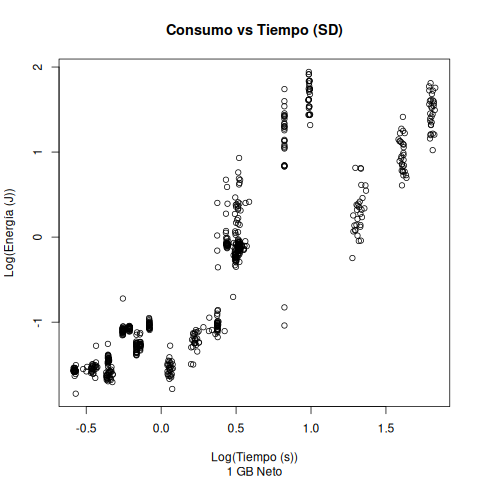
\includegraphics[width = 0.5\textwidth]{images/Dispersión-Neto-1G-SD.png}
      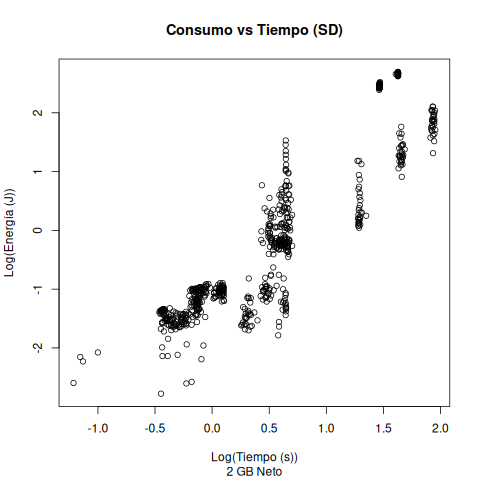
\includegraphics[width = 0.5\textwidth]{images/Dispersión-Neto-2G-SD.png}
      \caption{Gŕaficos de dispersión de consumo neto para 1 GB y 2 GB}
      \label{fig:dispersionNeto1SD}
    \end{figure}

    \begin{figure}[H]
      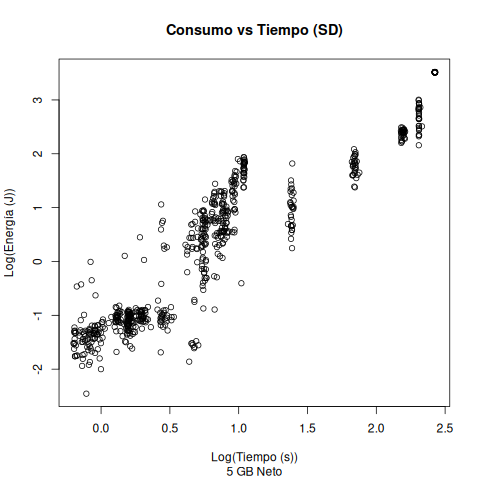
\includegraphics[width = 0.5\textwidth]{images/Dispersión-Neto-5G-SD.png}
      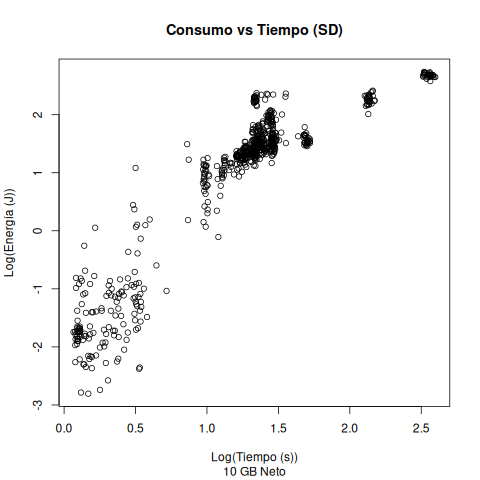
\includegraphics[width = 0.5\textwidth]{images/Dispersión-Neto-10G-SD.png}
      \caption{Gŕaficos de dispersión de consumo neto para 5 GB y 10 GB}
      \label{fig:dispersionNeto2SD}
    \end{figure}

    \begin{figure}[H]
      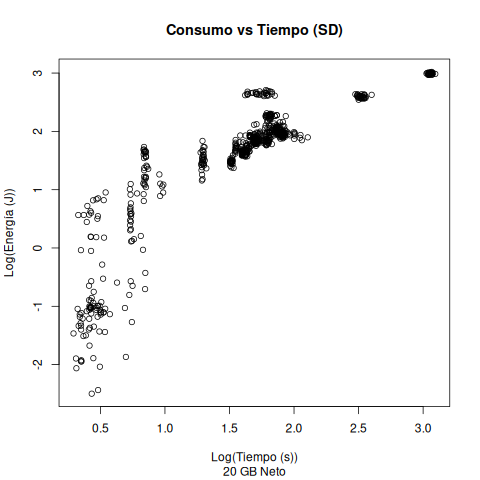
\includegraphics[width = 0.5\textwidth]{images/Dispersión-Neto-20G-SD.png}
      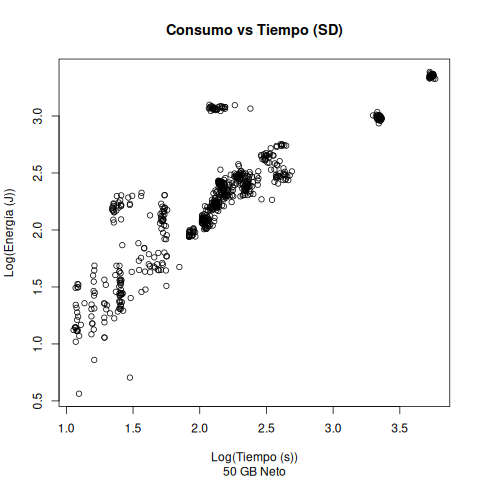
\includegraphics[width = 0.5\textwidth]{images/Dispersión-Neto-50G-SD.png}
      \caption{Gŕaficos de dispersión de consumo neto para 20 GB y 50 GB}
      \label{fig:dispersionNeto3SD}
    \end{figure}

    % section consumo_neto (end)

    \section{Consumo trabajador 1} % (fold)
    \label{sec:consumo_trabajador_1}

    \begin{figure}[H]
      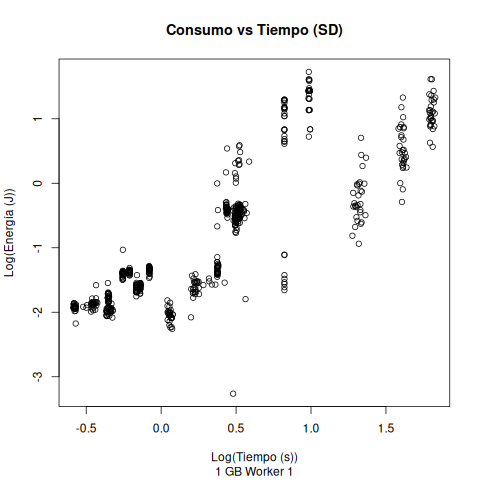
\includegraphics[width = 0.5\textwidth]{images/Dispersión-Worker1-1G-SD.png}
      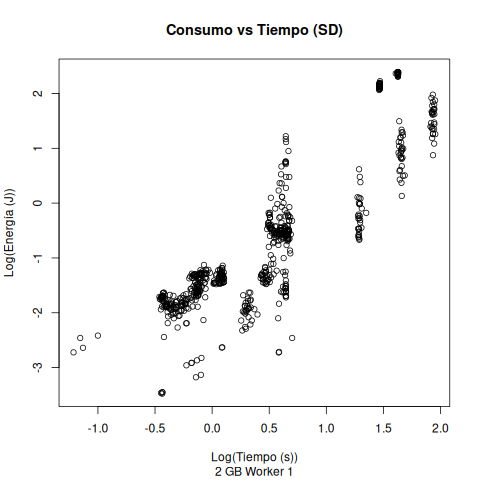
\includegraphics[width = 0.5\textwidth]{images/Dispersión-Worker1-2G-SD.png}
      \caption{Gŕaficos de dispersión de consumo del trabajador 1 para 1 GB y 2
      GB}
      \label{fig:dispersionWorker1_1SD}
    \end{figure}

    \begin{figure}[H]
      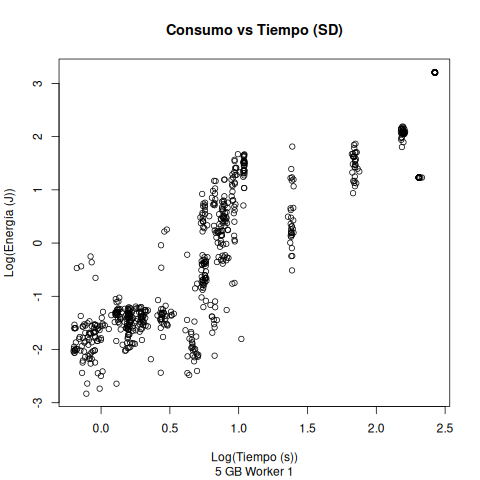
\includegraphics[width = 0.5\textwidth]{images/Dispersión-Worker1-5G-SD.png}
      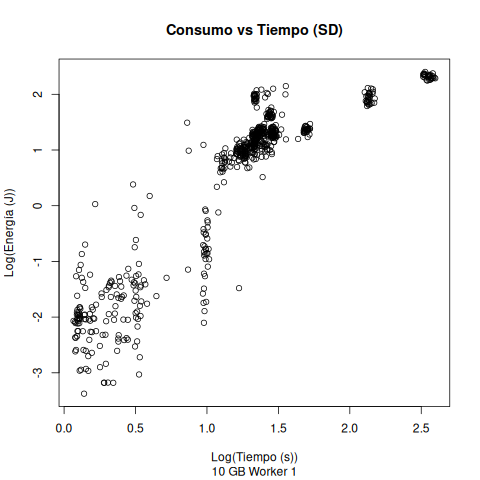
\includegraphics[width = 0.5\textwidth]{images/Dispersión-Worker1-10G-SD.png}
      \caption{Gŕaficos de dispersión de consumo del trabajador 1 para 5 GB y 10
      GB}
      \label{fig:dispersionWorker1_2SD}
    \end{figure}

    \begin{figure}[H]
      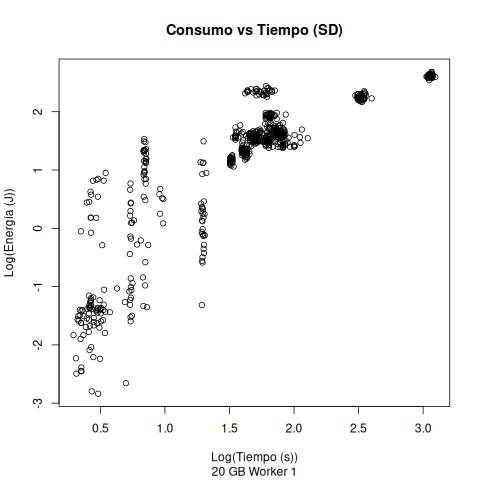
\includegraphics[width = 0.5\textwidth]{images/Dispersión-Worker1-20G-SD.png}
      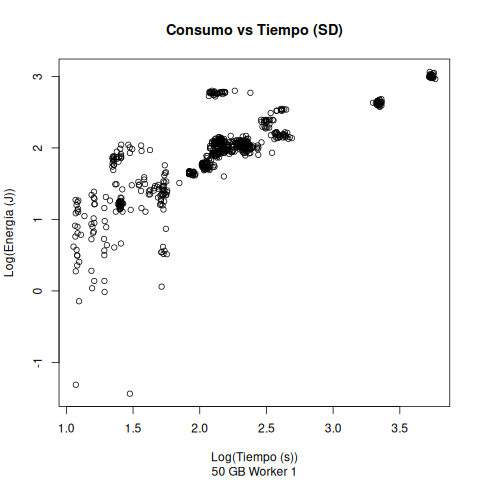
\includegraphics[width = 0.5\textwidth]{images/Dispersión-Worker1-50G-SD.png}
      \caption{Gŕaficos de dispersión de consumo del trabajador 1 para 20 GB y
      50 GB}
      \label{fig:dispersionWorker1_3SD}
    \end{figure}

    % section consumo_trabajador_1 (end)

    \section{Consumo trabajador 2} % (fold)
    \label{sec:consumo_trabajador_2}

    \begin{figure}[H]
      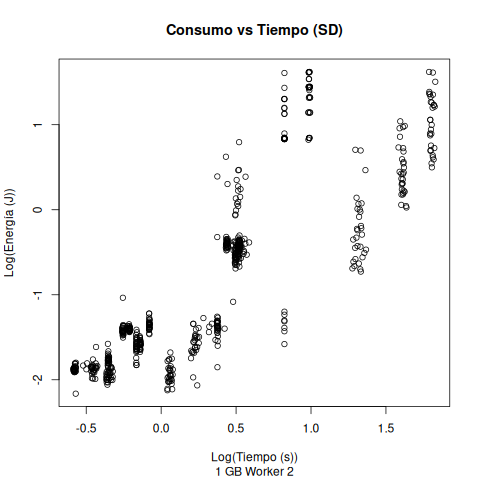
\includegraphics[width = 0.5\textwidth]{images/Dispersión-Worker2-1G-SD.png}
      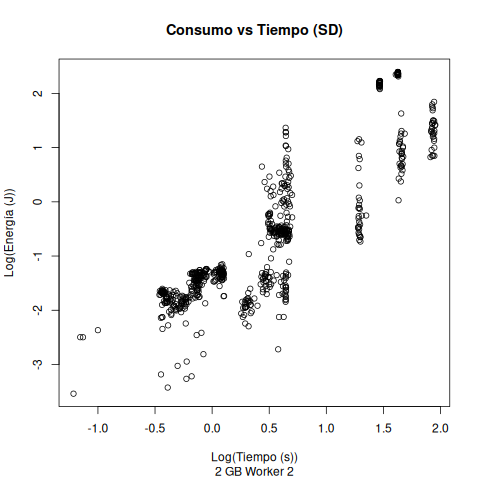
\includegraphics[width = 0.5\textwidth]{images/Dispersión-Worker2-2G-SD.png}
      \caption{Gŕaficos de dispersión de consumo del trabajador 2 para 1 GB y 2
      GB}
      \label{fig:dispersionWorker2_1SD}
    \end{figure}

    \begin{figure}[H]
      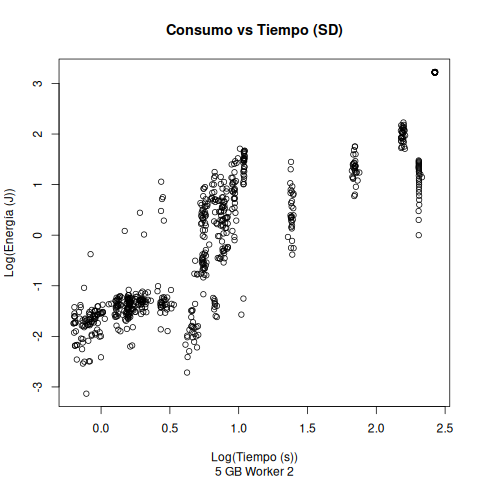
\includegraphics[width = 0.5\textwidth]{images/Dispersión-Worker2-5G-SD.png}
      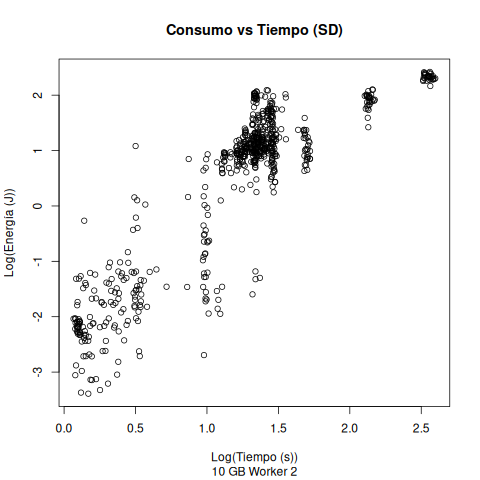
\includegraphics[width = 0.5\textwidth]{images/Dispersión-Worker2-10G-SD.png}
      \caption{Gŕaficos de dispersión de consumo del trabajador 2 para 5 GB y 10
      GB}
      \label{fig:dispersionWorker2_2SD}
    \end{figure}

    \begin{figure}[H]
      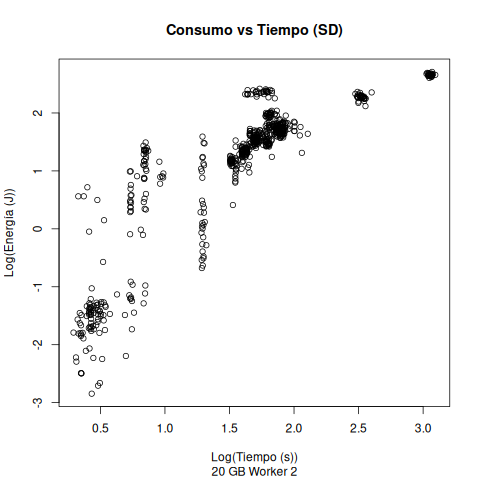
\includegraphics[width = 0.5\textwidth]{images/Dispersión-Worker2-20G-SD.png}
      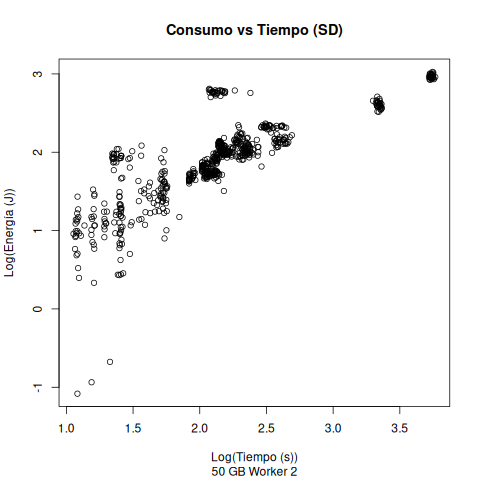
\includegraphics[width = 0.5\textwidth]{images/Dispersión-Worker2-50G-SD.png}
      \caption{Gŕaficos de dispersión de consumo del trabajador 2 para 20 GB y
      50 GB}
      \label{fig:dispersionWorker2_3SD}
    \end{figure}

    % section consumo_trabajador_2 (end)

    \section{Consumo coordinador} % (fold)
    \label{sec:consumo_coordinador}

    \begin{figure}[H]
      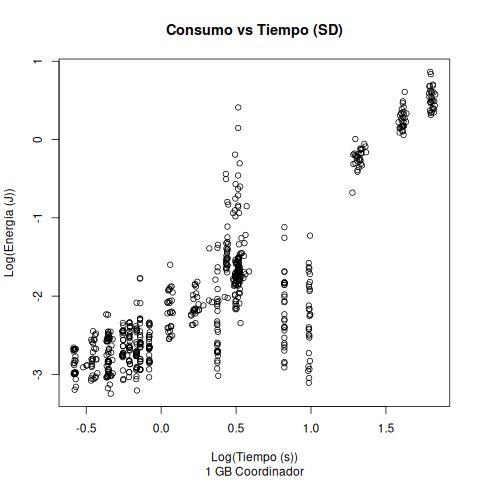
\includegraphics[width = 0.5\textwidth]{images/Dispersión-Coordinador-1G-SD.png}
      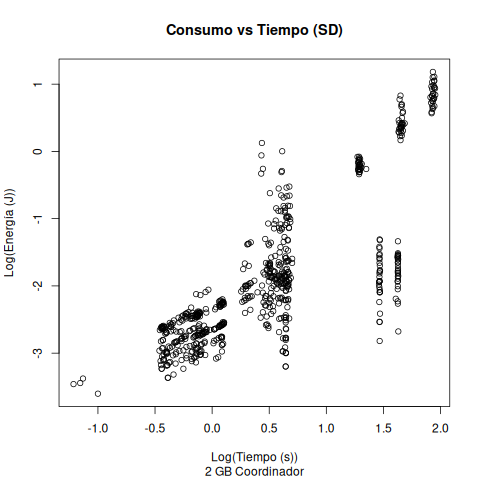
\includegraphics[width = 0.5\textwidth]{images/Dispersión-Coordinador-2G-SD.png}
      \caption{Gŕaficos de dispersión de consumo del coordinador para 1 GB y 2
      GB}
      \label{fig:dispersionCoord1SD}
    \end{figure}

    \begin{figure}[H]
      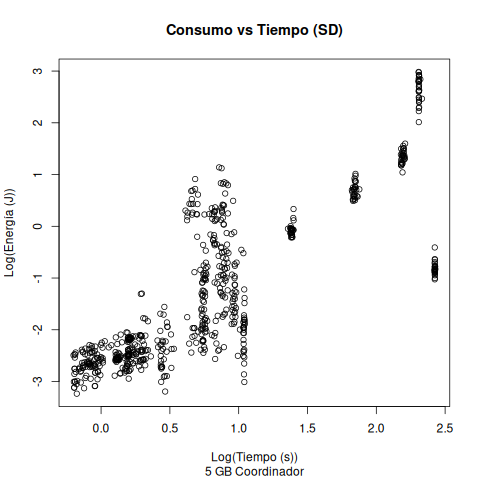
\includegraphics[width = 0.5\textwidth]{images/Dispersión-Coordinador-5G-SD.png}
      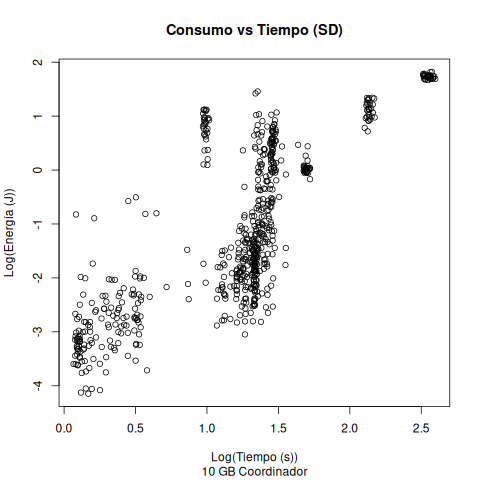
\includegraphics[width = 0.5\textwidth]{images/Dispersión-Coordinador-10G-SD.png}
      \caption{Gŕaficos de dispersión de consumo del coordinador para 5 GB y 10
      GB}
      \label{fig:dispersionCoord2SD}
    \end{figure}

    \begin{figure}[H]
      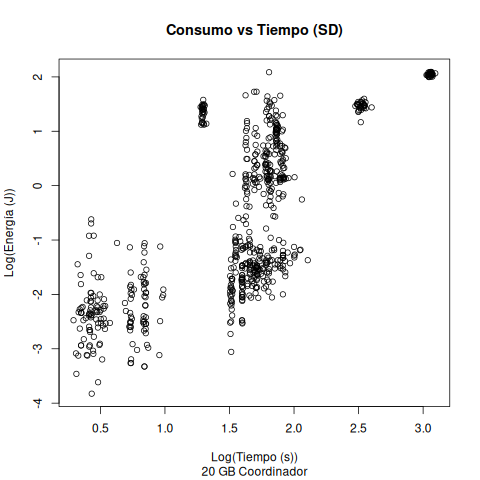
\includegraphics[width = 0.5\textwidth]{images/Dispersión-Coordinador-20G-SD.png}
      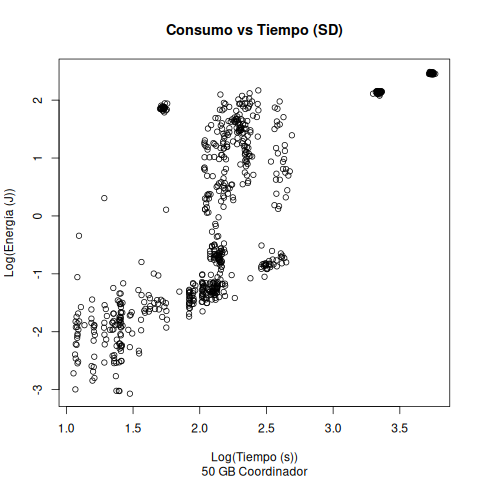
\includegraphics[width = 0.5\textwidth]{images/Dispersión-Coordinador-50G-SD.png}
      \caption{Gŕaficos de dispersión de consumo del coordinador para 20 GB y 50
      GB}
      \label{fig:dispersionCoord3SD}
    \end{figure}

    % section consumo_coordinador (end)
  % chapter graficos_de_dispersion_sin_diseno

  \chapter{Gráficos de dispersión con diseño}
  \label{apx:dispersionCD}

    \section{Consumo neto} % (fold)
    \label{sec:consumo_netoCD}
    
    \begin{figure}[H]
      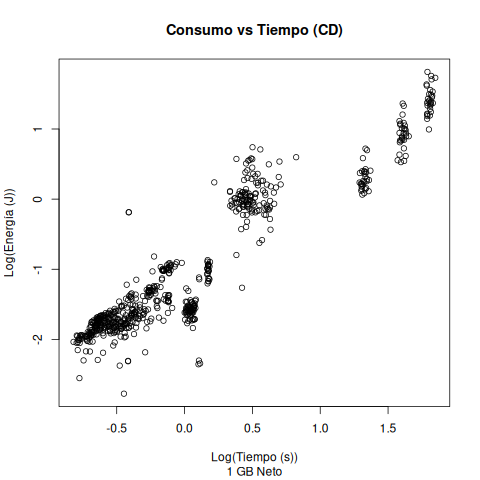
\includegraphics[width = 0.5\textwidth]{images/Dispersión-Neto-1G-CD.png}
      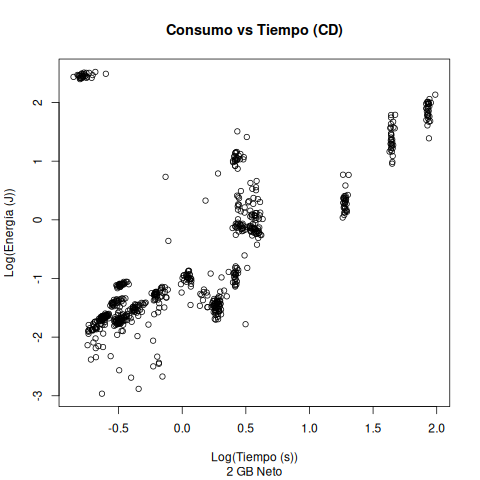
\includegraphics[width = 0.5\textwidth]{images/Dispersión-Neto-2G-CD.png}
      \caption{Gŕaficos de dispersión de consumo neto para 1 GB y 2 GB}
      \label{fig:dispersionNeto1CD}
    \end{figure}

    \begin{figure}[H]
      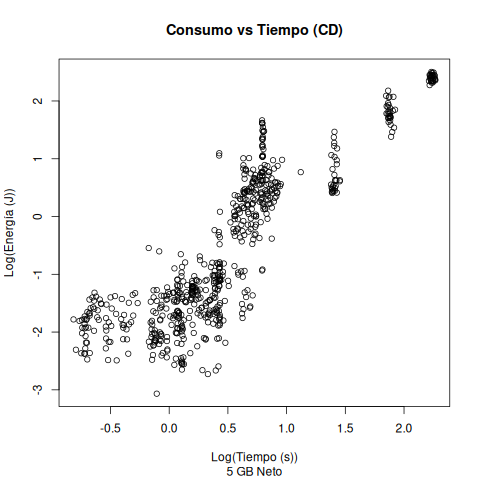
\includegraphics[width = 0.5\textwidth]{images/Dispersión-Neto-5G-CD.png}
      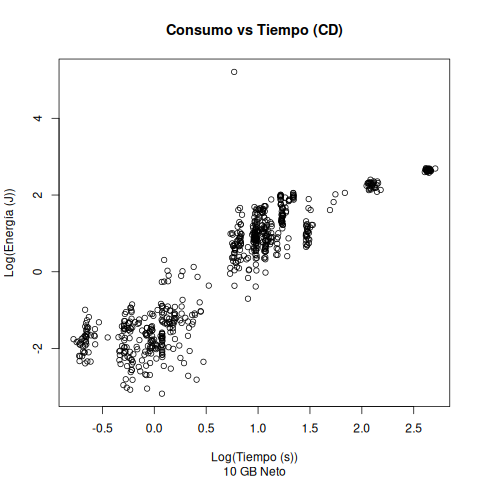
\includegraphics[width = 0.5\textwidth]{images/Dispersión-Neto-10G-CD.png}
      \caption{Gŕaficos de dispersión de consumo neto para 5 GB y 10 GB}
      \label{fig:dispersionNeto2CD}
    \end{figure}

    \begin{figure}[H]
      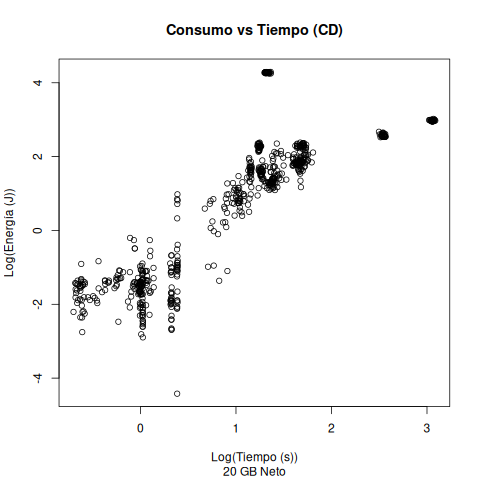
\includegraphics[width = 0.5\textwidth]{images/Dispersión-Neto-20G-CD.png}
      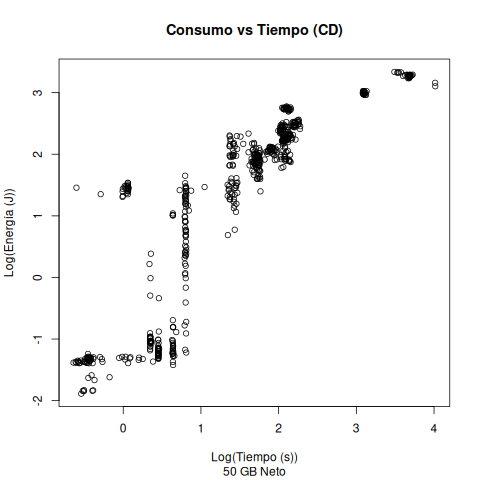
\includegraphics[width = 0.5\textwidth]{images/Dispersión-Neto-50G-CD.png}
      \caption{Gŕaficos de dispersión de consumo neto para 20 GB y 50 GB}
      \label{fig:dispersionNeto3CD}
    \end{figure}

    % section consumo_netoCD (end)

    \section{Consumo trabajador 1} % (fold)
    \label{sec:consumo_trabajador_1_CD}

    \begin{figure}[H]
      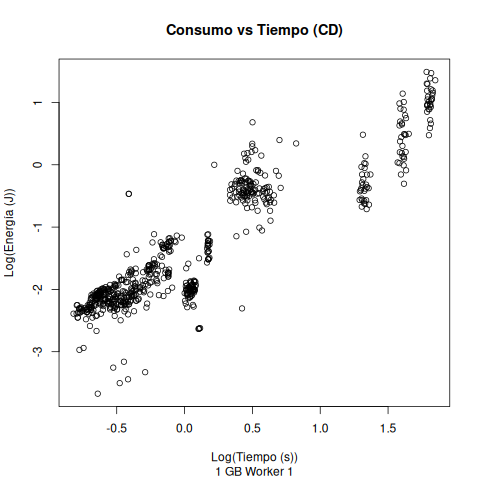
\includegraphics[width = 0.5\textwidth]{images/Dispersión-Worker1-1G-CD.png}
      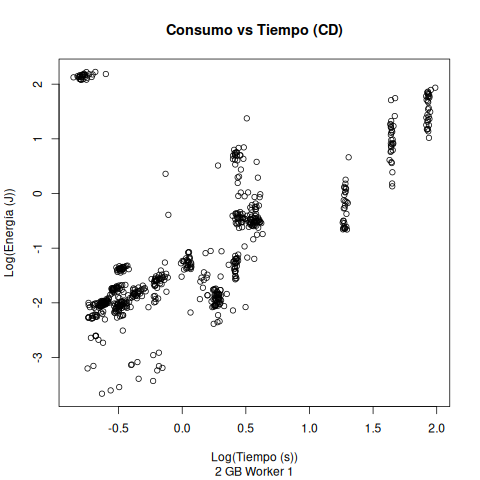
\includegraphics[width = 0.5\textwidth]{images/Dispersión-Worker1-2G-CD.png}
      \caption{Gŕaficos de dispersión de consumo del trabajador 1 para 1 GB y 2
      GB}
      \label{fig:dispersionWorker1_1CD}
    \end{figure}

    \begin{figure}[H]
      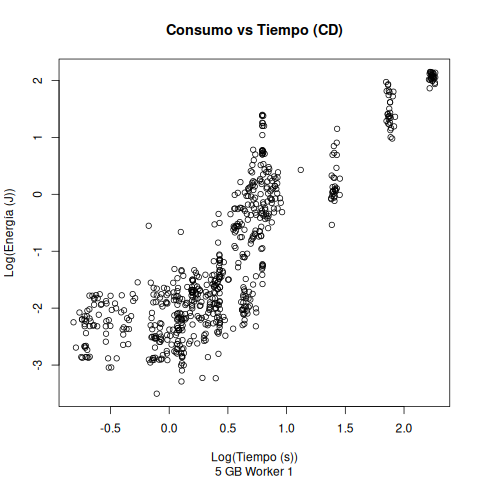
\includegraphics[width = 0.5\textwidth]{images/Dispersión-Worker1-5G-CD.png}
      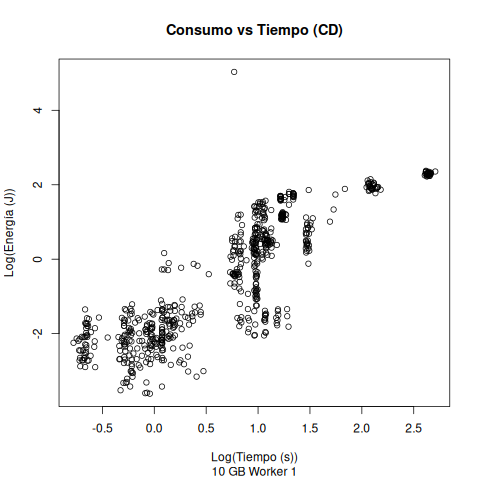
\includegraphics[width = 0.5\textwidth]{images/Dispersión-Worker1-10G-CD.png}
      \caption{Gŕaficos de dispersión de consumo del trabajador 1 para 5 GB y 10
      GB}
      \label{fig:dispersionWorker1_2CD}
    \end{figure}

    \begin{figure}[H]
      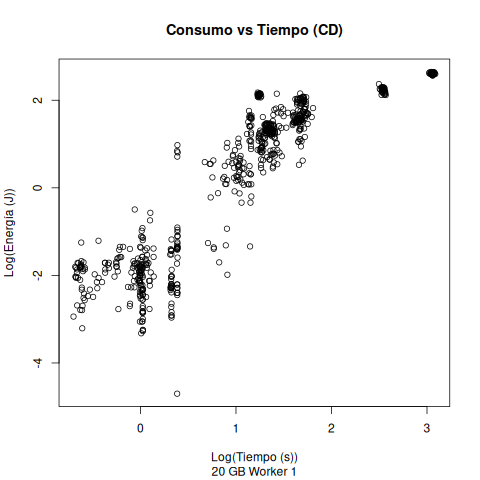
\includegraphics[width = 0.5\textwidth]{images/Dispersión-Worker1-20G-CD.png}
      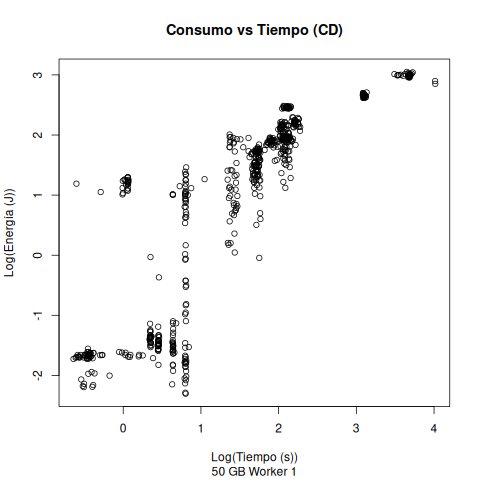
\includegraphics[width = 0.5\textwidth]{images/Dispersión-Worker1-50G-CD.png}
      \caption{Gŕaficos de dispersión de consumo del trabajador 1 para 20 GB y
      50 GB}
      \label{fig:dispersionWorker1_3CD}
    \end{figure}

    % section consumo_trabajador_1_CD (end)

    \section{Consumo trabajador 2} % (fold)
    \label{sec:consumo_trabajador_2_CD}

    \begin{figure}[H]
      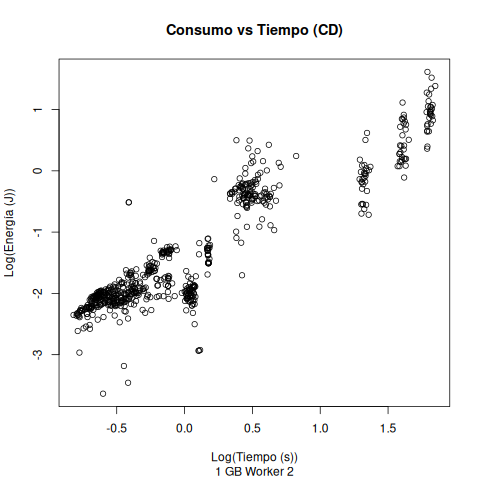
\includegraphics[width = 0.5\textwidth]{images/Dispersión-Worker2-1G-CD.png}
      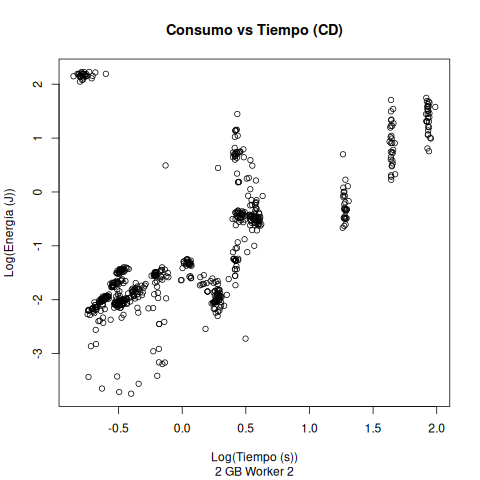
\includegraphics[width = 0.5\textwidth]{images/Dispersión-Worker2-2G-CD.png}
      \caption{Gŕaficos de dispersión de consumo del trabajador 2 para 1 GB y 2
      GB}
      \label{fig:dispersionWorker2_1CD}
    \end{figure}

    \begin{figure}[H]
      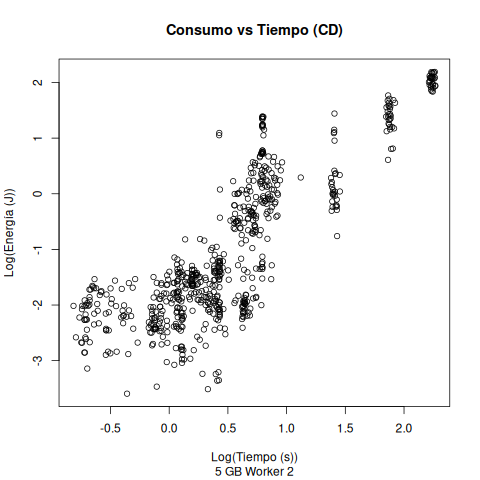
\includegraphics[width = 0.5\textwidth]{images/Dispersión-Worker2-5G-CD.png}
      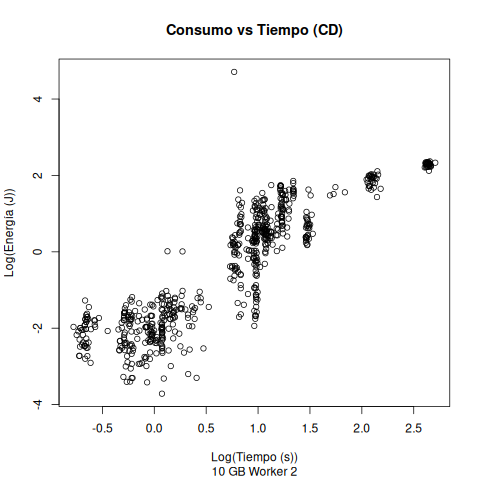
\includegraphics[width = 0.5\textwidth]{images/Dispersión-Worker2-10G-CD.png}
      \caption{Gŕaficos de dispersión de consumo del trabajador 2 para 5 GB y 10
      GB}
      \label{fig:dispersionWorker2_2CD}
    \end{figure}

    \begin{figure}[H]
      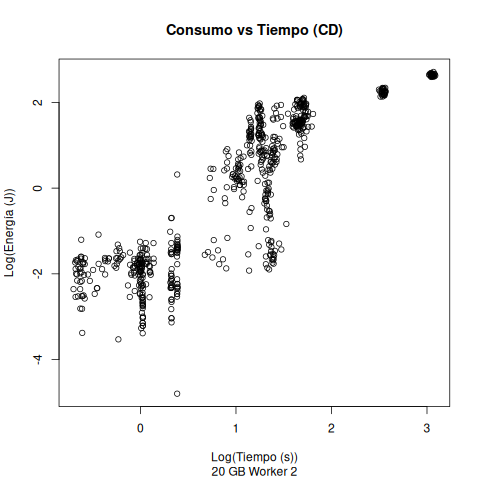
\includegraphics[width = 0.5\textwidth]{images/Dispersión-Worker2-20G-CD.png}
      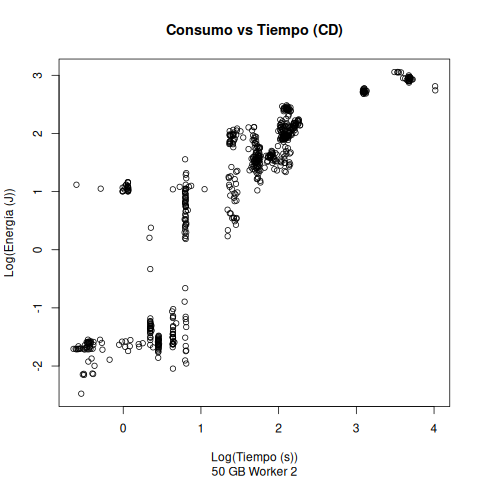
\includegraphics[width = 0.5\textwidth]{images/Dispersión-Worker2-50G-CD.png}
      \caption{Gŕaficos de dispersión de consumo del trabajador 2 para 20 GB y 50
      GB}
      \label{fig:dispersionWorker2_3CD}
    \end{figure}

    % section consumo_trabajador_2_CD (end)

    \section{Consumo coordinador} % (fold)
    \label{sec:consumo_coordinadorCD}

    \begin{figure}[H]
      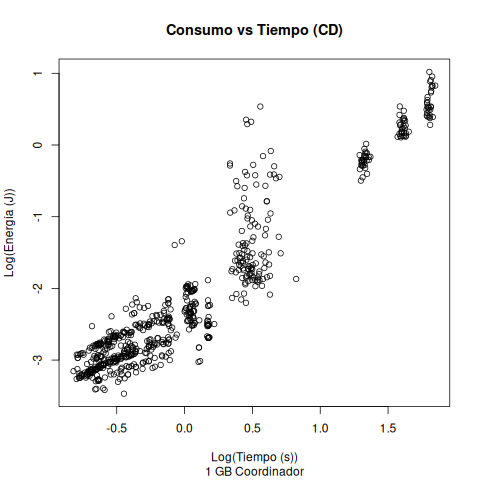
\includegraphics[width = 0.5\textwidth]{images/Dispersión-Coordinador-1G-CD.png}
      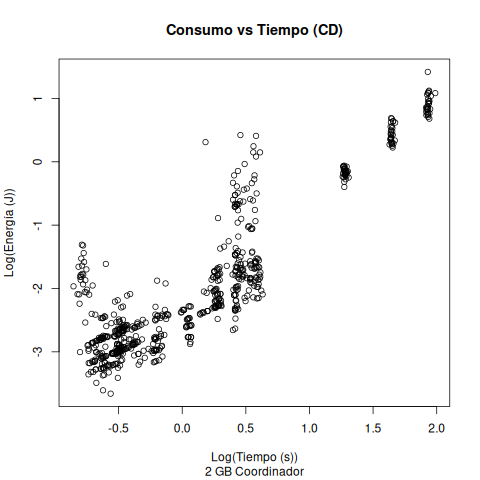
\includegraphics[width = 0.5\textwidth]{images/Dispersión-Coordinador-2G-CD.png}
      \caption{Gŕaficos de dispersión de consumo del coordinador para 1 GB y 2
      GB}
      \label{fig:dispersionCoord1CD}
    \end{figure}

    \begin{figure}[H]
      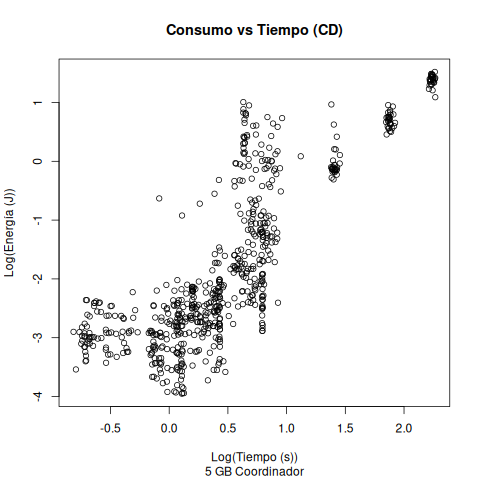
\includegraphics[width = 0.5\textwidth]{images/Dispersión-Coordinador-5G-CD.png}
      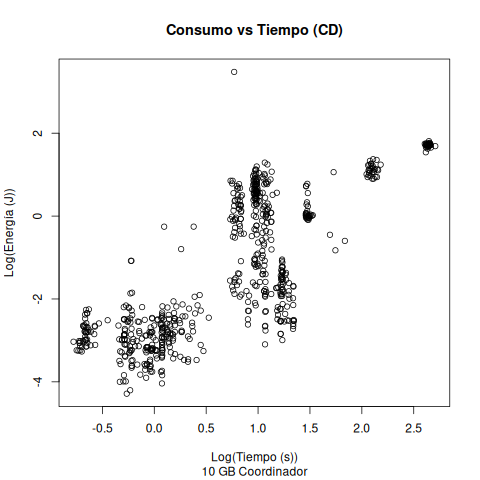
\includegraphics[width = 0.5\textwidth]{images/Dispersión-Coordinador-10G-CD.png}
      \caption{Gŕaficos de dispersión de consumo del coordinador para 5 GB y 10
      GB}
      \label{fig:dispersionCoord2CD}
    \end{figure}

    \begin{figure}[H]
      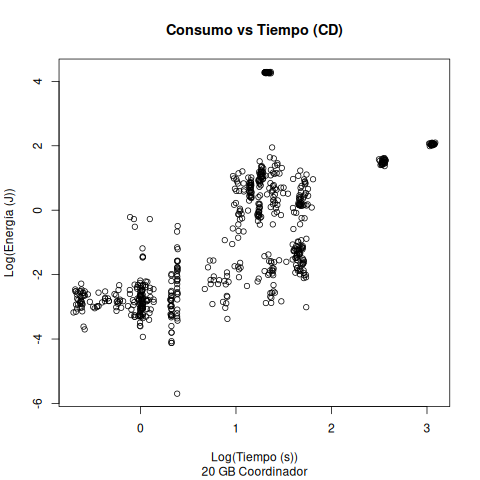
\includegraphics[width = 0.5\textwidth]{images/Dispersión-Coordinador-20G-CD.png}
      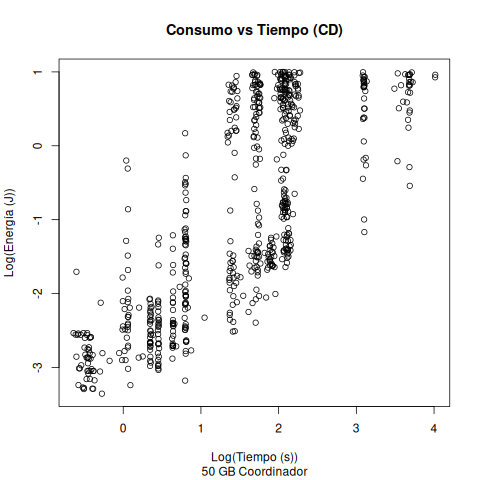
\includegraphics[width = 0.5\textwidth]{images/Dispersión-Coordinador-50G-CD.png}
      \caption{Gŕaficos de dispersión de consumo del coordinador para 20 GB y 50
      GB}
      \label{fig:dispersionCoord3CD}
    \end{figure}
    % section consumo_coordinadorCD (end)
  % chapter graficos_de_dispersion_con_diseno
\end{document}
